\RequirePackage[thinlines]{easybmat} %-- muss aufgrund eines Bugs vor etex und tikz geladen werden
\documentclass[a4paper, twoside, headsepline, index=totoc,toc=listof, fontsize=10pt, cleardoublepage=empty, headinclude, DIV=13, BCOR=13mm, titlepage,]{scrartcl}
\usepackage{scrtime} % KOMA, Uhrzeit ermoeglicht
\usepackage{scrpage2} % wie fancyhdr, nur optimiert auf KOMA-Skript, leicht andere Syntax
\usepackage{etoolbox}
\usepackage{letltxmacro}

% Compiler abhaengige IFs
\usepackage{ifxetex,ifluatex}
\newif\ifxetexorluatex
\ifxetex
  \xetexorluatextrue
\else
  \ifluatex
    \xetexorluatextrue
  \else
    \xetexorluatexfalse
  \fi
\fi

%--Farbdefinitionen
%-- muss vor tikz geladen werden
\usepackage[usenames, table, x11names]{xcolor}
\definecolor{dark_gray}{gray}{0.45}
\definecolor{light_gray}{gray}{0.6}

%--Zum Zeichnen
%-- muss vor polyglossia bzw. babel geladen werden
\usepackage{tikz}
\usepackage{tikz-cd}
\usetikzlibrary{external}
\tikzset{>=latex}
\usetikzlibrary{shapes,arrows,intersections}
\usetikzlibrary{calc,3d}
\usetikzlibrary{decorations.pathreplacing,decorations.markings}
\usetikzlibrary{angles}

%-- Konfiguration von tikzexternalize
\tikzexternalize[prefix=tikz/, up to date check=diff]

\ifxetexorluatex
\tikzset{external/system call={xelatex \tikzexternalcheckshellescape %-- verwende LuaLaTeX, wegen dynamischer Speicherallokation
    -halt-on-error -interaction=batchmode -jobname "\image" "\texsource"}}
\else
\tikzset{external/system call={pdflatex \tikzexternalcheckshellescape 
    -halt-on-error -interaction=batchmode -jobname "\image" "\texsource"}}
\fi

%-- tikzexternalize fuer tikzcd deaktivieren, da inkompatibel
\AtBeginEnvironment{tikzcd}{\tikzexternaldisable}
\AtEndEnvironment{tikzcd}{\tikzexternalenable}

%-- um Inkompatibilitaeten von quotes und polyglossia bzw. babel zu vermeiden
\tikzset{
  every picture/.append style={
    execute at begin picture={\shorthandoff{"}},
    execute at end picture={\shorthandon{"}}
  }
}
\usetikzlibrary{quotes}
\usepackage{pgfplots}
\usepgfplotslibrary{colormaps}
\pgfplotsset{compat=1.10}



%-- Mathe
\usepackage{mathtools} % beinhaltet amsmath
\mathtoolsset{showonlyrefs, centercolon}
\newtagform{brackets}[\textbf]{[}{]}
\usetagform{brackets}
\usepackage{wasysym}
\usepackage{amssymb} %zusätzliche Symbole
\usepackage{latexsym} %zusätzliche Symbole
\usepackage{stmaryrd} %für Blitz
\usepackage{nicefrac} %schräge Brüche
\usepackage{cancel} %Befehle zum Durchstreichen
\usepackage{mathdots}
% \usepackage{bm}
\DeclareSymbolFont{bbold}{U}{bbold}{m}{n}
\DeclareSymbolFontAlphabet{\mathbbold}{bbold}
\newcommand{\mathds}[1]{\mathbb{#1}} %Um Kompatibilitaet mit frueheren Benutzung von dsfont herzustellen
\newcommand{\ind}{\mathbbold{1}} % charakteristische-Funktion-Eins
\def\mathul#1#2{\color{#1}\underline{{\color{black}#2}}\color{black}} %farbiges Untersteichen im Mathe-Modus

%-- Alles was mit Schrift und XeteX zu tun hat
\ifxetexorluatex
    % XeLaTeX or LuaTeX
	\ifxetex
		\usepackage{mathspec} %beinhaltet fontspec 
	\else
		\usepackage[no-math]{fontspec}
	\fi
    \usepackage{polyglossia} %babel-ersatz
    \setmainlanguage[spelling=new,babelshorthands=false]{german}
	\newcommand\glqq{"}
	\newcommand\grqq{"}
	\defaultfontfeatures{Mapping=tex-text, WordSpace={1.4}} %
    \setmainfont[Ligatures=Common, BoldFont={* Bold}, ItalicFont={* Light Italic},SmallCapsFont={Linux Libertine O}, SmallCapsFeatures={Letters=SmallCaps}]{Source Sans Pro}
	\setsansfont[Scale=MatchLowercase,Ligatures=Common, BoldFont={* Medium}]{Ubuntu}
	\ifxetex
		\setallmonofonts[Scale=MatchLowercase, ItalicFont={*}]{Consolas} 
	\else
		\setmonofont[Scale=MatchLowercase, ItalicFont={*}]{Consolas}
	\fi
	\usepackage{xltxtra}
	\usepackage{fontawesome}
	\usepackage{microtype}
\else
    % default: pdfLaTeX
    \usepackage[ngerman]{babel}
    \usepackage[T1]{fontenc}
    \usepackage[utf8]{inputenc}
	\usepackage{textcomp} %verhindert ein paar Fehler bei den Fonts
    \usepackage[babel=true, tracking=true]{microtype}
	\usepackage{lmodern}
	\renewcommand{\familydefault}{\sfdefault} 
\fi


%--Mixed
\usepackage[neverdecrease]{paralist}
\usepackage[german=quotes]{csquotes}
\usepackage{makeidx}
\usepackage{booktabs}
\usepackage{wrapfig}
\usepackage{float}
\usepackage[margin=10pt, font=small, labelfont={sf, bf}, format=plain, indention=1em]{caption}
\captionsetup[wrapfigure]{name=Abb. }
\usepackage{stackrel}
\usepackage{ifthen}
\usepackage{multicol}
\usepackage{qrcode}
\flushbottom

%--Hyphenation
\hyphenation{di-men-si-o-na-le}


%--Unterstreichung
\usepackage[normalem]{ulem}
\setlength{\ULdepth}{1.8pt}

%--Indexverarbeitung
\newcommand{\bet}[1]{\textbf{#1}}
\newcommand{\Index}[1]{\textbf{#1}\index{#1}}
\makeindex
\setindexpreamble{{\noindent \itshape Die \emph{Seitenzahlen} sind mit Hyperlinks zu den entsprechenden Seiten versehen, also anklickbar} \ifxetexorluatex \faHandUp\fi \par \bigskip}
\renewcommand{\indexpagestyle}{scrheadings}


%--Marginnote & todonotes
\usepackage{marginnote}
\renewcommand*{\marginfont}{\color{dark_gray} \itshape \footnotesize }
\usepackage[textsize=small]{todonotes}

%--Todonotes mit tikz/externalize kompatibel machen
\LetLtxMacro{\oldtodo}{\todo}
\renewcommand{\todo}[2][]{\tikzexternaldisable\oldtodo[#1]{#2}\tikzexternalenable}
\LetLtxMacro{\oldmissingfigure}{\missingfigure}
\renewcommand{\missingfigure}[2][]{\tikzexternaldisable\oldmissingfigure[{#1}]{#2}\tikzexternalenable}

%--Konfiguration von Hyperref pdfstartview=FitH, 
\usepackage[hidelinks, pdfpagelabels,  bookmarksopen=true, bookmarksnumbered=true, linkcolor=black, urlcolor=SkyBlue2, plainpages=false,pagebackref, citecolor=black, hypertexnames=true, pdfauthor={Jannes Bantje}, pdfborderstyle={/S/U}, linkbordercolor=SkyBlue2, colorlinks=false]{hyperref}

% \let\orighref\href
\ifxetexorluatex
\newcommand{\hrefsym}[2]{\href{#1}{\texttt{#2\,\faExternalLink}}}
\newcommand{\hrefsymmail}[2]{\href{#1}{\texttt{\faEnvelope\,#2}}}
\renewcommand{\url}[1]{\hrefsym{#1}{\nolinkurl{#1}}}
\fi
\providecommand{\hrefsym}{\href}
% \usepackage{cleveref}
% \crefformat{footnote}{#2\footnotemark[#1]#3}

%--Römische Zahlen
\newcommand{\RM}[1]{\MakeUppercase{\romannumeral #1{}}}

%--Punkte (nach hyperref)
\usepackage{ellipsis}

%%--Abkürzungen etc.
\newcommand{\light}{\text{\Large $\lightning$}}

%-- Definitionen von weiteren Mathe-Befehlen
\DeclareMathOperator{\re}{Re} %Realteil
\DeclareMathOperator{\im}{Im} %Imaginaerteil
\DeclareMathOperator{\id}{id} %identische Abbildung
\DeclareMathOperator{\Sp}{Sp} %Spur
\DeclareMathOperator{\sgn}{sgn} %Signum
\DeclareMathOperator{\alt}{Alt} %Alternierende n-linearFormen
\DeclareMathOperator{\End}{End} %Endomorphismen
\DeclareMathOperator{\Vol}{Vol} %Volumen
\DeclareMathOperator{\dom}{dom} %Domain
\DeclareMathOperator{\Hom}{Hom} %Homomorphismen
\DeclareMathOperator{\bild}{Bild} %Bild
\DeclareMathOperator{\Kern}{Kern }
\DeclareMathOperator{\rg}{rg} %Rang
\DeclareMathOperator{\Rg}{Rg} %Rang
\DeclareMathOperator{\diam}{diam} %Durchmesser
\DeclareMathOperator{\dist}{dist} %Distanz
\DeclareMathOperator{\grad}{grad} %Gradient
\DeclareMathOperator{\dive}{div} %Gradient
\DeclareMathOperator{\rot}{rot} %Rotation
\DeclareMathOperator{\hess}{Hess} %Hesse-Matrix
\DeclareMathOperator{\koker}{Koker} %Kokern
\DeclareMathOperator{\aut}{Aut} %Automorphismen
\DeclareMathOperator{\ord}{ord} %Ordnung
\DeclareMathOperator{\ggT}{ggT} %ggT
\DeclareMathOperator{\kgV}{kgV} %kgV
\DeclareMathOperator{\Gr}{Gr} %Gerade
\DeclareMathOperator{\Kr}{Kr} %Kreis
\DeclareMathOperator{\Char}{char} %Charakteristik
\DeclareMathOperator{\Aut}{Aut} %Automorphismen
% \DeclareMathOperator{\D}{D} %formale Ableitung
\newcommand{\D}{\ensuremath{\mathrm{D}\mkern-1.5mu}}
\newcommand{\mathd}{\ensuremath{\mathrm{d}\mkern-1.0mu}}
\newcommand{\Tmap}{\ensuremath{\mathrm{T}\mkern-1.0mu}}
\newcommand{\opL}{\ensuremath{\mathrm{L}\mkern-0.6mu}}
\DeclareMathOperator{\cov}{cov} %Kovarianz
\DeclareMathOperator{\Gal}{Gal} %Galois
\DeclareMathOperator{\supp}{supp} %Träger
\DeclareMathOperator{\Sym}{Sym} %Symmetrische Gruppe
\DeclareMathOperator{\Zyl}{Zyl} %Zylinder
\DeclareMathOperator{\Mod}{Mod} %Moduln
\DeclareMathOperator{\EPK}{EPK} %Einpunktkompaktifizierung
\DeclareMathOperator{\conj}{conj} %Konjugation
\DeclareMathOperator{\ann}{ann} %Annulator
\DeclareMathOperator{\tor}{tor} %Torsionsmodul
\DeclareMathOperator{\Int}{Int} %Interior/Inneres
\DeclareMathOperator{\Br}{Br} %Brauerergruppe
\DeclareMathOperator{\GL}{GL} %allgemeine lineare Gruppe
\DeclareMathOperator{\SL}{SL} %spezielle lineare Gruppe
\DeclareMathOperator{\SU}{SU} %spezielle unitäre Gruppe
\DeclareMathOperator{\Tr}{Tr} %Spur/Trace
\DeclareMathOperator{\conv}{conv} %Konvexe Teilmenge
% \DeclareMathOperator{\tr}{tr}
\newcommand{\tr}{\mathrm{tr}}
\newcommand{\w}{\mathrm{w}}
\newcommand{\weakT}[1]{\ensuremath{\mathcal{T}_{#1}^{\mkern+1.0mu\text{\raisebox{0.4ex}{$\mathrm{w}$}}}}}
\newcommand{\weakTstar}[1]{\ensuremath{\mathcal{T}_{#1}^{\mkern+1.0mu\text{\raisebox{0.4ex}{$\mathrm{w}$}}^*}}}
\newcommand{\rand}[1]{\ensuremath{\partial^{\scriptscriptstyle #1}}}


% -- Kategorien
\DeclareMathOperator{\Ob}{Ob} %Objekte
\DeclareMathOperator{\Mor}{Mor} %Morphismen

% \DeclareMathOperator{\TOP}{TOP} %Topologische Räume
\newcommand{\TOP}{\textsc{Top}}
% \DeclareMathOperator{\HTOP}{HTOP} %Topologische Räume + Homotopieäquivalenz
\newcommand{\HTOP}{\textsc{HTop}}
% \DeclareMathOperator{\VR}{VR} %Vektorräume
\newcommand{\VR}{\textsc{VR}}
% \DeclareMathOperator{\MOD}{MOD} %Moduln
\newcommand{\MOD}{\textsc{Mod}}
% \DeclareMathOperator{\MENGEN}{MENGEN} %Mengen
\newcommand{\MENGEN}{\textsc{Mengen}}
% \DeclareMathOperator{\MAN}{MAN} %Mannigfaltigkeiten
\newcommand{\MAN}{\textsc{Man}}
% \DeclareMathOperator{\GRUPPEN}{GRUPPEN} %Gruppen
\newcommand{\GRUPPEN}{\textsc{Gruppen}}
% \DeclareMathOperator{\ABELGRUPPEN}{ABEL.GRUPPEN} %abelsche Gruppen
\newcommand{\ABELGRUPPEN}{\textsc{Abel.Gruppen}}
% \DeclareMathOperator{\KAT}{KAT} %Kategorien
\newcommand{\KAT}{\textsc{Kat}}
% \DeclareMathOperator{\FUN}{FUN} %Funktoren
\newcommand{\FUN}{\textsc{Fun}}


\newcommand{\op}{\mathrm{op}}

\newcommand{\Ker}{\ensuremath{\Kern \,}}
\newcommand{\zirkel}{\rotatebox[origin = c]{-90}{$\varangle$}}
\newcommand{\wirkung}{\!\curvearrowright\!}

\newcommand{\oE}{\OE}

%--Beweisende
\newcommand{\bewende}{\ifmmode \tag*{$\square$} \else \hfill $\square$ \fi}

%--Volumen
\newcommand{\vol}[1]{\ensuremath{\Vol_{#1}}}

%--Skalarprodukt
\DeclarePairedDelimiterX\sprod[2]{\langle}{\rangle}{#1\,\delimsize\vert\,#2}

%--Betrag, Gaußklammer
\DeclarePairedDelimiter{\abs}{\lvert}{\rvert}
\DeclarePairedDelimiter{\ceil}{\lceil}{\rceil}

%--Norm
\DeclarePairedDelimiter\doppelstrich{\Vert}{\Vert}
\newcommand{\norm}[2][\relax]{
\ifx#1\relax \ensuremath{\doppelstrich*{#2}}
\else \ensuremath{\doppelstrich*{#2}_{#1}}
\fi}


%--Umklammern
\DeclarePairedDelimiter\enbrace{(}{)}
\DeclarePairedDelimiter\benbrace{[}{]}
\DeclarePairedDelimiter\lenbrace{<}{>}

%--Mengen
\DeclarePairedDelimiterX\mengenA[1]{\lbrace}{\rbrace}{#1}
\DeclarePairedDelimiterX\mengenB[2]{\lbrace}{\rbrace}{#1\, \delimsize\vert \, #2}

\makeatletter
\newcommand{\set}[2][\relax]{
\ifx#1\relax \ensuremath{
\mengenA*{#2}}
\else \ensuremath{%
  \mengenB*{#1}{#2}}
\fi}
\makeatother


%--offen und abgeschlossen
\newcommand{\off}{\! \stackrel[\text{offen}]{}{\subset} \!}
\newcommand{\abg}{\! \stackrel[\text{abg.}]{}{\subset} \!}

%--Differential
\newcommand{\diff}[2]{\ensuremath{\frac{{\partial #1}}{{\partial #2}} }}
\newcommand{\diffd}[2]{\ensuremath{\frac{\mathd #1}{\mathd #2} }}

%--Diagonale Linien für Matrizen
\newcommand\tikzmark[1]{%
  \tikzexternaldisable\tikz[overlay,remember picture,baseline] \node [anchor=base] (#1) {};\tikzexternalenable}

\newcommand\MyLine[3][]{%
  \tikzexternaldisable\begin{tikzpicture}[overlay,remember picture]
    \draw[#1] (#2.south) -- (#3.north);
  \end{tikzpicture}\tikzexternalenable}
  
%--Jordankasten
\newcommand{\Jord}{ \tikzexternaldisable \begin{BMAT}{|ccc|}{|ccc|} %
				0 & & \\ %
				1\tikzmark{z} &  \diagdown & \\ %
				& \tikzmark{u}1 \MyLine[thick]{z}{u} &  0 %
			\end{BMAT} \tikzexternalenable}
			
%--Jordankasten mit Lambda
\newcommand{\JordLa}[1][\empty]{%
	\tikzexternaldisable\ifthenelse{\equal{#1}{\empty}}
		{\begin{BMAT}{|ccc|}{|ccc|} %
				\lambda & & \\ %
				1\tikzmark{z} &  \diagdown & \\ %
				& \tikzmark{u}1 \MyLine[thick]{z}{u} &  \lambda  %
			\end{BMAT}}
		{\begin{BMAT}{|ccc|}{|ccc|} %
				\lambda_{#1}  & & \\ %
				1\tikzmark{z} &  \diagdown & \\ %
				& \tikzmark{u}1 \MyLine[thick]{z}{u} &  \lambda_{#1}  %
			\end{BMAT}}\tikzexternalenable}

%--Inhaltsverzeichnis
\usepackage[tocindentauto]{tocstyle}
\usetocstyle{KOMAlike}			

\newcommand{\fach}{Analysis \RM{2}.}
\newcommand{\semester}{SoSe 2013}
\newcommand{\homepage}{http://wwwmath.uni-muenster.de/u/wilhelm.winter/wwinter/analysis_II.html}
\newcommand{\prof}{Prof.\,Dr.\,Wilhelm Winter}
\providecommand{\verfasser}{Jannes Bantje}

%--Konfiguration von scrheadings
\setheadsepline{1pt}[\color{light_gray}]
\pagestyle{scrheadings}
%\fancyhf[H, F]{}
\clearscrheadfoot

\providecommand{\shortFach}{\fach}
\lehead{ 
\includegraphics[height=0.5 cm,keepaspectratio]{../!config/Bilder/Logo_WWU_Muenster_light_gray.pdf}}
\rehead{\rule{0cm}{0.5cm}\footnotesize \sffamily \color{light_gray} \verfasser -- Mitschrift \shortFach}
\lohead{\rule{0cm}{0.5cm} \footnotesize \sffamily \color{light_gray} Stand: \today \; \thistime[:]}
\rohead{
\includegraphics[height=0.5 cm,keepaspectratio]{../!config/Bilder/fb10logo_gray.pdf}}


\ofoot[{ \color{dark_gray} \LARGE \sffamily \thepage}]{{ \color{dark_gray} \LARGE \sffamily \thepage}} %hier wir auch der plain Stil bearbeitet!
\automark{section}
\ifoot{ \color{dark_gray} \small \leftmark}

%--Metadaten
\author{\verfasser}
\titlehead{
\includegraphics[height=1.5cm, keepaspectratio]{../!config/Bilder/Logo_WWU_Muenster.pdf}%
\hfill 
\includegraphics[height=1.3cm, keepaspectratio]{../!config/Bilder/fb10logo.pdf}}
\title{Skript \fach}
\subtitle{Mitschrift der Vorlesung  \enquote{\fach} von \prof}

\publishers{
Aktuelle Version verfügbar bei: \bigskip\\
\normalsize
\begin{minipage}[t]{0.45\textwidth}
	\centering{
	\qrcode[height=3.5cm, version=4]{https://github.com/JaMeZ-B/latex-wwu}
	\medskip\\
	
\includegraphics[height=0.4cm, keepaspectratio]{../!config/Bilder/github_octo.pdf} 
	
\includegraphics[height=0.4cm, keepaspectratio]{../!config/Bilder/GitHub_Logo.pdf} (inklusive Sourcecode)\\
	{\small\url{https://github.com/JaMeZ-B/latex-wwu}}}
\end{minipage}
\hfill
\begin{minipage}[t]{0.45\textwidth}
	\centering{
	\qrcode[height=3.5cm, version=4]{btsync://B6WH2DISQ5QVYIRYIEZSF4ZR2IDVKPN3I?n=latex_share}
	\medskip\\
	
\includegraphics[height=0.4cm, keepaspectratio]{../!config/Bilder/bt_sync_logo.pdf} 
	{\large \textbf{Bittorrent} Sync} \\
	\texttt{B6WH2DISQ5QVYIRYIEZSF4ZR2IDVKPN3I}
	}
\end{minipage}
}



\begin{document}
\pagenumbering{Roman}
\maketitle
\begin{abstract}
\section*{Vorwort --- Mitarbeit am Skript}
Dieses Dokument ist eine Mitschrift aus der Vorlesung \enquote{\fach, \semester}, gelesen von \prof. Der Inhalt entspricht weitestgehend dem Tafelanschrieb. Für die
Korrektheit des Inhalts übernehme ich keinerlei Garantie! Für Bemerkungen und Korrekturen -- und seien es nur Rechtschreibfehler -- bin ich sehr dankbar. 
Korrekturen lassen sich prinzipiell auf drei Wegen einreichen: 
\begin{itemize}
	\item Persönliches Ansprechen in der Uni, Mails an \hrefsymmail{mailto:\mail}{\mail} (gerne auch mit annotieren PDFs) 
	\item \emph{Direktes} Mitarbeiten am Skript: Den Quellcode poste ich auf GitHub (siehe oben), also stehen vielfältige Möglichkeiten der Zusammenarbeit zur Verfügung:
	Zum Beispiel durch Kommentare am Code über die Website und die Kombination Fork + Pull Request. Wer sich verdient macht oder ein Skript zu einer Vorlesung, die 
	ich nicht besuche, beisteuern will, dem gewähre ich gerne auch Schreibzugriff.
	
	Beachten sollte man dabei, dass dazu ein Account bei \url{github.com} notwendig ist, der allerdings ohne Angabe von persönlichen Daten angelegt werden kann. 
	Wer bei GitHub (bzw. dem zugrunde liegenden Open-Source-Programm \enquote{\texttt{git}}) -- verständlicherweise -- Hilfe beim Einstieg braucht, dem helfe ich gerne 
	weiter. Es gibt aber auch zahlreiche empfehlenswerte Tutorials im Internet.\footnote{zB. \url{https://try.github.io/levels/1/challenges/1}, ist auf Englisch, aber dafür 
	interaktives LearningByDoing}
	\item \emph{Indirektes} Mitarbeiten: \TeX-Dateien per Mail verschicken. 
	
	Dies ist nur dann sinnvoll, wenn man einen ganzen Abschnitt ändern möchte (zB. einen alternativen Beweis geben), da ich die Änderungen dann per Hand einbauen muss! Ich freue mich aber auch über solche Beiträge!
\end{itemize}
\section*{Vorlesungshomepage}
{\centering 
\begin{minipage}[c][][c]{\textwidth}
	\centering \qrcode[height=3cm]{\homepage} \medskip\\
	\footnotesize \url{\homepage}
\end{minipage}
\par}

\end{abstract}

\setcounter{page}{1}
\tableofcontents
\cleardoubleoddemptypage
\pagenumbering{arabic}
\setcounter{page}{1}


\section{Funktionenfolgen und Potenzreihen} % (fold)
\label{sec:funktionenfolgen_und_potenzreihen}

\subsection[Definition Konvergenz von Funktionenfolgen]{Definition} % (fold)
\label{sub:11}
Sei $M$ eine Menge und $f : M \to \mathds{C}$ , $f_n : M \to \mathds{C}, n \in \mathds{N} $ Funktionen \index{Funktionenfolgen!punktweise Konvergenz}
\begin{enumerate}[a)]
	\item $f_n \xrightarrow{n \to \infty} f$ punktweise, falls für jedes $x \in M$ $f_n(x) \xrightarrow{n \to \infty} f(x)$ gilt. D.h.
	\[
		\forall x \in M \, \forall \varepsilon > 0 \exists N \in \mathds{N} : \forall n \ge N : \abs*{f_n(x) - f(x)} < \varepsilon
	\]
	\item $f_n \xrightarrow{n \to \infty} f$ gleichmäßig, falls gilt: \index{Funktionenfolgen!gleichmäßige Konvergenz}
	\[
		\forall \varepsilon >0 \, \exists N \in \mathds{N} : \forall x \in M , n \ge N : \abs*{f_n(x) - f(x)} < \varepsilon
	\]
	\item $\norm[\infty, M]{f} := \sup \big\{ \abs*{f(x)} \mid x \in M \big\} \in [0, \infty)$
\end{enumerate}
% subsection 11 (end)

\subsection[Bemerkung zur Normen]{Bemerkung} % (fold)
\label{sub:12}
\begin{enumerate}[(i)]
	\item gleichmäßige Konvergenz $\Longrightarrow $ punktweise Konvergenz
	\item $\norm[\infty, M]{f} < \infty \iff f$ beschränkt
	\item \label{12:enum:3}$\norm[\infty, M]{.}$ ist eine Norm auf $\{ f: M \to \mathds{C} \mid f \text{ beschränkt}\}$ \hfill (Übung)
	
	$V$ Vektorraum über $\mathds{K}$. $\norm{.} : V \to \mathds{R}_+$ ist eine \Index{Norm}  falls gilt: \index{Norm!Supremumsnorm}
	\begin{enumerate}[(i)]
		\item $\norm{v}=0 \iff v = 0$
		\item $\norm{\lambda \cdot v} = \abs*{\lambda } \cdot \norm{v}$
		\item $\norm{v+w} \le \norm{v} + \norm{w}$
	\end{enumerate}
	\item $f_n \xrightarrow{n \to \infty} f$ gleichmäßig $\iff \norm[\infty,M]{f_n -f} \xrightarrow{n \to \infty} 0$  \hfill (Übung)
\end{enumerate}
% subsection 12 (end)

\subsection[Beispiele von konvergierenden Funktionenfolgen]{Beispiele} % (fold)
\label{sub:13}
\begin{enumerate}[(i)]
	\item 
	$f_n$ aus Abb. \ref{fig:konvFkt} konvergiert punktweise gegen 0, aber $f_n$ konvergiert nicht gleichmäßig gegen 0, denn 
	\[
		\norm[\infty, M]{f_n -0} = 1 \enspace \forall n \in \mathds{N}^* 
	\]
	\begin{figure}[ht]
		\centering{
		\begin{tikzpicture}
			%\draw[help lines] (0,0) grid (6,3);
			\draw[<->, thick] (0,3.2) -- (0,0) -- (6.2 ,0);
			\draw[red, ultra thick] (0,0) -- (1.5 , 3) -- (3,0) -- (6,0);
			\node [left] at (0,3) {1};
			\node [below] at (1.5 , 0) {$\frac{1}{n}$};
			\node [below] at (3,0) {$\frac{2}{n}$};
			\node [red] at (2.5 , 2) {$f_n$};	
		\end{tikzpicture}
		\caption{punktweise konvergierende Funktionenfolge} \label{fig:konvFkt}
		}
	\end{figure}
	
	\item 
	$f_n$ aus Abb.\ref{fig:stetkonvFkt} konvergiert punktweise gegen $f$, wo 
	\[
		f(x) := \begin{cases}
			0, &\text{ falls }x>0\\
			1, &\text{ falls }x=0
		\end{cases}
	\]
	$f_n$ konvergiert nicht gleichmäßig gegen $f$ \hfill (warum?)
	
	$f_n$ sind stetig, $f$ ist nicht stetig!
	\begin{figure}[ht]
		\caption{Folge stetiger Funktionen}
		\label{fig:stetkonvFkt}
		\centering{
		\begin{tikzpicture}
			%\draw[help lines] (0,0) grid (6,3);
			\draw[<->, thick] (0,3.2) -- (0,0) -- (6.2 ,0);
			\draw[red, ultra thick] (0,3) -- (1.5 , 0)-- (6,0);
			\node [left] at (0,3) {1};
			\node [below] at (1.5 , 0) {$\frac{1}{n}$};
			\node [red] at (1 , 2) {$f_n$};	
		\end{tikzpicture}
		}
	\end{figure}
	
	\item \mbox{ }
	\begin{figure}[h]
	\centering{
		\caption{Veranschaulichung von gleichmäßiger Konvergenz}
		\begin{tikzpicture}
			%\draw[help lines] (0,0) grid (7,5);
			\draw[lightgray, thick] (0,0) to [out=90, in=180] (1.4,3) node[above] {$f_1$} to [out=0, in=180](3,2) to [out=0, in=180](5,4) to [out=0, in=180](6,3) 
			to [out=0, in=180](7,4.6);
			\draw[<->, thick] (0,5.2) -- (0,0) -- (7.2 ,0);
			\draw[thick, teal, domain=0:7] plot (\x , {2 * ln(\x + 1) + 0.3})  [domain=0.161:7] plot (\x , {2 * ln(\x + 1) - 0.3});
			\draw[ultra thick, red, domain=0:7] plot (\x , {2 * ln(\x + 1)})  node [right, color=teal]{{\huge $\}$} $\varepsilon$-Umgebung};
			\draw[ultra thick, orange] (0,0) to [out=60, in=210](1,1.2) to [out=30, in=190](2,2.35) to [out=10, in=200](3.5 , 2.85) to [out=20, in =195](4.7 ,3.7)
			to [out=5, in=190](6, 3.7) to [out=10, in =170](7, 4.3);
			\node[red, above] at (2,1){$f$};
			\node[orange] at (4.5, 2.5){$f_{n \ge N}$};
			%\draw[color=lime] (0,0) to [out=90, in=195](2.5 , 2) to [out=15, in=260](4.5 , 3.5) to [out=80, in=180](7, 4.7) ;
			%\draw[red, thick] (0,0) to [out=90, in=195](2.5 , 2) to [out=15, in=260](4.5 , 3.5) to [out=80, in=180](7, 4.7);
			%\node [left] at (0,3) {1};
			%\node [below] at (1.5 , 0) {$\frac{1}{n}$};
			%\node [red] at (1 , 2) {$f_n$};	
		\end{tikzpicture}
		}
		\end{figure}
\end{enumerate}
% subsection 13 (end)

\subsection[Satz über Stetigkeit des Grenzwertes einer Funktionenfolge]{Satz} % (fold)
\label{sub:14}
Sei $M \subset \mathds{C}$ eine Menge und $f : M \to \mathds{C}$ , $f_n : M \to \mathds{C}, n \in \mathds{N} $ Funktionen. Falls die $f_n$ stetig sind und gleichmäßig gegen
$f$ konvergieren, so ist $f$ stetig.
\minisec{Beweis}
Sei $x_0 \in M$. Sei $\varepsilon > 0$. $f_n \xrightarrow{n \to \infty} f$ gleichmäßig $\Rightarrow \exists N \in \mathds{N} : \forall x \in M : \abs*{f_N (x) - f(x)} < \frac{\varepsilon}{3}$. $f_N $ ist stetig in $x_0$
\[
	\Rightarrow \exists \delta > 0 : \abs*{f_N (x) - f_N (x_0)} < \frac{\varepsilon}{3} , \text{ falls } \abs*{x- x_0} < \delta 
\] 
Für $x \in M$ mit $\abs*{x-x_0} < \delta $ gilt
\begin{align*}
	\abs*{f(x) -f(x_0)} &\le \abs*{f(x) - f_N(x)} + \abs*{f_N(x)- f_N(x_0)} + \abs*{f_N(x_0) - f(x_0)} \\
	&< \frac{\varepsilon}{3} + \frac{\varepsilon}{3} + \frac{\varepsilon}{3}   = \varepsilon
\end{align*}
\hfill \( \square \)
% subsection 14 (end)

\subsection[Satz über Konvergenz von Reihen basierend auf Funktionenfolgen]{Satz} % (fold)
\label{sub:15}
Sei $M$ eine Menge. Seien $f_k : M \to \mathds{C}, k \in \mathds{N}$ Funktionen mit  
\[
	\sum_{k=0}^{\infty} \norm[\infty, M]{f_k} < \infty
\]
Dann konvergiert $\sum_{k=0}^{\infty} f_k $ absolut und gleichmäßig gegen eine Funktion $f: M \to \mathds{C}$, d.h. $	\sum_{k=0}^{\infty} f_k (x)$ konvergiert absolut
für jedes $x \in M$ und $\sum_{k=0}^{n} f_k \xrightarrow{n \to \infty} f$ gleichmäßig. \index{Funktionenfolgen!Reihen}
\minisec{Beweis}
Für $x \in M$ gilt $\abs*{f_k (x)} \le \norm[\infty, M]{f_k} \forall k \in \mathds{N}$. Nach Majorantenkriterium konvergiert $\sum_{k=0}^{\infty}  f_k(x)$ absolut.
Definiere $f : M \to \mathds{C}$ durch $f(x) := \sum_{k=0}^{\infty} f_k (x) \in \mathds{C}$. Sei $\varepsilon > 0 $. 
\[
	\exists N \in \mathds{N} : \sum_{k=n+1}^{\infty} \norm[\infty, M]{f_k} < \varepsilon \text{ falls } n \ge N \tag{warum?}
\]
Für $x \in M$ und $n \ge N$ gilt dann 
\begin{align*}
	\abs*{ - \sum_{k=0}^{n} f_k (x) + f(x)} = \abs*{\sum_{k=n+1}^{\infty} f_k (x)} \le \sum_{k=n+1}^{\infty} \abs*{f_k (x)} 
	\le \sum_{k=n+1}^{\infty} \norm[\infty, M]{f_k} < \varepsilon \bewende
\end{align*}

% subsection 15 (end)

\subsection[Beispiel einer konvergierenden Reihe]{Beispiel} % (fold)
\label{sub:16}
Die Reihe $ \sum_{k=1}^{\infty} \frac{\cos (k x)}{k^2} $ konvergiert absolut und gleichmäßig auf $\mathds{R}$, denn 
\begin{align*}
	\sum_{k=1}^{\infty} \norm[\infty, \mathds{R}]{\frac{\cos (k x) }{k^2} } \le \sum_{k=1}^{\infty} \frac{1}{k^2} < \infty \tag{harmonische Reihe}
\end{align*}
% subsection 16 (end)

\subsection[Satz über das Integral des Grenzwertes einer Funktionenfolge]{Satz} % (fold)
\label{sub:17}
Seien $f_n : [a,b] \to \mathds{R}, n \in \mathds{N} $ stetig. $f_n$ konvergiere gleichmäßig gegen $f : [a,b] \to \mathds{R}$. Dann gilt 
\[
	\lim\limits_{ n \to \infty} \int_{a} ^{b} \! f_n(x)  \, \mathrm{d}x = \int_{a} ^{b} \! f(x)  \, \mathrm{d}x 
	\enbrace*{ = \int_{a} ^{b} \! \lim\limits_{ n \to \infty} f_n (x)  \, \mathrm{d}x }
\]
\minisec{Beweis}
Nach \ref{sub:14} ist $f$ stetig, also integrierbar. Es gilt
\begin{align*}
	\abs*{ \int_{a} ^{b} \! f(x)  \, \mathrm{d}x  - \int_{a} ^{b} \! f_n (x)  \, \mathrm{d}x } &= \abs*{ \int_{a} ^{b} \! \big(f(x)- f_n(x)\big)  \, \mathrm{d}x   } \\
	&\le \int_{a} ^{b} \! \abs*{f(x) - f_n(x)}  \, \mathrm{d}x \\
	&\le \int_{a} ^{b} \! \norm[{\infty, [a,b]}]{f-f_n}  \, \mathrm{d}x \\
	&= \norm[{\infty, [a,b]}]{f-f_n} (b-a) \xrightarrow{n \to \infty} 0   \bewende
\end{align*}
% subsection 17 (end)

\subsection[Satz über die Ableitung des Grenzwertes einer Funktionenfolge]{Satz} % (fold)
\label{sub:18}
Seien $f_n : [a,b] \to \mathds{R}, n \in \mathds{N} $ stetig differenzierbar. $f_n$ konvergiere gegen $f : [a,b] \to \mathds{R}$ und $f'_n$ konvergiere 
gleichmäßig gegen ein $g : [a,b] \to \mathds{R}$. Dann ist $f$ stetig differenzierbar und es gilt 
\[
	f'(x) = \lim\limits_{ n \to \infty} f'_n (x) = g(x) \quad \text{ für } x \in [a,b]
\]
d.h. 
\[
	\frac{\mathrm{d} \enbrace*{\lim\limits_{n\to \infty} f_n} }{\mathrm{d}x } (x) = \lim\limits_{ n \to \infty} \frac{\mathrm{d} f_n}{ \mathrm{d}x } (x)
\]
\minisec{Beweis}
Nach Satz \ref{sub:14} ist $g$ stetig, also integrierbar. Für $x \in [a,b]$ gilt 
\[
	f(x) -f(a) \xleftarrow{n \to \infty}  f_n(x)- f_n(a)  =  \int_{a} ^{x} \! f'_n(t)  \, \mathrm{d}t \xrightarrow{n \to \infty} \int_{a} ^{x} \! g(t)  \, \mathrm{d}t 
	\tag{Satz \ref{sub:17}}
\]
$\Rightarrow $ Hauptsatz 
\begin{align*}
	f(x) = f(a) + \int_{a} ^{x} \! g(t)  \, \mathrm{d}t \qquad \text{ also } \qquad f'(x) = g(x)  \tag*{für $x \in [a,b]$}
\end{align*}
% subsection 18 (end)

\subsection[Definition Potenzreihe und Konvergenzradius]{Definition} % (fold)
\label{sub:19}
Seien $(a_n)_{n \in \mathds{N} } \subset \mathds{C}$ , $z_0 \in \mathds{C}$
\[
	\sum_{n=0}^{\infty} a_n (z-z_0)^n 
\]
heißt \Index{Potenzreihe} mit Mittelpunkt $z_0$ und Koeffizienten $(a_n)_{n \in \mathds{N}}$.
\[
	r := \sup \set[\abs*{z -z_0} ]{ \sum_{n=0}^{\infty} a_n (z-z_0)^n \text{ konvergiert } , z \in \mathds{C} } \in [0, \infty]
\]
heißt \Index{Konvergenzradius} der Potenzreihe.
% subsection 19 (end)

\subsection[Satz über absolute gleichmäßige Konvergenz innerhalb des Konvergenzradius]{Satz} % (fold)
\label{sub:110}
Die Potenzreihe $\sum_{n=0}^{\infty} a_n (z-z_0)^n$ habe den Konvergenzradius $r>0$. Sei $0 < \rho < r$. Dann konvergiert $\sum_{n=0}^{\infty} a_n (z -z_0)^n$ absolut
gleichmäßig auf 
\[
	\overline{B}(z_0, \rho) := \set[z \in \mathds{C}]{\abs*{z-z_0} \le \rho }  
\]
D.h. $\sum_{n=0}^{\infty} a_n (z-z_0)^n $ konvergiert absolut für $z \in \overline{B}(z_0, \rho) $ und $\sum_{n=0}^{k} a_n (z-z_0 )^n$ konvergiert gleichmäßig für
$k \to \infty$. {\footnotesize (siehe auch \ref{sub:15})}
\begin{figure}[ht]
	\centering{
	\begin{tikzpicture}[scale=0.9]
		\draw[ultra thick, fill = MediumPurple1, fill opacity = 0.4] (0,0) circle [radius=1.6];
		\draw[ultra thick] (0,0) circle [radius=2];
		\node[below] at (0,0) {$z_0$};
		\draw[ultra thick,SeaGreen4] (0,0) -- (120:1)  node[below left]{$r$}-- ++ (120:1);
		\draw[ultra thick, Sienna2](0,0) -- (40:0.8) node[below right] {$\rho$} -- ++ (40:0.8);
		
	\end{tikzpicture}
	}
	\caption{Veranschauchlichung von \ref{sub:110} in der komplexen Ebene}
\end{figure}
\minisec{Beweis}
$\rho < r = \sup \set[\abs*{z -z_0} ]{ \sum_{n=0}^{\infty} a_n (z-z_0)^n \text{ konvergiert}}$ 
\[
	\Rightarrow \exists z_1 \in \mathds{C} \text{ mit } \abs*{z_1 -z_0} > \rho \text{ und } \sum_{n=0}^{\infty} a_n (z_1 -z_0)^n \text{ konvergiert} 
\]
$\Rightarrow \exists K \in \mathds{R}_+$ mit $\abs*{a_n (z_1 -z _0)^n}\le  K$ für $n \in \mathds{N} $. Für $z \in \overline{B}(z_0, \rho) $ gilt nun 
\begin{align*}
	\abs*{a_n (z-z_0)^n} &= \abs*{a_n (z_1 -z_0)^n} \cdot \frac{\abs*{z-z_0}^n }{\abs*{z_1-z_0}^n }  \\
	&\le K \cdot \frac{\rho^n}{\abs*{z_1- z_0}^n } \\
	&= K \cdot \theta^n \qquad \text{ mit } \theta := \frac{\rho}{\abs*{z_1 -z_0} } < 1 
\end{align*}
$\Rightarrow \norm[\infty, \overline{B}(z_0, \rho) ]{a_n (z-z_0)^n}  \le K \cdot \theta^n$. Nach dem Majorantenkriterium folgt dann
\[
	\sum_{n=0}^{\infty} \norm[\infty, \overline{B} (z_0, \rho)]{a_n (z-z_0)^n} < \infty \tag{geometrische Reihe}
\]
Satz \ref{sub:15} $\Rightarrow \sum_{n=0}^{\infty} a_n (z-z_0)^n$ konvergiert absolut und gleichmäßig auf $\overline{B}(z_0, \rho) $. \hfill \( \square \)
% subsection 110 (end)

\subsection[Satz über Differenzierbarkeit innerhalb des Konvergenzradius]{Satz} % (fold)
\label{sub:111}
Sei $(a_n)_{n \in \mathds{N}} \subset \mathds{R}$ , $x_0 \in \mathds{R}$ , $\sum_{n=0}^{\infty} a_n (x-x_0)^n$ eine Potenzreihe mit Konvergenzradius $r>0$.
Dann ist $f : (x_0 -r , x_0 +r) \to \mathds{R}$ gegeben durch $f(x) := \sum_{n=0}^{\infty} a_n (x-x_0)^n$ unendlich oft differenzierbar; es gilt
\[
	f'(x) = \sum_{n=1}^{\infty} a_n \cdot n \cdot (x-x_0)^{n-1} \qquad \text{ und } \qquad a_n = \frac{1}{n!} f^{(n)}(x_0)
	\marginnote{Ableitung erfolgt gliedweise}
\]
\minisec{Beweis}
Sei $\overline{x}\in (x_0 -r, x_0 +r) $. Wähle $0<\rho < r$ mit $\overline{x} \in ( x_0 - \rho, x_0 + \rho)$. Wähle $x_1\in \mathds{R}$ mit $\rho < \abs*{x_0 - x_1} <r $.
Sei $K \in \mathds{R}$ wie im Beweis \ref{sub:110}, d.h. mit $| a_n(x_1 -x_0)^n | \le K , n \in \mathds{N} $. Dann gilt für $x \in \overline{B}(x_0, \rho) $
\begin{align*}
	\abs*{n \cdot a_n (x-x_0)^{n-1}} &= \frac{\abs*{n \cdot  a_n (x_1-x_0)^n}}{\abs*{x_1-x_0} } \cdot \frac{\abs*{x-x_0}^{n-1} }{\abs*{x_1-x_0}^{n-1} } \\  
	&\le \frac{n \cdot K}{\rho} \enbrace*{\frac{\rho}{\abs*{x_1-x_0} } }^{n-1} =: \theta^{n-1} <1  
\end{align*}
$\Rightarrow \sum_{n=1}^{\infty} \norm[\infty, \overline{B} (x_0, \rho)]{n \cdot a_n (x-x_0)^{n-1}}\le \sum_{n=1}^{\infty} \frac{n \cdot K}{\rho} \theta^{n-1} <\infty $
 (Quotientenkriterium)\\
Mit Satz \ref{sub:15} folgt: $\sum_{n=1}^{\infty} n \cdot a_n (x-x_0)^{n-1} $ konvergiert absolut und gleichmäßig auf $[x_0- \rho, x_0+\rho]$. Mit Satz \ref{sub:18} folgt 
weiter
\[
	\frac{\mathrm{d}}{ \mathrm{d}x } f(x) = \sum_{n=0}^{\infty}  \frac{\mathrm{d}}{ \mathrm{d}x } (a_n (x-x_0)^n) = \sum_{n=1}^{\infty} n \cdot a_n (x-x_0)^{n-1}
\]
Rest: Induktion und Einsetzen $(x \leadsto x_0)$. \bewende
% subsection 111 (end)

\subsection[Abelscher Grenzwertsatz]{Satz (Abelscher Grenzwertsatz)} % (fold)
\label{sub:112}
Sei $(a_n)_{n \in \mathds{N}} \subset \mathds{R}$. Wenn $\sum_{n=0}^{\infty} a_n $ konvergiert, dann konvergiert $\sum_{n=0}^{\infty} a_n x^n$ für alle $x \in [0,1]$
und ist stetig auf $[0,1]$.
\minisec{Beweis}
$\sum_{n=0}^{\infty} a_n x^n $ hat Konvergenzradius $r\ge 1$, denn $\sum_{n=0}^{\infty} a_n 1^n$ konvergiert. Aus Satz \ref{sub:110} folgt: $\sum_{n=0}^{\infty} a_n x^n$
konvergiert gleichmäßig auf $[0,1-\gamma]$ für jedes $\gamma >0$. \\
$\Longrightarrow f : [0,1] \to \mathds{R}$ mit $x \mapsto \sum_{n=0}^{\infty} a_n x^n$ ist wohldefiniert und $f|_{[0, 1-\gamma]}$ ist stetig für jedes $\gamma >0$.
Dann gilt auch $f|_{[0,1)}$ ist stetig.

Es bleibt zu zeigen: $f$ ist stetig in 1. Setze $s_k := \sum_{n=k+1}^{\infty} a_n$ für $k\ge -1$. Dann $s_{-1} = f(1)$ und 
$s_k - s_{k-1} = \sum_{n=k+1}^{\infty}a_n - \sum_{n=k}^{\infty} a_n = -a_k $, $k \in \mathds{N}$. Außerdem gilt: $\lim_{ k \to \infty} s_k = 0$ (denn 
$\sum_{n=0}^{\infty} a_n$ konvergiert). Also existiert $S \in \mathds{R}_+^*$ mit $\abs*{s_k}\le S , k \in \mathds{N}$. \\
\begin{align*}
	\Rightarrow \abs*{\sum_{k=0}^{\infty} s_k x^k}  \overset{\text{Majorantenkrit.}}{\le} \sum_{k=0}^{\infty} S \abs*{x}^k = S \cdot \sum_{k=0}^{\infty} \abs*{x}^k  
	\overset{\text{geom. Reihe}}{<} \infty \quad \text{ für } \abs*{x} < 1 
\end{align*}
Dann gilt für $\abs*{x}<1 $:
\begin{align*}
	(1-x) \enbrace*{\sum_{k=0}^{\infty} s_k x^k} &= \sum_{k=0}^{\infty} s_k x^k - \sum_{k=0}^{\infty} s_k x^{k+1} = \sum_{k=0}^{\infty} s_k x^k - \sum_{k=1}^{\infty} 
	s_{k-1} x^k \\
	&= \sum_{k=0}^{\infty} s_k x^k - \sum_{k=0}^{\infty} s_{k-1} x^k + s_{-1} = \sum_{k=0}^{\infty} 
	\underbrace{\enbrace*{s_k - s_{k-1}}}{-a_k} x^k + \underbrace{s_{-1}}{f(1)} \\
	&= -f(x) + f(1) 
\end{align*}
Sei nun $\varepsilon > 0$, O.E. $\varepsilon\le 1$. Wähle $K \in \mathds{N}^*$ so dass $|s_k| \le \frac{\varepsilon}{2} $ für $k \ge K$ und setze $\delta := \frac{\varepsilon}{2 S \cdot K} $. Für $x \in (1-\delta , 1)$ gilt dann
\begin{align*}
	\abs*{f(1) - f(x)} = \abs*{(1-x) \sum_{k=0}^{\infty} s_k x^k} &\le (1-x) \sum_{k=0}^{\infty} \abs*{s_k} x^k   \\
	&= (1-x) \enbrace*{\sum_{k=0}^{K-1} \abs*{s_k} x^k + \sum_{k=K}^{\infty} \abs*{s_k} x^k  } \\
	&\le (1-x) \enbrace*{K \cdot S + \frac{\varepsilon}{2} \sum_{k=K}^{\infty} x^k } \\
	&\le (1-x) \enbrace*{K \cdot S + \frac{\varepsilon}{2} \sum_{k=0}^{\infty} x^k} \\
	&= (1-x) K \cdot S + \frac{\varepsilon}{2} (1-x) \sum_{k=0}^{\infty} x^k \tag{geometrische Reihe}    \\
	&= (1-x) K \cdot S + \frac{\varepsilon}{2} \\
	&< \delta \cdot K \cdot S + \frac{\varepsilon}{2} = \frac{\varepsilon}{2 S K} \cdot K \cdot S + \frac{\varepsilon}{2} = \varepsilon  \bewende 
\end{align*}
% subsection 112 (end)

\subsection[Beispiele für die Anwendung des Abelschen Grenzwertsatzes]{Beispiele} % (fold)
\label{sub:113}
\begin{enumerate}[(i)]
	\item Für $-1 < x \le 1$ gilt 
	\[
		\ln (1+x) = x - \frac{x^2}{2} + \frac{x^3}{3} \mp \ldots  = \sum_{n=0}^{\infty} \frac{(-1)^n}{n+1} x^{n+1}   
	\]
	Insbesondere $\ln (2) = 1- \frac{1}{2} + \frac{1}{3} \mp \ldots   $
	\minisec{Beweis}
	Für $\abs*{x}<1 $ gilt 
	\begin{align*}
		\ln (1+x) = \ln (1+x) - \ln(1+0) = \int_{0} ^{x} \! \frac{1}{1+t}  \, \mathrm{d}t = \int_{0} ^{x} \! \frac{1}{1-(-t)}  \, \mathrm{d}t  = \int_{0} ^{x} \! 
		\enbrace*{\sum_{n=0}^{\infty} (-1)^n t^n} \mathrm{d}t \marginnote{da $t\le 1$}
	\end{align*}
	Nach Satz \ref{sub:110} konvergiert $\sum_{n=0}^{\infty} (-1)^n t^n$ gleichmäßig auf $\big[-|x| , |x|\big]$ { \footnotesize (Konvergenzradius $\le 1$)} \\
	Nach Satz \ref{sub:17} gilt für $\abs*{x} <1 $
	\begin{align*}
		\ln(1+x) = \int_{0} ^{x} \! \enbrace*{\sum_{n=0}^{\infty} (-1)^n t^n}  \mathrm{d}t  &= \int_{0} ^{x} \! \enbrace*{\lim\limits_{ k \to \infty} \sum_{n=0}^{k}
		(-1)^n t^n } \mathrm{d}t  \\
		&= \lim\limits_{ k \to \infty} \enbrace*{\int_{0} ^{x} \!  \enbrace*{\sum_{n=0}^{k} (-1)^n t^n}  \mathrm{d}t }  = \lim\limits_{ k \to \infty} 
		\enbrace*{\sum_{n=0}^{k} (-1)^n \int_{0} ^{x} \! t^n  \, \mathrm{d}t} \\
		&= \lim\limits_{ k \to \infty} \enbrace*{\left| \sum_{n=0}^{k} (-1)^n \frac{1}{n+1} t^{n+1} \right|_0^x }  \\
		&= \lim\limits_{ k \to \infty} \enbrace*{\sum_{n=0}^{k} (-1)^n \frac{1}{n+1} x^{n+1} } = \sum_{n=0}^{\infty} \frac{(-1)^n}{n+1} x^{n+1}  
	\end{align*}
	Für $x=1$: $\sum_{n=0}^{\infty} \frac{(-1)^n}{n+1} $ konvergiert $\overset{\text{Satz \ref{sub:112}}}{\Longrightarrow} 
	f(x) = \sum_{n=0}^{\infty} \frac{(-1)^n}{n+1} x^{n+1}$ ist stetig auf $[0,1]$ aber $\ln(1+x)$ ist ebenfalls stetig auf $[0,1]$ und $f(x)= \ln(1+x)$ auf $[0,1)$.
	Dann gilt auch 
	\[
		1- \frac{1}{2}  + \frac{1}{3} \mp \ldots =f(1)= \ln (1+1) = \ln (2)
	\]
	\hfill \( \square \)
	\item Für $\abs*{x} \le 1 $ gilt 
	\[
		\arctan (x) = x - \frac{x^3}{3} + \frac{x^5}{5} \mp \ldots = \sum_{n=0}^{\infty} \frac{(-1)^n}{2n+1} x^{2n+1}   
	\]
	Insbesondere $\frac{\pi }{4} = \arctan (1) = 1 - \frac{1}{3} + \frac{1}{5} \mp \ldots  $
	\minisec{Beweis}
	Für $\abs*{x} < 1 $ gilt nach Analysis I, 13.16(v):
	\begin{align*}
		\arctan(x) = \int_{0} ^{x} \! \frac{1}{1+t^2}  \, \mathrm{d}t &= \int_{0} ^{x} \! \frac{1}{1- (-t^2)}  \, \mathrm{d}t = \int_{0} ^{x} \! 
		\enbrace*{\sum_{n=0}^{\infty} (-1)^n t^{2n}}  \mathrm{d}t  \\
		&= \sum_{n=0}^{\infty} (-1)^n \int_{0} ^{x} \! t^{2n}  \, \mathrm{d}t = \sum_{n=0}^{\infty} (-1)^n \abs*{\frac{1}{2n+1} t^{2n+1} }_0^x \\
		&= \sum_{n=0}^{\infty} (-1)^n \frac{1}{2n+1} x^{2n+1} 
	\end{align*}
	Für $x=1$ gilt: $\sum_{n=0}^{\infty} \frac{(-1)^n}{2n+1} $ konvegiert $\overset{\text{\ref{sub:112}}}{\Leftrightarrow} f(x) 
	= \sum_{n=0}^{\infty} \frac{(-1)^n}{2n+1} x^{2n+1} $ ist stetig auf $[0,1]$
	\[
		a_m = \begin{cases}
			0, &\text{ falls $m$ gerade}\\
			\frac{(-1)^n}{2n+1}, &\text{ falls } m=2n+1 \text{ ungerade} 
		\end{cases} \qquad f(x) = \sum_{m=0}^{\infty} a_m x^m
	\]
	aber $\arctan(x)$ ist auch stetig auf $[0,1]$ und $f(x)=\arctan(x)$ auf $[0,1)$. Daher gilt auch 
	\[
		1- \frac{1}{3} + \frac{1}{5} \mp \ldots  =f(1)= \arctan(1)= \frac{\pi }{4} 
	\]
	Für $x=-1$ gilt: $f(-1)= - f(1)= - \arctan(1) = \arctan (-1)$. {\footnotesize (vgl. Ana\RM{1}, Beispiel 7.8)} \hfill \( \square \)
\end{enumerate}
% subsection 113 (end)

\subsection[Satz Taylorformel]{Satz (Taylorformel)} % (fold)
\label{sub:114}
Sei $I$ ein Intervall. $f : I \to \mathds{R}$ $(n+1)$-mal stetig differenzierbar. Dann gilt für $x,x_0 \in I$
\begin{align*}
	f(x) &= f(x_0) + \frac{f'(x_0)}{1!} (x-x_0) + \ldots + \frac{f^{(n)}(x_0)}{n!}(x-x_0)^n  + R_{n+1}(x) \\
	\intertext{wo}
	R_{n+1}(x) &= \frac{1}{n!} \int_{x_0} ^{x} \! (x-t)^n f^{(n+1)}(t)  \, \mathrm{d}t \tag{*}
\end{align*}
Außerdem existiert ein $\xi$ zwischen $x$ und $x_0$ mit 
\[
	R_{n+1}(x) = \frac{f^{(n+1)}(\xi)}{(n+1)!} (x-x_0)^{n+1} \tag{**}
\]
\minisec{Beweis}
\begin{description}
	\item[I.A. ($n=0$):] $f(x)-f(x_0)= \int_{x_0} ^{x} \! f'(t)  \, \mathrm{d}t$ nach dem Hauptsatz der Differential- und Integralrechnung
	\item[I.S. ($n \to n+1$):] $(*)$ gelte für ein $n \in \mathds{N}$. Partielle Integration liefert
	\begin{align*}
		R_{n+1}(x) &= \frac{1}{n!} \int_{x_0} ^{x} \! \underbrace{(x-t)^n}_{u'(t)}  \underbrace{ f^{(n+1)}(t)}_{v(t)}  \, \mathrm{d}t  \\
		&= \left[ \frac{1}{n!} \cdot \frac{(-1)}{n+1} (x-t)^{n+1} f^{(n+1)}(t)  \right]_{x_0}^x - \frac{1}{n!} \int_{x_0} ^{x} \! \frac{(-1)}{n+1} (x+t)^{n+1}
		f^{(n+2)}(t)  \, \mathrm{d}t \\
		&= \frac{1}{(n+1)!}(x-x_0)^{n+1} f^{(n+1)}(x_0)  + \frac{1}{(n+1)!} \int_{x_0} ^{x} \! (x-t)^{n+1} f^{(n+2)}(t)  \, \mathrm{d}t \\
		&= \frac{f^{(n+1)}(x_0)}{(n+1)!} (x-x_0)^{n+1} + R_{n+2}(x) 
	\end{align*}
	$\Rightarrow (*)$ für $n+1 \in \mathds{N} $
	\item[Zweiter Teil] $g(t) := (x-t)^n$ wechselt nicht das Vorzeichen zwischen $x$ und $x_0$. \\
	Mittelwertsatz d. Integralrechnung $\Longrightarrow  \exists \xi$ zwischen $x$ und $x_0$ mit 
	\begin{align*}
		\frac{1}{n!} \int_{x_0} ^{x} \! \underbrace{(x-t)^n}_{g} f^{(n+1)}(t)  \, \mathrm{d}t &=  \frac{1}{n!} f^{(n+1)}(\xi) \int_{x_0} ^{x} \! (x-t)^n  \, \mathrm{d}t \\
		&= f^{(n+1)} (\xi) \frac{1}{(n+1)!} (x-x_0)^{n+1} \bewende
	\end{align*}
\end{description}

% subsection 114 (end)

\subsection[Defintion Taylorreihe]{Definition} % (fold)
\label{sub:115}
Sei $I \subset \mathds{R}$ ein Intervall, $f : I \to \mathds{R}$ unendlich oft differenzierbar, $x_0 \in I$. 
\[
	T_f (x) := \sum_{k=0}^{\infty} \frac{f^{(k)} (x_0)}{k!} (x-x_0)^k 
\]
heißt \Index{Taylorreihe} von $f$ mit Entwicklungspunkt $x_0$.
% subsection 115 (end)

\subsection[Bemerkung über Eigenschaften von Tayloreihen]{Bemerkung} % (fold)
\label{sub:116}
\begin{enumerate}[(i)]
	\item Der Konvergenzradius von $T_f$ ist nicht notwendig $>0$
	\item Auch wenn $T_f$ konvergiert, gilt nicht immer $T_f(x)=f(x)$
	\item $T_f(x)= f(x)$ genau dann, wenn $R_n(x) \xrightarrow{n \to \infty} 0$
	\item Falls $f(x)= \sum_{n=0}^{\infty} a_n (x-x_0)^n$ gilt für $x \in I$, so ist $T_f(x)= f(x)$. \\
	{\footnotesize (folgt aus Satz \ref{sub:111}, denn $a_n = \frac{f^{(n)}(x_0)}{n!}$)}
\end{enumerate}
% subsection 116 (end)

\subsection[Beispiele für Taylorreihen]{Beispiel} % (fold)
\label{sub:117}
\begin{enumerate}[(i)]
	\item $\exp (x) = T_{\exp}(x) $
	\item $\sin (x) = T_{\sin}(x) = \sum_{n=0}^{\infty}(-1)^n \frac{x^{2n+1}}{(2n+1)!} $ \qquad $\cos (x) = T_{\cos}(x) $
\end{enumerate}
% subsection 117 (end)
% section funktionenfolgen_und_potenzreihen (end)
\newpage
\section{Metrische Räume, Topologie} % (fold)
\label{sec:2}

\subsection[Definition metrischer Raum]{Definition} % (fold)
\label{sub:21}
Sei $X$ eine Menge. Eine Metrik $d$ auf $X$ ist eine Abbildung $d : X \times X \to \mathds{R}_+$ mit 
\begin{enumerate}[(i)]
	\item $d(x,y) = 0 \iff x=y$ , $x,y \in X$
	\item $d(x,y)= d(y,x)$ , $x,y \in X$
	\item $d(x,z)\le d(x,y)+ d(y,z)$ , $x,y,z \in X$
\end{enumerate}
$(X,d)$ heißt \Index{metrischer Raum}. 
% subsection 21 (end)

\subsection[Beispiele für metrische Räume]{Beispiele} % (fold)
\label{sub:22}
\begin{enumerate}[(i)]
	\item $(\mathds{K},d)$ mit $d(x,y) := \abs*{x-y} $
	\item \glqq französische Eisenbahnmetrik\grqq : $\enspace d(x,y) := \text{ Strecke}(x \to \text{Paris}) + \text{ Strecke}(\text{Paris} \to y)$
	\begin{figure}[h]
		\centering{
		\begin{tikzpicture}[scale=1.2]
			%\draw[help lines] (0,0) grid (4,3);
			\draw[ultra thick] (1,0) to [out=-5, in=200](3,0) to [out=20, in=260](4,1) to [out=80, in=-85](4,2) to [out=95, in=-20](3,3) to [out=160, in=5](1,3)
			to [out=185, in=80](0,2) to [out=260, in=175](1,0);
			\draw[ultra thick, DarkOliveGreen3] (0.7,2.3) -- (2,2) -- (0.9,0.7);
			\draw[fill] (2,2) circle (0.04) ;
			\node[right] at (2,2) {Paris};
			\draw[fill] (0.7,2.3) circle (0.04) node[below left]{$x$};
			\draw[fill] (0.9,0.7) circle (0.04) node[below]{$y$};
		\end{tikzpicture}
		\caption{eine exakte Darstellung von Frankreich \ldots }
		}
	\end{figure}
	\item $(X,d)$ metrischer Raum, $A \subset X$. Dann ist $(A,d|_{A \times A})$ wieder ein metrischer Raum. Wir schreiben oft auch $(A,d)$.
	\item $(V, \norm[]{.} )$ normierter Vektorraum, dann ist $(V,d)$ ein metrischer Raum mit 
	\[
		d(x,y) := \norm[]{x-y} 
	\]
	\item $\enbrace*{\mathds{K}^n, \norm[\max]{.}}$ mit $\underline{x}=(x_1, \ldots , x_n)$ \index{Norm!Max-Norm@$\max$-Norm}
	\[
		\norm[\max]{\underline{x}} := \max \big\{ |x_1| , \ldots , |x_n|\big\}
	\]
	ist normierter Raum \hfill(Übung)
	\item $\enbrace*{\mathds{K}^n, \norm[1]{.} } $ mit \index{Norm!1-Norm}
	\[
		\norm[1]{\underline{x}} := \sum_{i=1}^{n} |x_i| 
	\] 
	ist normierter Raum \hfill (Übung)
	\item $\enbrace*{\mathds{K}^n, \norm[2]{.} } $ mit \index{Norm!2-Norm}
	\[
		\norm[2]{\underline{x}} := \enbrace*{\sum_{i=1}^{n} \abs*{x_i}^2}^{\frac{1}{2} }  
	\]
	ist normierter Raum:
	\begin{enumerate}[1.]
		\item \[
			\norm[2]{\underline{x}} = 0 \Leftrightarrow \sum_{i=1}^{n} \abs*{x_i}^2 = 0 \Leftrightarrow \abs*{x_i} = \ldots = \abs*{x_n} = 0  \Leftrightarrow x_1 = \ldots = x_n
			 = 0 \Leftrightarrow \underline{x}=0
		\] 
		\item \[
			\norm[2]{\lambda \underline{x}} = \abs*{\lambda } \cdot \norm[2]{\underline{x}}, \lambda \in \mathds{K} , \underline{x} \in \mathds{K}^n   
		\]
		\item $\triangle$-Ungleichung: \\
		\begin{enumerate}[A.]
			\item $0 \not= \underline{u}, \underline{v} \in \mathds{K}^n$ mit $\norm[2]{\underline{u}} = \norm[2]{\underline{v}}=1  $
			\begin{align*}
				&\Rightarrow 0 \le \sum_{i=1}^{n} \enbrace*{|u_i| - |v_i|}^2 
				= \sum_{i=2}^{n} \abs*{u_i}^2 - 2 \sum_{i=1}^{n} |u_i| \cdot |v_i| + \sum_{i=1}^{n} \abs*{v_i}^2 
			 	= 1 - 2 \sum_{i=1}^{n}  |u_i| \cdot |v_i| +1 \\
				&\Rightarrow \sum_{i=1}^{n}  |u_i| \cdot |v_i| \le 1
			\end{align*}
		\item $0 \not= \underline{x}, \underline{y} \in \mathds{K}^n$ beliebig. \\
		$\Rightarrow $ für $\underline{u} := \frac{1}{\norm[2]{\underline{x}} } \cdot \underline{x} $ , $\underline{v} 
		:= \frac{1}{\norm[2]{\underline{y}} } \cdot \underline{y} $ gilt
		\[
			\norm[2]{\underline{u}} = \norm[2]{\underline{v}} = 1 \Longrightarrow \abs*{\sum_{1=1}^{n} \frac{x_i}{\norm[2]{\underline{x}} } 
			\frac{y_i}{\norm[2]{\underline{y}} }  } \le \sum_{i=1}^{n} \frac{\abs*{x_i}}{\norm[2]{\underline{x}} }  \frac{|y_i|}{\norm[2]{\underline{y}} } \le 1 
		\]
		Cauchy-Schwarz-Ungleichung (trivial für $\underline{x}=0$ oder $\underline{y}=0$):
		\[
			\abs*{\sum_{i=1}^{n} x_i y_i} \le \norm[2]{\underline{x}} \norm[2]{\underline{y}}   
		\]
		\item 
		\begin{align*}
			\norm[2]{\underline{x} + \underline{y}}^2 = \sum_{i=1}^{n} \abs*{x_i y_i}^2 &\le \sum_{i=1}^{n} \abs*{x_i}^2 + 2 \abs*{x_i}\abs*{y_i} + \abs*{y_i}^2 \\
			&\le \sum_{i=1}^{n} \abs*{x_i}^2 + 2 \cdot  \norm[2]{\underline{x}} \norm[2]{\underline{y}} + \sum_{i=1}^{n} \abs*{y_i}^2 \\
			&= \norm[2]{\underline{x}} + 2 \cdot  \norm[2]{\underline{x}} \norm[2]{\underline{y}} + \norm[2]{\underline{y}} \\
			&= \enbrace*{\norm[2]{\underline{x}} + \norm[2]{\underline{y}}  }^2 \Longrightarrow \norm[2]{\underline{x} + \underline{y}} < \norm[2]{\underline{x}} + 
			\norm[2]{\underline{y}}
		\end{align*}  
		\end{enumerate}
	\end{enumerate}
	\item $(\mathds{K}^n, \norm[p]{.} )$ mit $\norm[p]{\underline{x}} := \enbrace*{\sum_{i=1}^{n} \abs*{x_i}^p  }^{\frac{1}{p} }  $ für $1\le p < \infty$ ist ein normierter
	 Raum \index{Norm!p-Norm@$p$-Norm} \hfill (Übung?)
	\item $\Big(l([0,1]), \norm[p]{.} \Big)$ mit $\norm[p]{f} := \enbrace*{\int_{0} ^{1} \! \abs*{f(x)}^p }^{\frac{1}{p} }  $ \hfill (Übung)
	\item \label{22:enum:10} Betrachte $(\mathds{K}^n, \norm[p]{.}) $ für $1\le p \le \infty$ in Abbildung \ref{baelle}:
	\[
		B(0,r) := \set[\underline{x} \in \mathds{K}^n]{\norm[p]{\underline{x}} < r } 
	\]
	\begin{figure}[ht]
		\centering{
		\begin{tikzpicture}[scale=0.9]
			%\draw[help lines] (-3,-3) grid (3,3);
			\draw[ultra thick, Tan2](3,0) to [out=160,in=-70] (0,3) to [out=250,in=20](-3,0) to [out=-20,in=110](0,-3)
				to [out=70,in=200] (3,0);
			\draw[ultra thick,Firebrick2] (3,0) -- (0,3) -- (-3,0)  -- (0,-3) -- cycle ;
			\draw[->, thick] (-3.5,0) -- (3.5,0);
			\draw[->, thick] (0,-3.5) -- (0,3.5);
			\node[above left] at (0,3) {$1$};
			\node[below left] at (0,-3) {$-1$};
			\node[below left] at (-3,0) {$-1$};
			\node[below right] at (3,0) {$1$};
			\draw[very thick] (-3,-3) rectangle (3,3);
			\draw[ultra thick, DeepSkyBlue2] (0,0) circle[radius=3];
			
			\draw[ultra thick, Maroon3] (3,0) to [out=112.5,in=-22.5] (0,3) to [out=202.5,in=67.5](-3,0) to [out=-67.5,in=157.5](0,-3)
				to [out=22.5,in=247.5] (3,0);
			\draw[ultra thick, OliveDrab3] (3,0) to [out=90,in=-45] (2.3,2.3) to [out=135, in=0](0,3) to [out=180,in=45](-2.3,2.3) to [out=225,in=90](-3,0)
				to [out=-90, in=135](-2.3,-2.3) to [out=-45,in=180](0,-3) to [out=0,in=225](2.3,-2.3) to [out=45, in=-90](3,0);
			
			\node[right] at (4,2) {$B_{\infty}(0,1)$};
			\node[right, DeepSkyBlue2] at (4,1) {$B_{2}(0,1)$};
			\node[right, Firebrick2] at (4,0) {$B_{1}(0,1)$};
			\node[right, Maroon3] at (4,-1) {$B_{p}(0,1) \, , \, 1<p<2$};
			\node[right, OliveDrab3] at (4,-2) {$B_{p}(0,1) \, , \, 2<p< \infty$};
			\node[right, Tan2] at (4,-3) {$B_{p}(0,1) \, , \, 0<p<1$};
		\end{tikzpicture}
		\caption{ zu \ref{sub:22} (\ref{22:enum:10}) : Geometrische Interpretation verschiedener Normen} \label{baelle}
		}
	\end{figure}
	\item Sei $X$ eine Menge, dann definiere
	\[
		d(x,y) := \begin{cases}
			0, &\text{ falls }x=y\\
			1, &\text{ falls }x \not= y
		\end{cases}
	\] 
	Dies ist die \bet{diskrete Metrik}\index{Metrik!diskrete} auf $X$.  
\end{enumerate}
% subsection 22 (end)

\subsection[Definition Kugel, Umgebung]{Definition} % (fold)
\label{sub:23}
Sei $(X,d)$ ein metrischer Raum.
\begin{enumerate}[(i)]
	\item $B(x,r) := \set[y \in X]{d(x,y) < r} $ heißt \bet{offene Kugel}\index{Kugel!offene} von $x$ mit Radius $r$.
	\item $\overline{B}(x,r) := \set[y \in X]{d(x,y) \le r} $ heißt \bet{abgeschlossene Kugel}\index{Kugel!abgeschlossene} von $x$ mit Radius $r$.  
	\item $U \subset X$ heißt \Index{Umgebung}  von $x \in X$, falls gilt:
	\[
		\exists \varepsilon > 0 : B(x,\varepsilon) \subset U
	\] 
	\item $U \subset X$ heißt \Index{offen}, falls gilt:
	\[
		\forall x \in U \enspace \exists \varepsilon >0 : B(x,\varepsilon) \subset U
	\] 
	(d.h. $U$ ist eine Umgebung für jedes $x \in U$)
	\item $A \subset X$ ist abgeschlossen, falls $X \setminus A$ offen ist.
\end{enumerate}
% subsection 23 (end)

\subsection[Bemerkung über in Kugeln enthaltene Kugeln]{Bemerkung} % (fold)
\label{sub:24}
$B(x,r)$ ist offen:
\[
	\text{Zu zeigen: } \enspace \forall y \in B(x,r) \exists \varepsilon > 0 : B(y,\varepsilon) \subset B(x,r)
\]
Sei also $y \in B(x,r)$ gegeben. Setze $\varepsilon := r- d(x,y) > 0$, nach Definition von $B(x,r)$. Es gilt $B(y,\varepsilon) \subset B(y,r)$, denn:
\begin{gather*}
	z \in B(y,\varepsilon) \Rightarrow d(z,y) < \varepsilon \\
	\Rightarrow  d(z,x) \le d(z,y) + d(y,x) < \varepsilon + d(y,x) = r 
\end{gather*}
Also $z\in B(x,r)$ \bewende
\begin{figure}[ht]
	\centering{
	\begin{tikzpicture}[scale=0.8]
		\draw[ultra thick, Salmon2] (0,0)  node[below, black]{$x$}  circle[radius=2];
		\draw[very thick, SpringGreen4] (0,0) -- (110:1) node[left]{$r$} -- ++(110:1);
		\draw[very thick, Orchid2] (20:1.2) -- ++ (-30:0.4) node[below]{$\varepsilon$}-- ++ (-30:0.4);
		\draw[very thick] (0,0) -- (20:1.2) node[below]{$y$}  -- ++ (90:0.5) circle[radius=0.02] node[right]{$z$};
		\draw[fill] (20:1.2) circle[radius=0.04];
		\draw[very thick] (20:1.2) circle[radius=0.8];
		\draw[fill] (0,0) circle[radius=0.04];
	\end{tikzpicture}
	\caption{Veranschaulichung des Vorgehens in \ref{sub:24}}
	}	
\end{figure}
% subsection 24 (end)

\subsection[Proposition über Eigenschaften metrischer Räume]{Proposition} % (fold)
\label{sub:25}
Sei $(X,d)$ ein metrischer Raum. Dann gilt:
\begin{enumerate}[(i)]
	\item $\emptyset, X$ sind offen.
	\item $U,V$ offen $\Rightarrow U \cap V$ ist offen.
	\item Für jede Familie $(U_i)_{i \in I}$ von offenen Mengen gilt 
	\[
		\bigcup_{i \in I} U_i \text{ ist offen}
	\]
\end{enumerate}
\minisec{Beweis}
\begin{enumerate}[(i)]
	\item $\forall x \in \emptyset \exists \varepsilon >0 : B(x,\varepsilon) \subset \emptyset$ gilt trivialerweise $\emptyset$ ist offen. \\
	Für $x \in X$ wähle $\varepsilon = 1$, dann gilt immer
	\[
		B(x,\varepsilon) \subset X
	\]
	$\Rightarrow X$ ist offen.
	\item  Seien $U,V$ offen. Sei $x \in U \cap V$. $U,V$ offen $\Rightarrow \exists \varepsilon_U, \varepsilon_V >0$ mit:
	\[
		B(x,\varepsilon_U) \subset U \enspace , \enspace B(x,\varepsilon_V) \subset V
	\]
	Setze $\varepsilon := \min  \{ \varepsilon_U , \varepsilon_V  \} >0$
	\[
		\Rightarrow  B(x,\varepsilon) \subset \underbrace{B(x,\varepsilon_U) \cap B(x,\varepsilon_V)}_{\subset U \cap V}
	\]
	\item Sei $x \in \bigcup_{i \in I} U_i$, dann ist $x \in U_{\overline{\imath} }$ für ein $\overline{\imath} \in I $. $U_{\overline{\imath}}$ offen 
	\[
		\Rightarrow \exists \varepsilon >0 : B(x,\varepsilon) \subset U_{\overline{\imath}} \subseteq \bigcup_{i \in I} U_i
	\]
	\hfill \( \square \)
\end{enumerate}
% subsection 25 (end)

\subsection[Definition Topologie, topologischer Raum]{Definition} % (fold)
\label{sub:26}
Sei $X$ eine Menge. Ein System $\mathcal{T} \subset \mathcal{P}(X)$ von Teilmengen von $X$ heißt \Index{Topologie} auf $X$, falls gilt:
\begin{enumerate}[(i)]
	\item $\emptyset , X \in \mathcal{T} $
	\item $U,V \in \mathcal{T} \Longrightarrow U \cap V \in \mathcal{T}$
	\item $(U_i)_{i \in I} \subset \mathcal{T} \Longrightarrow \bigcup_{i \in I} U_i \in \mathcal{T}$
\end{enumerate} 
$(X,\mathcal{T})$ heißt \Index{topologischer Raum}. Die Elemente von $\mathcal{T}$ heißen offene Teilmengen von $X$.

$A \subset X$ heißt abgeschlossen, falls $X \setminus A  \in \mathcal{T}$. $Y \subset X$ heißt \Index{Umgebung} von $x \in X$, falls gilt
\[
	\exists U \in \mathcal{T} : x \in U \subset Y
\] 
% subsection 26 (end)

\subsection[Bemerkung über die von einer Metrik induzierte Topologie]{Bemerkung} % (fold)
\label{sub:27}
Sei $(X,d)$ ein metrischer Raum. Wir definieren: 
\[
	\mathcal{T}_d := \set[U \subset X]{U \text{ ist offen im Sinne von (\ref{sub:23})(iv)}} 
\]
nach Proposition \ref{sub:25} ist $\mathcal{T}_d$ eine Topologie auf $X$, die von $d$ induzierte Topologie. \index{Topologie!induzierte}
% subsection 27 (end)

\subsection[Proposition und Definition: Jeder metrische Raum ist Hausdorffsch]{Proposition und Definition} % (fold)
\label{sub:28}
Jeder metrische Raum ist \Index{Hausdorffsch}, d.h.
\[
	\forall x,y \in X, x \not= y : \exists \, U,V \subset X  \text{ offen } : x \in U, \,  y \in V , \, U \cap V = \emptyset 
\] 
\minisec{Beweis}
Gegeben $x\not= y \in X$. Dann ist $\frac{d(x,y)}{2} >0$. Setze $U := B(x, \frac{d(x,y)}{2})$, $V:= B(y, \frac{d(x,y)}{2} )$. Dann gilt $x \in U, y \in V$. Falls
$z \in U \cap V$, so gilt
\begin{align*}
	d(x,y) \le \underbrace{d(x,z)}_{< \frac{d(x,y)}{2} }+ \underbrace{d(z,y)}_{< \frac{d(x,y)}{2}} < 2 \cdot \frac{d(x,y)}{2} = d(x,y) \tag*{\light}
\end{align*}
\begin{figure}[h]
	\centering{
	\begin{tikzpicture}[scale=0.6]
		\draw[very thick] (0,0) node[below]{$x$} circle[radius=1];
		\draw[very thick] (40:2)  node[below right]{$y$}  circle[radius=1];
		\draw[ultra thick, SeaGreen4] (0,0) --(40:2);
		\draw[fill] (0,0) circle[radius=0.05];
		\draw[fill] (40:2) circle[radius=0.05];
	\end{tikzpicture}
	\caption{Veranschaulichung des Vorgehens im Beweis von \ref{sub:28}}
	}
\end{figure}
% subsection 28 (end)

\subsection[Definition Rand, das Innere, der Abschluss]{Definition} % (fold)
\label{sub:29}
Sei $(X,\mathcal{T})$ ein topologischer Raum. $Y \subset X$. Wir definieren den \Index{Rand} 
\begin{align*}
	\partial Y &:= \set[x \in X]{\text{ für jede Umgebung $U$ von $x$ gilt : } U \cap Y \not= \emptyset \text{ und } U \cap (X \setminus Y) \not= \emptyset}  \\
	\mathring{Y} &:= Y \setminus \partial Y \text{ heißt das \Index{Innere} von } Y \\
	\overline{Y} &:= Y \cup \partial Y \text{ heißt der \Index{Abschluss} von }Y
\end{align*}
% subsection 29 (end)

\subsection[Proposition über Abgeschlossenheit/Offenheit von Rand etc.]{Proposition} % (fold)
\label{sub:210}
Sei $(X, \mathcal{T})$ ein topologischer Raum. $Y \subset X$. Dann gilt:
\begin{enumerate}[(i)]
	\item $\mathring{Y}$ ist offen
	\item $\overline{Y} $ ist abgeschlossen
	\item $\partial Y$ ist abgeschlossen
\end{enumerate}
\minisec{Beweis}
\begin{enumerate}[(i)]
	\item $y \in \mathring{Y} \Rightarrow \exists U_y$ offen mit ($U_y \cap Y = \emptyset$ oder) $U_y \cap (X \setminus Y) = \emptyset$ \\
	$\Rightarrow U_y \subset Y$ 
	\begin{gather*}
		\Rightarrow \mathring{Y} \subset \bigcup_{y \in \mathring{Y}} \underbrace{U_y}_{\text{offen}} \subset Y \\
		y' \in \bigcup_{y \in \mathring{Y}} U_y \subset Y \Rightarrow y' \not\in \partial Y \\
		\Rightarrow \bigcup_{y \in \mathring{Y}} U_y \subset Y \setminus \partial Y = \mathring{Y} \Rightarrow \mathring{Y} \subset \bigcup_{y \in \mathring{Y}} U_y
		 \subset \mathring{Y} 
		\Rightarrow \mathring{Y} = \bigcup_{y \in \mathring{Y}} U_y \text{ offen}
	\end{gather*}
	\item Übung
	\item Übung
\end{enumerate}
% subsection 210 (end)

\subsection[Beispiele für offene und abgeschlossene Mengen]{Beispiele} % (fold)
\label{sub:211}
\begin{enumerate}[(i)]
	\item $(a,b)$ ist offen in $\mathds{R}$ (mit Standardmetrik $d(x,y)= \abs*{x-y} $). Für $x \in (a,b)$ setze 
	\[
		\varepsilon := \min \set{x-a, b-x} >0
	\] 
	Dann $B(x, \varepsilon)= (x-\varepsilon, x+\varepsilon) \subset (a,b)$. $\Rightarrow (a,b)$ ist offen im Sinne von \ref{sub:23}.
	
	$(a,\infty)$ und $(- \infty, b)$ sind ebenfalls offen. \hfill (warum?)
	\begin{quote}
		alternativ: 
		\[
			(a, \infty) = \underbrace{\bigcup_{k \in \mathds{N}} \underbrace{(a, a+k)}_{\text{offen}}}_{\text{offen}}
		\]
	\end{quote}
	\item \label{211:enum:2}$[a,b) \subset \mathds{R}$ ist nicht offen (für $a<b$). \\
	Für $a \in [a,b)$ existiert kein $\varepsilon>0$ mit $B(a,\varepsilon) \subset [a,b)$. (Denn $a- \frac{\varepsilon}{2} \not\in [a,b)$)
	\item $[a,b] \subset \mathds{R}$ ist nicht offen. Siehe (\ref{211:enum:2}) \\
	$[a,b]$ ist abgeschlossen:
	\[
		\mathds{R} \setminus [a,b] = (- \infty, a) \cup (b, \infty) \quad \text{offen}
	\]
	\item $(a,b] \subset \mathds{R}$ (für $a<b$) ist nicht abgeschlossen. Betrachte: $\mathds{R} \setminus (a,b]$ und argumentiere wie in (\ref{211:enum:2})
	\item 
	\begin{itemize}
		\item $\mathds{N}, \mathds{Z} \subset \mathds{R}$ sind abgeschlossen \hfill (warum?)
		\item $\set[\frac{1}{n} ]{n=1,2,3, \ldots } \cup \{0\} $ ist abgeschlossen \hfill (warum?)
		\item $\set[\frac{1}{n} ]{n=1,2,3, \ldots }$ ist weder offen  noch abgeschlossen \hfill (warum?)
	\end{itemize}
	\item $\mathds{Q} \subset \mathds{R}$ ist weder offen noch abgeschlossen. \hfill (warum?)
	\item \label{211:enum:komplex}$(a,b) \subset \mathds{C}$ (mit Standardmetrik $d(x,y)= \abs*{x-y}$) ist nicht(!) offen:
	\begin{figure}[ht]
		\centering{
		\begin{tikzpicture}
			\draw[very thick,->] (-0.7,0) -- (3.2,0);
			\draw[very thick, ->] (0,-0.7) -- (0,0.7);
			\draw[fill] (1,0)node[below]{$a$} circle[radius=0.03];
			\draw[fill] (2.3,0) node[below]{$b$} circle[radius=0.03];
			\draw[fill] (1.8,0) node[below]{$x$} circle[radius=0.03] ;
			\draw[ultra thick, RoyalBlue2] (1.8,0) circle[radius=0.35];
			\node[RoyalBlue2] at (2,0.5) {$B(x,\varepsilon)$};
		\end{tikzpicture}
		\caption{Veranschaulichung von \ref{sub:211} (\ref{211:enum:komplex})}
		}
	\end{figure}
	$x + \underbrace{\frac{\varepsilon}{2} i}_{\in (a,b)} \in B(x, \varepsilon) $
	\item \label{211:enum:8} Betrachte $[a,b)$ als metrischen Unterraum von $\mathds{R}$. Dann ist $[d,b) \subset [a,b)$ abgeschlossen und $[a,d) \subset [a,b)$ offen.
	\item allgemeiner: $(X,\mathcal{T})$ topologischer Raum, $Y \subset X$, dann ist $(Y, \mathcal{T}_Y)$ ein topologischer Raum mit 
	\[
		\mathcal{T}_Y := \set[U \cap Y]{U \in \mathcal{T}} = \set[V \subset Y]{\exists U \in \mathcal{T} : V = U  \cap Y} 
	\]
	(\ref{211:enum:komplex}) und (\ref{211:enum:8}) zeigen:
	\[
		U \subset Y \text{ offen in }Y \not\Rightarrow U \text{ offen in } X
	\]
	aber für $U \subset Y$ gilt: 
	\[
		U \text{ offen in } Y \Leftarrow U \text{ offen in } X
	\]
	Schreibweise: $U \underset{\text{offen}}{\subset} Y$ und $U \underset{\text{offen}}{\subset} X$
	\item $(X, \mathcal{P}(X))$ ist topologischer Raum für jede Menge $X$; $\mathcal{P}(X)$ wird induziert durch $d_{\text{diskret}}$, die diskrete Metrik.
	\item Sei $X$ eine Menge, dann ist $\{X, \emptyset \}$ eine Topologie; im Allgemeinen nicht induziert von einer Metrik.
	\item $\mathds{C}$ mit Standardmetrik, dann:
	\[
		\partial B(0,1) = S^1 = \set[z]{\abs*{z}=1} 
	\]
	\[
		\underset{B(0,1) \cup \partial B(0,1)}{\overline{B(0,1)}} = \underset{ \set[z]{\abs*{z}  \le 1 } }{\overline{B}(0,1)}
	\]
	%\[
		%{\underset{=B(0,1) \cup \partial B(0,1)}{\overline{B(0,1)}}} = {\underset{= \abs*{z} \abs*{z \cdot 0 \le 1}{ \overline{B}(0,1)}  }
	%\]
	\item $\mathds{R}$ mit Standardmetrik, dann:
	\[
		\partial \mathds{Q} = \mathds{R} \enspace, \enspace \overline{\mathds{Q}} = \mathds{R} \enspace, \enspace \mathring{\mathds{Q}}= \emptyset 
	\]
\end{enumerate}

% subsection 211 (end)

\subsection[Definition von Folgenkonvergenz in metrischen Räumen]{Definition} % (fold)
\label{sub:212}
Sei $(X,d)$ ein metrischer Raum, $(x_n)_{n \in \mathds{N}} \subset X$ eine Folge. Wir sagen $(x_n)_{n \in \mathds{N}}$ konvergiert gegen $x \in X$,
$\lim\limits_{ n \to \infty} x_n = x$, falls gilt: \index{Konvergenz!metrischer Raum}
\[
	\forall \varepsilon >0 \exists N \in \mathds{N} : \forall n \ge N : d(x,x_n) < \varepsilon \tag{$\star$}
\]
äquivalent:
\begin{align*}
	& d(x,x_n) \xrightarrow{n \to \infty} 0 \tag{$\star \star$} \\
	& \text{Zu jeder Umgebung $U$ von $x$ existiert ein $N \in \mathds{N}$ mit $x_n \in U$ für $n \ge N$} \tag{$\star \star \star$}
\end{align*}
\index{Konvergenz!topologischer Raum}
% subsection 212 (end)

\subsection[Definition: Cauchyfolgen in metrischen Räumen]{Definition} % (fold)
\label{sub:213}
Sei $(X,d)$ ein metrischer Raum, $(x_n)_{n \in \mathds{N}} \subset X$ heißt \Index{Cauchyfolge}, falls gilt:
\[
	\forall \varepsilon > 0 \exists N  \in \mathds{N} : \forall m,n \ge N : d(x_m, x_n) < \varepsilon
\]
% subsection 213 (end)

\subsection[Bemerkung: Jede konvergente Folge ist Cauchy]{Bemerkung} % (fold)
\label{sub:214}
Jede konvergente Folge ist eine Cauchyfolge.
\minisec{Beweis}
Sei $\lim\limits_{ n \to \infty} x_n = x$. Sei $\varepsilon >0$. Dann existiert $N \in \mathds{N}$, sodass für $n \ge N$ gilt $d(x,x_n) < \frac{\varepsilon}{2}$.
Für $n,m \ge N$ gilt:
\begin{align*}
	d(x_m, x_n) \le d(x_m, x) + d(x,x_n) < \frac{\varepsilon}{2} + \frac{\varepsilon}{2} = \varepsilon \tag*{$\square$}  
\end{align*}
% subsection 214 (end)

\subsection[Definition von Vollständigkeit eines metrischen Raumes]{Definition} % (fold)
\label{sub:215}
Ein metrischer Raum heißt \Index{vollständig}, falls in ihm jede Cauchyfolge konvergiert. 
% subsection 215 (end)

\subsection[Definition Banachraum]{Definition} % (fold)
\label{sub:216}
Ein vollständig normierter Vektorraum heißt \Index{Banachraum}. 
% subsection 216 (end)

\subsection[Proposition über abgeschlossene Teilmengen]{Proposition} % (fold)
\label{sub:217}
Sei $(X,d)$ ein metrischer Raum, $A \subset X$. Dann sind äquivalent:
\begin{enumerate}[(i)]
	\item $A \underset{\text{abgschl.}}{\subset} X$ 
	\item Für jede Folge $(x_n)_{n \in \mathds{N}} \subset A$, welche in $X$ konvergiert, gilt $\lim\limits_{ n \to \infty} x_n \in A$.
\end{enumerate}
\minisec{Beweis}
\begin{description}
	\item[(i)$\Rightarrow$(ii):] Sei $(x_n)_{n \in \mathds{N}} \subset A$ konvergent in $X$, sei $ \overline{x} :=  \lim_{ n \to \infty} x_n  \in X$. Falls 
	$\overline{x} \in X \setminus A \underset{\text{offen}}{\subset} X$, so existiert $N \in \mathds{N}$ mit $x_n \in X \setminus A$ falls $n \ge N$ 
	(benutzt: $\star \star\star$ aus \ref{sub:212}) {\large $\lightning$}
	\item[(ii)$\Rightarrow$(i)] Sei $x \in X \setminus A$. Zu zeigen: $\exists \varepsilon >0 : B(x,\varepsilon) \cap A = \emptyset$. \\
	Falls nicht, so existiert zu jedem $n \in \mathds{N}$ ein $x_n \in B(x, \frac{1}{n+1}) \cap A$. Dann folgt $x_n  \in A , d(x,x_n)< \frac{1}{n+1}$. Wir haben jetzt 
	$(x_n)_{n \in \mathds{N}} \subset A$ mit $d(x,x_n) \xrightarrow{n \to \infty} 0$, also $\lim\limits_{ n \to \infty} x_n = x$. Nach Vorraussetzung (ii) gilt:
	$x \in  A$ {\large $\lightning$} \bewende
\end{description}
% subsection 217 (end)

\subsection[Proposition: \glqq Intervallschachtelungsprinzip\grqq in metrischen Räumen]{Proposition} % (fold)
\label{sub:218}
Sei $(X,d)$ ein vollständiger metrischer Raum. Sei $A_0 \supset A_1 \supset A_2 \supset \ldots $ eine absteigende Folge nichtleerer abgeschlossener Teilmengen mit 
$\diam (A_n) \xrightarrow{n \to \infty} 0 $ (wo $\diam A_n := \sup \set[d(x,y)]{x,y \in A_n} $). \index{Durchmesser!metrischer Raum}\\
Dann gibt es genau einen Punkt in $\bigcap_{n \in \mathds{N}} A_n$. \hfill {\footnotesize (vgl. mit Intervallschachtelungsprinzip)}
\minisec{Beweis}
Für $n \in \mathds{N}$ wähle $x_n \in A_n$. Falls $\varepsilon >0$, wähle $N \in \mathds{N}$ mit $\diam(A_n) < \varepsilon$, falls $n \ge N$. Falls $n,m \ge N$, so
gilt:
\begin{align*}
	d(x_n, x_m) \le \diam(A_N) < \varepsilon
\end{align*}
$\Rightarrow (x_n)_{n \in \mathds{N}}$ ist Cauchyfolge. Da $(X,d)$ vollständig: $\overline{x} := \lim\limits_{ n \to \infty} x_n \in X $ existiert. Für $k \in \mathds{N}$
gilt $(x_n)_{n \in \mathds{N}, n >k} \subset A_k$. Dann folgt mit \ref{sub:217} $\overline{x} = \lim\limits_{ n \to \infty} x_n \in A_k$. Also gilt
$\overline{x} \bigcap_{n \in \mathds{N}} A_n $. Sei nung $y \in \bigcap_{n \in \mathds{N}} A_n$ ein weiterer Punkt. 
\begin{align*}
	\Rightarrow & d(\overline{x}, y ) \le \diam A_n \xrightarrow{n \to \infty} 0 \\
	\Rightarrow & d(\overline{x}, y ) = 0 \Rightarrow \overline{x} = y \tag*{$\square$} 
\end{align*}
% subsection 218 (end)

\subsection[Proposition über Konvergenz von Vektoren]{Proposition} % (fold)
\label{sub:219}
Betrachte $(\mathds{R}^n, d_2)$ ($d_2$ induziert durch $\norm[2]{.} $). Sei $\underline{x}= (x_1, \ldots , x_n) \in \mathds{R}^n$ und 
$(x_k)_{k \in \mathds{N}} \subset \mathds{R}^n$, $\underline{x}_k = (x_{k,1}, \ldots , x_{k,n})$. Dann gilt: 
\[
	\lim\limits_{ k \to \infty}  \underline{x}_k = \underline{x} \iff \lim\limits_{ k \to \infty} x_{k,i} = x_i \quad i \in \{1, \ldots , n\}
\]
\minisec{Beweis}
\begin{description}
	\item[\glqq $\Rightarrow$\grqq:] Für $i \in \{1, \ldots , n\}$ gilt:
	\begin{align*}
		\abs*{x_{k,i} - x_i} = \enbrace*{\abs*{x_{k,i} -  x_i}^2 }^{\frac{1}{2}} \le \enbrace*{\sum_{j=1}^{n} \abs*{x_{k,j} - x_j}^2 }^{\frac{1}{2} }  
		= \norm[2]{\underline{x}_k - \underline{x}  } \xrightarrow{k \to \infty} 0 
	\end{align*}
	\item[\glqq $\Leftarrow$\grqq] Sei $\varepsilon >0$ gegeben. Für $i \in \{1, \ldots , n\}$ existiert $N_i \in \mathds{N}$ mit: 
	$\abs*{x_{k,i} - x_i} < \frac{\varepsilon}{\sqrt{n}}  $ , falls $k \ge N_i$. Setze $N:= \max \set[N_i]{i=1, \ldots , n}$, dann gilt für $k \ge N$:
	\begin{align*}
		d_2(\underline{x} , \underline{x}_k)= \enbrace*{ \sum_{i=1}^{n}  \abs*{x_{k,i} - x_i}^2 }^{\frac{1}{2} } < \enbrace*{ \sum_{i=1}^{n} 
		 \enbrace*{\frac{\varepsilon}{\sqrt{n} } }^2 }^{\frac{1}{2} } = \enbrace*{ \sum_{i=1}^{n}  \frac{\varepsilon^2}{n} }^{\frac{1}{2} } = 
		 \enbrace*{\varepsilon^2}^{\frac{1}{2}} = \varepsilon \tag*{$\square$} 
	\end{align*}
\end{description}
% subsection 219 (end)

\subsection[Corollar: $(\mathds{R}^n, d_2)$ ist vollständig]{Corollar} % (fold)
\label{sub:220}
$(\mathds{R}^n, d_2)$ ist vollständig.
\minisec{Beweis}
Sei $(\underline{x}_k)_{k \in \mathds{N}} \subset \mathds{R}^n$ Cauchyfolge. Es gilt
\[
	\norm[2]{\underline{x}_k - x_l } \ge \abs*{x_{k,i} - x_{l,i}}  
\]
Sei $i= 1, \ldots , n$, daher ist $(x_{k,i})_{k \in \mathds{N}} \subset \mathds{R}$ Cauchyfolge, also konvergent $\overset{\text{\ref{sub:219}}}{\Longrightarrow}$
$(\underline{x}_k)_{k \in \mathds{N}} \subset \mathds{R}^n$ konvergent. \bewende
% subsection 220 (end)
% section metrische_räume_topologie (end)
\newpage

\section{Stetigkeit} % (fold)
\label{sec:stetigkeit}

\subsection[Definition von Stetigkeit in metrischen Räumen]{Definition} % (fold)
\label{sub:31}
Seien $(X,d_X)$, $(Y, d_Y)$ metrische Räume, $f : X \to Y$ eine Abbildung. $f$ heißt stetig \index{metrischer Raum!Stetigkeit} in $\overline{x} \in X$,  falls gilt:
\[
	\forall \varepsilon >0 \, \exists \delta >0 : \forall x \in B_{d_X} (\overline{x}, \delta ) : f(x) \in B_{d_Y}  ( f(\overline{x}), \varepsilon )
\]
D.h. $d_X(x, \overline{x}) < \delta  \Rightarrow  d_Y( f(x), f(\overline{x}) ) < \varepsilon$ \\
$f$ heißt stetig falls gilt: $f$ ist stetig in jedem Punkt $x \in X$.
% subsection 31 (end)

\subsection[Proposition über unterschiedliche Charakterisierungen von Stetigkeit]{Proposition} % (fold)
\label{sub:32}
Seien $(X,d_X)$, $(Y, d_Y)$ metrische Räume, $f : X \to Y$ eine Abbildung. Dann sind äquivalent:
\begin{enumerate}[(i)]
	\item \label{stet:1}$f$ ist stetig in $\overline{x}\in X $
	\item \label{stet:2} Für jede Umgebung $V$ von $f(\overline{x})$ existiert eine Umgebung $U$ von $\overline{x}$ mit $f(U) \subset V$
	\item \label{stet:3} Für jede Folge $(x_n)_{n \in \mathds{N}} \in X$ mit $\lim\limits_{ n \to \infty} x_n = \overline{x} $ gilt 
	$\lim\limits_{ n \to \infty} f(x_n) = f(\overline{x})$. \\
	d.h. $\lim\limits_{ x \to \overline{x} } f(x)= f(\overline{x}) $
\end{enumerate}
Außerdem sind äquivalent:
\begin{enumerate}[(a)]
	\item \label{stet:a} $f$ ist stetig
	\item \label{stet:b} $\forall V \in \mathcal{T}_{d_Y} : f^{-1}(V) \in \mathcal{T}_{d_X}$
	\item \label{stet:c} $\forall A \underset{\text{abgschl.}}{\subset} Y :  f^{-1} (A) \underset{\text{abgschl.}}{\subset} X$
\end{enumerate}
\minisec{Beweis}
\begin{description}
	\item[(i)$\Rightarrow$(ii):] Sei $V$ Umgebung von $f(\overline{x})$. Dann: 
	\[
		\exists \varepsilon >0 : B_{d_Y} \big( f(\overline{x}) , \varepsilon\big) \subset V
	\]
	Da $f$ stetig in $\overline{x}$: $\exists \delta >0 : \forall x \in B_{d_X} ( \overline{x}, \delta  ) : f(x) \in B_{d_Y}(f(\overline{x}), \varepsilon)$.
	Setze $U:= B_{d_X} ( \overline{x}, \delta)$, dann gilt:
	\[
		f(U) \subset B_{d_Y} ( f(\overline{x}), \varepsilon) \subset V \tag*{$\square$}
	\]
	\item[(ii)$\Rightarrow$(iii):] Sei $(x_n)_\mathds{N} \subset X$ eine Folge mit $\lim\limits_{ n \to \infty} x_n = \overline{x} $. Zu zeigen: 
	$\lim\limits_{ n \to \infty} f(x_n) = f(\overline{x})$. Sei $\varepsilon >0$. Setze $V:= B_{d_Y}( f(\overline{x}), \varepsilon)$, nach (\ref{stet:2}) existiert
	eine Umgebung $U$ von $\overline{x}$ mit $f(U) \subset V$. $\Rightarrow \exists \delta  >0 : B_{d_X} ( \overline{x}, \delta ) \subset U$. Da 
	$\lim\limits_{ n \to \infty}  x_n = \overline{x} $ gilt: 
	\[
		\exists N \in \mathds{N} : \forall n \ge N : x_n \in B_{d_X} ( \overline{x}, \delta)
	\]
	$\Rightarrow$ falls $n \ge N$, so gilt: 
	\begin{align*}
		f(x_n) \in V = B_{d_Y} ( f(\overline{x}), \varepsilon) \tag*{$\square$}
	\end{align*}
	\item[(iii)$\Rightarrow$(i);] Angenommen (\ref{stet:1}) gelte nicht, d.h.
	\[
		\exists \varepsilon >0 \forall \delta : \exists x \in B_{d_X}(\overline{x}, \delta ) : f(x) \not\in B_{d_Y} (f(\overline{x}), \varepsilon)
	\]
	Insbesondere existiert für $\delta = \frac{1}{n+1} $ ein $x_n \in B_{d_X}( \overline{x}, \frac{1}{n+1} )$ mit $d_Y(f(x_n), f(\overline{x})) \ge \varepsilon$.
	Dann gilt für $(x_n)_\mathds{N} \subset X$: $\lim\limits_{ n \to \infty} x_n = \overline{x}$, aber $\big(f(x_n)\big)_{\mathds{N}}$ konvergiert nicht gegen 
	$f(\overline{x})$ {\large $\lightning$}
	\item[(a)$\Rightarrow$(b):] Sei $V \underset{\text{offen}}{\subset} Y$. Falls $x \in f^{-1} (V)$, so ist $V$ Umgebung von $f(x)$. $f$ stetig (in $x$) 
	$\overset{\text{(\ref{stet:2})}}{\Rightarrow}$ es existiert eine Umgebung $U$ von $x$ mit $f(U) \subset V$. Dann gilt $x \in U  \subset f^{-1}(V)$, also ist auch 
	$f ^{-1}(V)$ Umgebung von $x$. $x \in f ^{-1}(V)$ war beliebig $\Rightarrow$ $f ^{-1}(V) \underset{\text{offen}}{\subset} X$. \bewende
	\item[(b)$\Rightarrow$(a):] Sei $x \in X$ und $V \subset Y$ eine Umgebung von $f(x)$. Dann existiert $W \underset{\text{offen}}{\subset} Y$ mit 
	$f(x) \in W  \subset V$. Aus (\ref{stet:b}) folgt $f ^{-1} (W) \underset{\text{offen}}{\subset} X \Rightarrow U := f ^{-1} (W)$, dann ist $U$ eine Umgebung von $x$
	mit $f(U)= f \big( f ^{-1} (W) \big) \subset W \subset V$. Aus (\ref{stet:2}) folgt $f$ ist stetig in x.
	\item[(b)$\Leftrightarrow$(c)] klar mit 
	\[
		f ^{-1} ( Y \setminus V) = X \setminus f ^{-1} (V)
	\]
\end{description}
% subsection 32 (end)

\subsection[Definition von Stetigkeit in topologischen Räumen]{Definition} % (fold)
\label{sub:33}
Seien $(X, \mathcal{T}_X)$, $(Y, \mathcal{T}_Y)$ topologische Räume, $f : X \to Y$ eine Abbildung. $f$ heißt stetig in $\overline{x} \in X$, falls 
\ref{sub:32}(\ref{stet:2}) gilt. $f$ heißt stetig, falls \ref{sub:32}(\ref{stet:b}) gilt. \index{topologischer Raum!Stetigkeit}

(Äquivalent: $f$ ist stetig in jedem Punkt) \hfill (warum?)
% subsection 33 (end)

\subsection[Proposition über Stetigkeit der Komposition in topologischen Räumen]{Proposition} % (fold)
\label{sub:34}
Seien $(X,\mathcal{T}_X), (Y,\mathcal{T}_Y), (Z,\mathcal{T}_Z)$ topologische Räume, $f : X \to Y$, $g : Y \to Z$ stetig. Dann ist $g \circ f : X \to Z$ auch stetig.
\minisec{Beweis}
$U \underset{\text{offen}}{\subseteq} Z$. Da $g$ stetig ist gilt: $g ^{-1} (U) \underset{\text{offen}}{\subseteq} Y$. Da $f$ stetig ist:
\begin{align*}
	& f ^{-1} \Big(g ^{-1} (U)\Big) \qquad \qquad \underset{\text{offen}}{\subseteq} X \\
	&= \set[x \in X]{f(x) \in g ^{-1} (U)} \\
	&= \set[x \in X]{g(f(x)) \in U} \\  
	&= \set[x \in X]{(g \circ f) (x) \in U} \\
	&= (g \circ f) ^{-1}(U) \tag*{$\square$} 
\end{align*}
% subsection 34 (end)

\subsection[Definition von punktweiser und gleichmäßiger Konvergenz in metrischen Räumen]{Definition} % (fold)
\label{sub:35}
Seien $(X,d_X), (Y,d_Y)$ metrische Räume, $f : X \to Y$, $f_n : X \to Y$, $n \in \mathds{N}$ \index{Funktionenfolgen!Konvergenz in metrischen Räumen}
\begin{enumerate}[(i)]
	\item $f_n \xrightarrow{n \to \infty} f$ punktweise, falls gilt: $\forall x \in X : f_n (x) \xrightarrow{n \to \infty} f(x)$
	\item $f_n \xrightarrow{n \to \infty} f$ gleichmäßig, falls gilt: 
	$\forall \varepsilon >0 \exists N \in \mathds{N} : \forall x \in X, n \ge N : d_Y \big(f_n(x), f(x) \big) < \varepsilon$
\end{enumerate}
% subsection 35 (end)

\subsection[Satz über Stetigkeit des Grenzwertes einer Funktionenfolge in metrischen Räumen]{Satz} % (fold)
\label{sub:36}
Seien $(X,d_X), (Y,d_Y)$ metrische Räume, $f : X \to Y$, $f_n : X \to Y$, $n \in \mathds{N}$. Falls die $f_n$ stetig sind und $f_n \to f$ gleichmäßig, so ist $f$ stetig
\minisec{Beweis}
Wie in \ref{sub:14} \bewende
% subsection 36 (end)

\subsection{Beispiele} % (fold)
\label{sub:37}
\begin{enumerate}[(i)]
	\item \label{37:enum:1}
	Seien $V,W$ normierte Vektorräume, $f : V \to W$ linear. Dann sind äquivalent:
	\begin{enumerate}[a)]
		\item $f$ ist stetig
		\item $\norm{f} := \sup \set[ {\norm[W]{f(v)}} ]{v \in V, \norm[V]{v} \le 1 } < \infty $
		\item \label{37:enum:1:c}$\exists C \in \mathds{R}_+ : \norm{f(v)}\le C \cdot \norm{v} $, für alle $v \in V$
	\end{enumerate}
	\minisec{Beweis}
	\begin{description}
		\item[(a)$\Rightarrow$(b):] $f$ ist stetig in $0 \in V$, daher gilt: Zu $\varepsilon := 1$ existiert $\delta >0$:
		\[
			\norm{v-0} < \delta \Rightarrow  \norm{f(v)- f(0)} < \varepsilon = 1  
		\]
		Falls $\norm{v} \le 1 $, so gilt (für $v \not= 0$): $\norm{\frac{\delta }{2} \cdot v } < \delta$, also 
		$\frac{\delta }{2} \norm{f(v)} = \norm{f( \frac{\delta }{2} v)} < 1  $ und $\norm{f(v)}< \frac{2}{\delta}  $.
		\item[(b)$\Rightarrow$(c):] Setze $C:= \norm{f} $, dann gilt (für $v\not= 0$)
		\begin{align*}
			\norm{f(v)} =  \norm{v} \cdot  \norm{{\frac{1}{\norm{v}}} \cdot f(v)} = \norm{v} \cdot  \norm{f \enbrace*{ \frac{1}{\norm{v}} \cdot v } }  \le C \cdot \norm{v} 
		\end{align*}
		\item[(c)$\Rightarrow$(a):] Klar, falls $C=0$. Falls $C \not= 0$: Gegeben $\varepsilon >0$. Setze $\delta := \frac{\varepsilon}{C} $.
		\begin{align*}
			\norm{v-v'} < \delta  \Longrightarrow  \norm[]{f(v)- f(v')} = \norm[]{f(v-v')} \le C \norm[]{v-v'} < \varepsilon \bewende 
		\end{align*}
 	\end{description}
 	\item \label{37:enum:2} 
	$V:= \ell ([a,b]) := \set{f: [a,b] \to R \text{ stetig}} $ mit $\norm[{\infty, [a,b]}]{.}$ ist ein normierter Vektorraum: Stetige Funktionen auf $[a,b]$ sind
	beschränkt nach Analysis \RM{1} 9.12; $\norm[{\infty,[a,b]}]{.} $ ist Norm auf 
	\[
		V \underset{\text{Untervektorraum}}{\subset} \set{f : [a,b] \to \mathds{R}  \text{ beschränkt}} \tag*{nach \ref{sub:12}(\ref{12:enum:3})}
	\]
	\item $(V, \norm[{\infty,[a,b]} ]{.} )$ ist vollständig.
	\minisec{Beweis}
	Sei $(f_n)_{n \in \mathds{N}} \subset V$ eine Cauchyfolge. Dann gilt für $x \in [a,b]$:
	\begin{align*}
		\abs*{f_n(x)- f_m(x)} \le \norm[{\infty,[a,b]}]{f_n - f_m} 
	\end{align*}
	Daher ist $\big(f_n(x)\big)_{n \in \mathds{N}} \subset \mathds{R}$ eine Cauchyfolge, also konvergent \hfill (warum?) \\
	Definiere $f : [a,b] \to \mathds{R}$ durch $f(x) := \lim_{ n \to \infty} f_n(x)$. Es gilt nach Definition $f_n \xrightarrow{n \to \infty}f$ punktweise; tatsächlich 
	gilt sogar $f_n \xrightarrow{n \to \infty} f$ gleichmäßig (Übung). $\Rightarrow \norm[{\infty, [a,b]}]{f_n -f} \xrightarrow{n \to \infty} 0 $.
	Dann folgt mit Satz \ref{sub:14}, dass $f$ stetig ist. \bewende
	\item Sei $(V, \norm[{\infty, [a,b]}]{.} )$ wie in (\ref{37:enum:2}). Definiere $\varphi : V \to \mathds{R}$ durch 
	\[
		\varphi(f) := \int_{a} ^{b} \! f(x)  \, \mathrm{d}x 
	\]
	Dann ist $\varphi$ wohldefiniert und linear (Analysis \RM{1}). Es gilt
	\begin{align*}
		\abs*{\varphi(f)} \le \int_{a} ^{b} \! \abs*{f(x)}  \, \mathrm{d}x  \le \int_{a} ^{b} \! \norm[{\infty, [a,b]}]{f}  \, \mathrm{d}x = 
		\underbrace{(b-a)}_{=:C} \cdot \norm[{\infty,[a,b]}]{f} 
	\end{align*}
	\ref{sub:37}(\ref{37:enum:1}) c) $\Rightarrow \varphi$ stetig. 
	\item Sei 
	\[
		D : \stackrel{\text{1-mal stetig diff.bar}}{\ell^1 ([a,b])} \to \enspace \ell([a,b]) \qquad a=0, b=1
	\]
	gegeben durch $D f := f'$. $D$ ist nicht stetig bezüglich $\norm[{\infty,[0,1]}]{.} $: \\
	Sei $f_n  \in \ell^1([0,1])$ gegeben durch $f_n (x) := x^n$, $n \in \mathds{N}$, dann ist $\norm[{\infty,[0,1]}]{f_n}=1 $ für alle $n \in \mathds{N}$, aber
	\[
		\norm[{\infty,[0,1]}]{D f_n} = \norm[{\infty, [0,1]}]{n \cdot f_{n-1}} = n  \quad , n \in \mathds{N}  
	\]
	Also gilt für kein $C \in \mathds{R}_+$
	\begin{align*}
		n = \norm[{\infty, [0,1]}]{D f_n} \le C \cdot \norm[{\infty, [0,1]}]{f_n} = C \quad \forall n \in \mathds{N} 
	\end{align*}
	$\stackrel{\text{\hyperref[37:enum:1:c]{3.7 (i) c)}}}{\Longrightarrow} D$ ist nicht stetig. 
	\item Sei $(X,d)$ eine metrischer Raum, $\overline{x} \in X$. Definiere $f : X \to \mathds{R}_+$ durch $f(x):= d(x, \overline{x})$. Dann ist $f$ stetig. \hfill (Übung)
 \end{enumerate}
% subsection 37 (end)


% section stetigkeit (end)
\newpage
\section{Kompaktheit} % (fold)
\label{sec:4}

\subsection[Definition Überdeckung]{Definition} % (fold)
\label{sub:41}
Sei $(X, \mathcal{T})$ ein topologischer Raum, $Y \subset X$. Eine offene \Index{Überdeckung} von $Y$ ist eine Familie $(U_i)_{i \in I} \subset \mathcal{T}$ mit 
$Y \subset \bigcup_{i \in I} U_i$. Falls $J \subset I$ und $Y \subset \bigcup_{i \in J} U_i$, so heißt $(U_i)_{i \in J}$ \Index{Teilüberdeckung}. $(U_i)_{i \in J}$ heißt
endlich, falls $J$ endlich ist. 
% subsection 41 (end)

\subsection[Definition Kompaktheit]{Definition} % (fold)
\label{sub:42}
Sei $(X,\mathcal{T})$ ein topologischer Raum. $K \subset X$ heißt \Index{kompakt}, falls gilt: Zu jeder offenen Überdeckung von $K$ existiert eine endliche 
Teilüberdeckung. 

D.h. Für jede offene Überdeckung $(U_i)_{i \in I}$ von $K$ existieren $i_0, \ldots , i_n$ mit 
\[
	K \subset \bigcup_{l=0}^{n} U_{i_l}
\]
% subsection 42 (end)

\subsection[Beispiele für kompakte Mengen]{Beispiel} % (fold)
\label{sub:43}
\begin{enumerate}[(i)]
	\item Sei $(X,d)$ ein metrischer Raum, $(x_n)_{n \in \mathds{N}} \subset X$ eine Folge mit $\lim_{ n \to \infty} x_n = \overline{x}$. Dann ist 
	$K := \set[x_n]{n \in \mathds{N} } \cup \set{\overline{x}} $ kompakt.

	Sei $(U_i)_{i \in I}$ eine offene Überdeckung von $K$. Dann existiert $\overline{\imath} \in I$ mit $\overline{x} \in U_{\overline{\imath} } $. 
	$U_{\overline{\imath} }$ ist offen, daher existiert $N \in \mathds{N}$, so dass gilt: $x_n \in U_{\overline{\imath} }$ falls $n \ge N$. Wähle 
	$i_0, \ldots , i_{N-1} \in I$ mit $x_n \in U_{i_n}$,
	$n \in \set{0, \ldots , N-1} $. Dann ist $\enbrace*{U_{i_0}, U_{i_1}, \ldots , U_{i_{N-1}}, U_{\overline{\imath} }}$ eine endliche Teilüberdeckung. \bewende
	\item $(X,d), (x_n)_{n \in \mathds{N}}$ wie oben, dann ist $\set[x_n]{n \in \mathds{N}} $ im Allgemeinen nicht kompakt.
	
	Gegenbeispiel: Sei $x_n \in [0,1]$ gegeben durch $x_n= \frac{1}{n+1} $, dann gilt $x_n \xrightarrow{n \to \infty} 0$ und $\set[x_n]{n \in \mathds{N}}$ ist nicht
	kompakt. $U_n := (\frac{1}{n+2}, 1 ] \subset [0,1]$ offen, 
	\[
		\bigcup_{n \in \mathds{N}} U_n = (0,1] \supset \set[x_n]{n \in \mathds{N}} 
	\]
	$(U_n)_\mathds{N}$ ist also eine offene Überdeckung, besitzt aber keine endliche Teilüberdeckung. \hfill (warum?)
\end{enumerate}
% subsection 43 (end)

\subsection[Proposition über die Eigenschaften einer kompakten Teilmenge]{Proposition} % (fold)
\label{sub:44}
Sei $(X,d)$ ein metrischer Raum, $K \subset X$ kompakt. Dann ist $K$ beschränkt und abgeschlossen. (d.h. $K \subset B(x,R)$ für ein $x \in X$, $R \in \mathds{R}$). \\
Die Umkehrung gilt im Allgemeinen nicht. \hfill (Übung)

\minisec{Beweis}
Sei $\overline{x} \in X$ beliebig, dann ist $\big(B(\overline{x},n )\big)_{n \in \mathds{N}}$ eine offene Überdeckung von $K$. Da $K$ kompakt ist, existieren 
$n_0, \ldots , n_k \in \mathds{N}$ mit $K \subset \bigcup_{l=0}^{k}B(\overline{x},n_l)$. Sei $N := \max \set[n_l]{l=0, \ldots ,k} $. Dann ist 
\[
	K \subset \bigcup_{l=0}^{k} B(\overline{x}, n_l ) \subset B(\overline{x}, N )
\]
also ist $K$ beschränkt. Sei nun $x \in X \setminus K$ beliebig. Setze 
\[
	U_n := \set[y \in X]{d(y,x)> \frac{1}{n+1} }= \underbrace{X \setminus \underbrace{\overline{B}(x, \frac{1}{n+1} )}_{\text{abgeschlossen}}}_{\text{offen}}
\]
Es gilt $\bigcup_{n \in \mathds{N}} U_n = X \setminus \enbrace*{\bigcap_{n \in \mathds{N}}\overline{B}(x,\frac{1}{n+1})} = X \setminus \set{x}   $.
Da $x \not\in K$ folgt: $(U_n)_{n \in \mathds{N}}$ ist
eine offene Überdeckung von $K$. Da $K$ kompakt ist, existieren $n_0, \ldots , n_k \in \mathds{N}$ mit $K \subset \bigcup_{l=0}^k U_{n_l}$. Sei 
$N:= \max \set{n_0, \ldots , n_k}$, dann ist $K \subset X \setminus \overline{B}(x, \frac{1}{N+1}) $, also 
\[
	B \enbrace*{x, \frac{1}{N+1} } \cap K = \emptyset \enspace \Longrightarrow \enspace B \enbrace*{x, \frac{1}{N+1} } \subset X \setminus K 
\]
$\Rightarrow X \setminus K$ ist Umgebung von $x$. $x$ war beliebig, also $X \setminus K \off X$. Also $K$ abgeschlossen in $X$. \bewende
% subsection 44 (end)

\subsection[Proposition: Eine abgeschlossene Teilmenge einer kompakten Menge ist kompakt]{Proposition} % (fold)
\label{sub:45}
Sei $(X, \mathcal{T})$ ein topologischer Raum, $K \subset X$ kompakt. Sei $A \abg X$, $A \subset K$. Dann ist auch $A$ kompakt.
\minisec{Beweis}
Sei $(U_i)_I$ eine offene Überdeckung von $A$. Dann gilt 
\[
	K \subset \bigcup_{i \in I} U_i \cup \underset{\text{offen in } X}{X \setminus A}
\]
Da $K$ kompakt ist, existieren $i_0, \ldots, i_k \in I $ mit $K \subset \bigcup_{l=0}^k U_{i_l} \cup X \setminus A$. Also $(U_{i_0}, \ldots , U_{i_k})$ ist
eine endliche Teilüberdeckung für $A$, da $A \subset K$.
% subsection 45 (end)

\subsection[Bemerkung über kompakte Teilmengen]{Bemerkung} % (fold)
\label{sub:46}
Sei $(X,\mathcal{T})$ ein topologischer Raum. $K \subset X$. Dann gilt: $K$ ist kompakt bezüglich $\mathcal{T} \iff K$ kompakt bezüglich $\mathcal{T}_k$ \hfill (warum?)\\
Wir schreiben daher oft
\[
	\stackrel[\text{kompakt}]{}{K} \subset X
\]
% subsection 46 (end)

\subsection{Satz von Heine-Borel} % (fold)
\label{sub:47}
$A \subset \mathds{R}^n$ ist kompakt $\iff A $ ist beschränkt und abgeschlossen.
\minisec{Beweis}
\begin{description}
	\item[\glqq$\Rightarrow$\grqq:] Proposition \ref{sub:44}
	\item[\glqq$\Leftarrow$\grqq:] $A$ beschränkt $\Rightarrow $ $A \subset K$ wo $K = \set[\underline{x} \in \mathds{R}^n]{- L \le x_i \le L,\, i=1,\ldots ,n} $ 
	für ein $L \in \mathds{R}_+$. Es genügt zu zeigen, dass $K$ kompakt ist, denn dann ist auch $A$ kompakt nach \ref{sub:45}.
	
	Sei $(U_i)_{i \in I}$ eine offene Überdeckung von $K$. Annahme: $(U_i)_{i \in I}$ besitzt keine endliche Teilüberdeckung für $K$. Wir konstruieren induktiv
	\[
		\mathds{R}^n \supset K_0 \supset K_1 \supset K_2 \supset \ldots 
	\]
	und $I_{m,i} \subset \mathds{R}$, $m \in \mathds{N}$, $i \in \set{1, \ldots ,n} $ mit folgenden Eigenschaften:
	\begin{enumerate}[(i)]
		\item \label{47:enum:1} $I_{m,i}$ ist ein abgeschlossenes Intervall der Länge $2^{-m+1} \cdot L$, $\, m \in \mathds{N}$, $i \in  \set{1, \ldots ,n} $
		\item \label{47:enum:2} $K_m = I_{m,1} \times \ldots \times I_{m,n}$, $m \in \mathds{N}$
		\item \label{47:enum:3}$(U_i)_{i \in I}$ besitzt keine endliche Teilüberdeckung für $K_m$, $m \in \mathds{N}$
	\end{enumerate}
	\begin{figure}[ht]
		\centering{
		\begin{tikzpicture}[scale=0.85]
			\draw[help lines] (-2,-2) grid (2,2);
			\draw[->, thick] (-2.4,0) -- (2.4,0);
			\draw[->, thick] (0,-2.4) -- (0,2.4);
			\draw[ultra thick] (-2,-2) rectangle (2,2);
			\draw[ultra thick] (-2,0) -- (2,0);
			\draw[ultra thick] (0,-2) -- (0,2);
			\draw[ultra thick] (1,0) -- (1,2);
			\draw[ultra thick] (0,1) -- (2,1);
			\draw[thick] (0.5,0) -- (0.5,1);
			\draw[thick] (0,0.5)-- (1,0.5);
			\draw[thick] (0.25,0.5) -- (0.25, 1);
			\draw[thick] (0,0.75) -- (0.5,0.75);
			\draw[thick] (0.25,0.875) -- (0.5, 0.875);
			\draw[thick] (0.375,0.75) -- (0.375,1);
		\end{tikzpicture}
		\caption{Veranschaulichung vom Beweis zu \ref{sub:47} in $\mathds{R}^2$}
		}
	\end{figure}
	Setze $K_0 := K $, $I_{0,i} := [-L,L]$, $i=1,\ldots ,n$ dann sind (\ref{47:enum:1}), (\ref{47:enum:2}), (\ref{47:enum:3}) erfüllt.
	
	Seien nun $K_m, I_{m,i}$ bereits konstruiert. Schreibe $I_{m,i} := \bigcup_{j \in \set{0,1} } I_{m,i}^{(j)}$, wo $I_{m,i}^{(j)} \subset \mathds{R}$ abgeschlossene
	Intervalle sind mit der Länge $\frac{1}{2} \abs*{I_{m,i}} = 2^{-(m+1)+1} L$. Dann gilt:
	\[
		K_m = I_{m,1} \times \ldots \times I_{m,n} = \bigcup_{(j_1, \ldots , j_n) \in \set{0,1}^n } I_{m,1}^{(j_1)} \times \ldots \times I_{m,n}^{(j_n)} \tag{endl. Verein.}
	\]
	Da $(U_i)_i$ keine endliche Teilüberdeckung von $K_m$ hat, existiert $(\bar \jmath_1, \ldots , \bar \jmath_n  ) \in \{ 0,1 \}^n$ so dass 
	\[
		I_{m,1}^{(\bar \jmath_1 )} \times \ldots \times I_{m,n}^{(\bar \jmath_n)} =: K_{m+1}
	\]
	keine endliche Teilüberdeckung von $U_i$ zulässt. Dann $I_{m+1, l} := I_{m,l}^{(\bar \jmath_l )}$ und es gilt
	\[
		\abs*{ I_{m+1,l}} = \frac{1}{2} \abs*{I_{m,l}} = \frac{1}{2} 2^{-m+1} L = 2^{-(m+1) +1} L  
	\]
	Da $\diam (K_m) = \sqrt{n} \cdot 2^{-m+1} L  \xrightarrow{m \to \infty} 0  $, gilt nach \ref{sub:218} \marginnote{(anwendbar, da $\mathds{R}^n$ vollständig)}
	\[
		\bigcap_{m=0}^{\infty} K_m = \{ \overline{x} \} 
	\]
	Da $(U_i)_{i\in I}$ Überdeckung von $K$ ist, und $\overline{x} \in K$, existiert ein $i \in I$ sodass $\overline{x} \in U_i$. Dann existiert $\varepsilon >0$ sodass 
	$\overline{x} \in B(\overline{x}, \varepsilon ) \subset U_i$. Für $m$ groß genug gilt $\diam (K_m) < \varepsilon$.  Also 
	$\overline{x} \in K_m \subset B(\overline{x} , \diam(K_m)) \subset B(\overline{x}, \varepsilon) \subset U_i $ {\large$\lightning$} zu  (\ref{47:enum:3}) \bewende
\end{description}
% subsection 47 (end)

\subsection{Satz (Bolzano-Weierstraß)} % (fold)
\label{sub:48}
Sei $(X,d)$ ein metrischer Raum, $K \subset X$ kompakt. Dann besitzt jede Folge $(x_n)_{n \in \mathds{N}} \subset K$ eine konvergente Teilfolge.
\minisec{Beweis}
Angenommen, für alle $x \in K$ konvergiert keine Teilfolge von $(x_n)_{n}$ gegen $x$.\\
\[
	\Rightarrow \forall x \in K \, \exists c_x >0 : B(x, c_x) \cap \set[x_n]{n \in \mathds{N} } \text{endlich}  
\]
$\Rightarrow  \set{B(x, c_x)}_{x \in K} $ ist offene Überdeckung von $K$ 
\[
	\stackrel{K \text{ kompakt}}{\Longrightarrow} \exists x^{(1)}, \ldots , x^{(l)} \in K : K \subset B(x^{(1)}, c_{x^{(1)}}) \cup \ldots \cup B(x^{(l)}, c_{x^{(l)}})
\]
Dann
\[
	\set[x_n]{n \in \mathds{N} } \subset K \subset \bigcup_{j=1}^{l} B\Big(x^{(j)}, c_{x^{(j)}}\Big) 
\]
also \marginnote{endliche Vereinigung endlicher Mengen ist endlich}
\[
	\set[x_n]{n \in \mathds{N}} =  \underbrace{\bigcup_{j=1}^{l} \underbrace{\enbrace*{ \set[x_n]{n \in \mathds{N}} \cap B\big(x^{(j)}, c_{x^{(j)}}\big) }}_{\text{endlich}} }_{\text{endlich}}
\]
also tritt mindestens ein $x_n$ unendlich oft auf, es existiert also eine konstante Teilfolge {\large $\lightning$} \bewende
% subsection 48 (end)

\subsection[Satz: Das Bild einer kompakten Teilmenge ist kompakt]{Satz} % (fold)
\label{sub:49}
Seien $(X,\mathcal{T}_X), (Y, \mathcal{T}_Y)$ topologische Räume. $f : X \to Y$ stetig, $K \subset X$ kompakt. Dann ist $f(K) \subset Y$ kompakt.
\minisec{Beweis}
Seien $(U_i)_{i \in I} \subset \mathcal{T}_Y$, sodass $f(K) \subset \bigcup_{i \in I} U_{i}$. Da $f$ stetig ist gilt: $(f ^{-1} (U_i))_{i \in I}$ ist offene Überdeckung 
von $K$. Da weiter $K$ kompakt ist gilt:
\[
	\exists i_0, \ldots , i_m \in I : K \subset \bigcup_{j=0}^m f ^{-1} ( U_{i_j})
\]
$\Rightarrow f(K) \subset f \enbrace*{\bigcup_{j=0}^m f ^{-1} ( U_{i_j})}  = \bigcup_{j=0}^m f \enbrace*{ f ^{-1} (U_{i_j})}  \subset \bigcup_{j=0}^m U_{i_j}$ \bewende
% subsection 49 (end)

\subsection[Korollar: Auf kompakten topl. Räumen nimmt stetiges $f$ Minimum und Maximum an]{Korollar} % (fold)
\label{sub:410}
Sei $(X, \mathcal{T})$ ein kompakter topologischer Raum, $f : X \to \mathds{R}$ stetig. Dann nimmt $f$ ihr Minimum und ihr Maximum an.
\minisec{Beweis}
Nach \ref{sub:49} ist $f(X) \subset \mathds{R}$ kompakt. Nach \ref{sub:44} ist $f(X) \subset \mathds{R}$ beschränkt und abgeschlossen. Es folgt $\sup f(X) < \infty$
und $\inf f(X) > - \infty$. Es existiert also eine Folge $(y_n)_{n \in \mathds{N}} \subset f(X)$, $y_n \xrightarrow{n \to \infty} \sup f(X)$, da $f(X)$ abgeschlossen ist,
ist $\sup f(X) \in f(X)$.
% subsection 410 (end)

\subsection[Beispiel mit $\dist$]{Beispiel} % (fold)
\label{sub:411}
Sei $(X,d)$ metrischer Raum $A \subset X$ abgeschlossen, $K \subset X$ kompakt, $A \cap K = \emptyset$. $x \mapsto \dist (x,A)$ ist stetig nach Übung.

Nach \ref{sub:410} nimmt diese Funktion ihr Minimum auf $K$ an, d.h. es existiert 
\[
	\overline{x} \in K : \dist (\overline{x} , A) = \inf_{x \in K} \dist (x,A)  =: \dist(K,A)
\]
$\dist (K,A)= \dist (\overline{x} , A) > 0 $: Da $X \setminus A$ offen ist, existiert $\varepsilon >0 $ sodass 
$\overline{x}  \in B(\overline{x}, \varepsilon )  \subset X \setminus A \Rightarrow \dist(\overline{x} , A) \ge \varepsilon >0$\\
D.h. aus  $A$ abgeschlossen, $K$ kompakt und $A \cap K = \emptyset$ folgt $\dist (K,A) >0$. \\
Dies gilt nicht für zwei abgeschlossene Mengen $A,B$.
\begin{align*}
	A &= \set[(x, \frac{1}{x} )]{x >0} \subset \mathds{R}^2 \\
	B &= \set[(x,0)]{x \in \mathds{R}} \subset \mathds{R}^2 
\end{align*}
Dann gilt $A \cap B = \emptyset$, aber $\dist (A,B) = 0$. Begründung:
\[
	\dist (A,B) = \inf_{a \in A, b \in B} d(a,b) \quad a_n = (n, \frac{1}{n} ) \in A \enspace b_n = (n,0) \in B \enspace \Rightarrow d(a_n, b_n) = \frac{1}{n} 
\]
$\Rightarrow \dist(A,B) = \inf_{n \in \mathds{N}_+} d(a_n, b_n) =0$
% subsection 411 (end)

\subsection[Definition: Gleichmäßige Stetigkeit in metrischen Räumen]{Definition} % (fold)
\label{sub:412}
Seien $(X,d_X), (Y,d_Y)$ metrische Räume, $f : X \to Y$ heißt \Index{gleichmäßig stetig}, falls
\[
	\forall \varepsilon >0 \, \exists \delta >0 : \forall x,x' \in X : d_X (x,x' ) < \delta \Rightarrow d_Y\big(f(x), f(x')\big) < \varepsilon
\] 
% subsection 412 (end)

\subsection[Satz: Ein $f$ stetig mit kompaktem Definitionsbereich ist gleichmäßig stetig]{Satz} % (fold)
\label{sub:413}
Seien $(X,d_X), (Y,d_Y)$ metrische Räume, $X$ kompakt, $f : X \to Y$ stetig. Dann ist $f$ auch gleichmäßig stetig.
\minisec{Beweis}
Angenommen $f$ sei nicht gleichmäßig stetig. D.h. 
\[
	\exists \varepsilon >0 \, \forall \delta  >0 : \exists x,x' \in X : d_X(x,x') < \delta \wedge d_Y (f(x), f(x')) \ge \varepsilon
\]
insbesondere für $\delta = \frac{1}{n+1}$ existieren $x_n, x_n' \in X$ mit 
\[
	d_X(x_n, x_n') < \frac{1}{n+1} 
\]
aber $d(f(x_n), f(x_n')) \ge \varepsilon$. nach \ref{sub:48} existiert eine Teilfogle $(x_{n_k})_{k}$ mit $x_{n_k} \xrightarrow{n \to \infty} \overline{x} $ da 
$d(x_{n_k}, x_{n_k}') = \frac{1}{n_k +1} \xrightarrow{k \to \infty} 0 $ gilt auch $x_{n_k}' \xrightarrow{k \to \infty} \overline{x} $
\begin{align*}
	\lim_{ k \to \infty} f(x_{n_k}) &= f( \lim_{ k \to \infty} x_{n_k}) \\
	&= f( \lim_{ k \to \infty} x_{n_k}') \\
	&= \lim_{ k \to \infty} f (x_{n_k}')
\end{align*}
Also $d_Y(f(x_{n_k}, x'_{n_k})) \xrightarrow{k \to \infty} 0$ \enspace \light zu $d_Y( f(x_{n_k}), f( x_{n_k}') ) \ge \varepsilon$ \bewende
% subsection 413 (end)
% section 4 (end)
\newpage
\section{Abbildungen von $\mathds{R}$ nach $\mathds{R}^n$} % (fold)
\label{sec:5}

\subsection[Definition: Kurve]{Definition} % (fold)
\label{sub:51}
Sei $I \subset \mathds{R}$ Intervall mit mindestens zwei Punkten (d.h. ein echtes Intervall). Eine stetige Abbildung $\gamma : I \to \mathds{R}^n$ heißt \Index{Kurve} 
in$\mathds{R}^n$. 
% subsection 51 (end)

\subsection[Bemerkung: Stetigkeit von $\gamma : \mathds{R} \to \mathds{R}^n$]{Bemerkung} % (fold)
\label{sub:52}
$\gamma = (\gamma_1,\ldots ,\gamma_n), \gamma_i : I \to \mathds{R}$. Dann gilt: $\gamma$ ist stetig $\iff \gamma_i$ ist stetig für $i=1,\ldots ,n$.
(folgt z.B. aus Proposition \ref{sub:32} und Proposition \ref{sub:219})
% subsection 52 (end)

\subsection[Definition: Tangentialvektor, Geschwindigkeit und regulär]{Definition} % (fold)
\label{sub:53}
Eine Kurve $\gamma : I  \to \mathds{R}^n$ heißt (stetig) differenzierbar, falls ihre Koordinatenfunktionen $\gamma_i : I  \to \mathds{R}$ (stetig) differenzierbar sind.
In diesem Fall heißt $\gamma'(t) := \enbrace*{\gamma'_1 (t), \ldots , \gamma'_n(t)} $ \Index{Tangentialvektor} von $\gamma$ in $t \in I$, und $\norm[2]{\gamma'(t)} $ heißt
\Index{Geschwindigkeit}. Für $\gamma'(t) \not= 0$ ist $\frac{1}{\norm[2]{\gamma'(t)} } \gamma'(t) $ der \Index{Tangentialeinheitsvektor}.

$\gamma$ heißt \Index{regulär}, falls $\gamma$ stetig differenzierbar und $\gamma'(t) \not=0 \enspace\forall t \in I$.    
% subsection 53 (end)

\subsection[Bemerkung: Grenzwertprozess zur Bestimmung eines Tangentialvektors]{Bemerkung} % (fold)
\label{sub:54}
\begin{figure}[h]
	\centering{
	\begin{minipage}[h]{7cm}
		\begin{align*}
			\gamma'(t) &= \enbrace*{\lim_{ h \to 0} \frac{\gamma_1 (t+h) - \gamma_1 (t)}{h} , \ldots , \lim_{ h \to 0} \frac{\gamma_n (t+h) - \gamma_n (t)}{h} } \\
			&= \lim_{ h \to 0} \frac{\gamma(t+h)- \gamma (t)}{h} 
		\end{align*}
	\end{minipage}
	\quad 
	$ \vcenter{\hbox{\begin{tikzpicture}[scale=0.8]
		%\draw[help lines] (0,0) grid (4,4);
		\draw[ultra thick] (-0.1,0.5) to [out=85,in=255](0,1) to [out= 75, in=210](2,3.7) to [out=30, in=175](4,4) to [out=-5,in=165](4.2,3.95);
		\draw[fill, DodgerBlue1]  (4,4) circle[radius=0.07] node[above right]{$\gamma(t+h)$};
		\draw[->, thick, dashed] (0,1) -- (4,4);
		\draw[->, thick, dashed] (0,1) -- (2,3.7);
		\draw[fill, DodgerBlue1]  (0,1) circle[radius=0.07] node[left]{$\gamma(t)$};
		\draw[->,ultra thick, Coral3] (0,1) -- (79:5) node[left]{$\gamma'(t)$};
	\end{tikzpicture}}}$
	\caption{Bestimmung des Tangentialvektors durch den Limes des Differenzenquotienten in \ref{sub:54}}
	}
\end{figure}
% subsection 54 (end)

\subsection[Beispiele für Kurven]{Beispiele} % (fold)
\label{sub:55}
\begin{enumerate}[1)]
	\item \label{55:enum:1}$\underline{a}, \underline{v} \in \mathds{R}^n  $, $\gamma : \mathds{R} \to \mathds{R}^n$ $\gamma(t)= \underline{a} + t \cdot \underline{v}$. \\
	Dann ist $\gamma'(t)= \underline{v} $
	\begin{figure}[h]
		\centering{
		\begin{minipage}[c]{7cm}
		\begin{align*}
			\gamma(t+h) &= \underline{a} + (t+h) \underline{v} \\  
			\gamma(t+h)- \gamma(t) &= h \underline{v} \\
			\frac{\gamma(t+h)- \gamma(t)}{h} &= \underline{v} \xrightarrow{h \to 0} \underline{v}     
		\end{align*}
		\end{minipage} \qquad 
		 $\vcenter{\hbox{
		\begin{tikzpicture}[scale=0.8]
			%\draw[help lines] (0,0) grid (3,3);
			\draw[<->, thick] (0,3) node[left]{$x_2$}-- (0,0) -- (3.2,0) node[below]{$x_1$};
			\coordinate (a) at (2,1);
			\coordinate (v) at (3,2.5);
			\draw[thick] (1,- 0.5) -- (a) -- (v) -- ++ (56.3099325:1);
			\draw[fill, Chocolate3]  (v) circle[radius=0.07] node[above left] {$\underline{v} $} node[right]{$\leftarrow \gamma(1)$};
			\draw[fill, DeepSkyBlue4]  (a) circle[radius=0.07] node[above left] {$\underline{a} $} node[right]{$\leftarrow \gamma(0)$};
		\end{tikzpicture}}}$
		\caption{Darstellung der Kurve aus \ref{sub:55} \ref{55:enum:1})}
		}
	\end{figure}
	\item \label{55:enum:2}$\gamma :  [0,2\pi ] \to \mathds{R}^2$ mit $\gamma(t) = (r \cdot \sin t, r \cdot \cos t  )$ mit $r \in (0, \infty)$. $\gamma $ ist regulär
	\begin{figure}[ht]
		\centering{
		\begin{tikzpicture}[scale=0.8]
			%\draw[help lines] (-2,-2) grid (2,2);
			\draw[->, thick] (-2.4,0) -- (2.4,0);
			\draw[->, thick] (0,-2.4) -- (0,2.4);
			\draw[ultra thick, OliveDrab3] (0,0) circle[radius=2];
			\node[above left, OliveDrab3] at (110:2) {$\gamma$};
			\draw[fill,Tomato2] (2,0) circle[radius=0.07] node[above right]{$\gamma(0)$};
			\draw[fill,Tomato2] (-2,0) circle[radius=0.07] node[above left]{$\gamma(\pi)$};
			\draw[|-|](0,0) -- (45:1) node[right]{$r$} -- ++ (45:1);
			\draw[->, ultra thick,Sienna2] (-45:2) -- ++(45:1) node[right]{$\gamma'(\frac{7 \pi }{4} )$} -- ++ (45:1);
			\draw[->, ultra thick,Sienna2] (225:2) -- ++(-45:1) node[left]{$\gamma'(\frac{5 \pi }{4} )$} -- ++ (-45:1);
		\end{tikzpicture}
		\caption{Graph aus \ref{sub:55} \ref{55:enum:2}) mit zwei Tangentialvektoren; Kreis mit Radius $r$}
		}
	\end{figure}
	\item \label{55:enum:3}Kurve $\gamma : \mathds{R} \to \mathds{R}^3$ mit $\gamma(t)= (r \cdot \cos t , r \cdot \sin t , c \cdot t  ) $, $r \in (0,\infty)$ \\
	$\gamma$ ist regulär.
	\begin{figure}[h]
		\centering{
		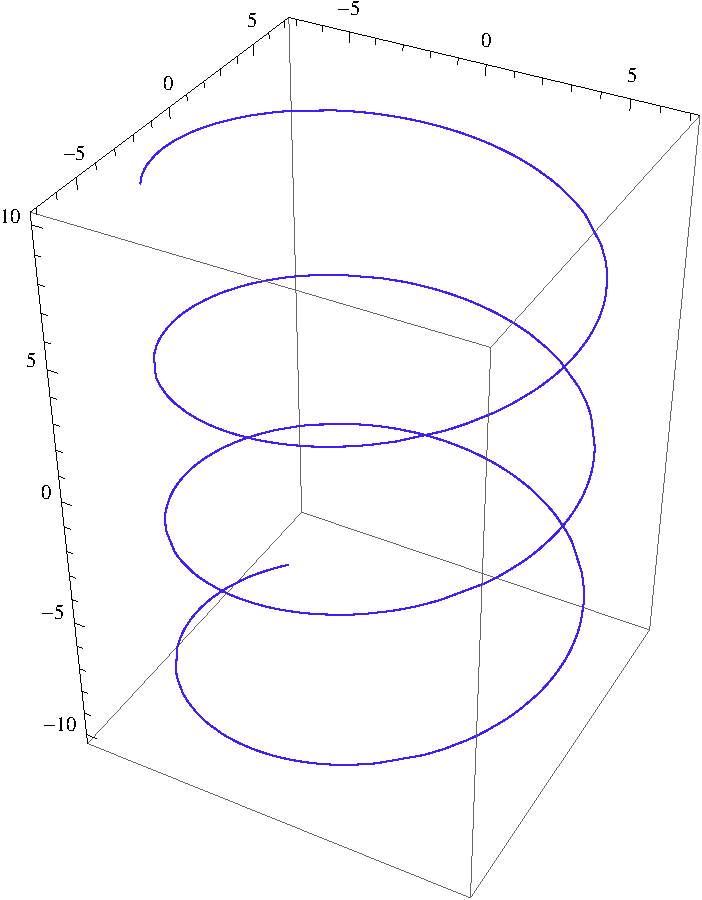
\includegraphics[height=4cm, keepaspectratio]{Bilder/Schraubenlinie.pdf}
		\caption{Schraubenlinie aus \ref{sub:55} \ref{55:enum:3})}
		}
	\end{figure}
	\item \label{55:enum:4}$\gamma : \mathds{R}\to \mathds{R}^2$, $\gamma(t)= (t- \sin t , 1 - \cos t  )$. (\hyperref[sub:511]{Zykloid})
	\begin{figure}[h]
		\centering{
		\begin{tikzpicture}[scale=0.9]
			%\draw[help lines] (0,0) grid(8,4);
			\draw[thick] (-0.4,0) -- (0,0) node[below]{$0$} -- (4,0) node[below]{$2\pi$ } --  (8,0) node[below]{$4\pi$ }-- (8.4,0);
			\draw[thick] (0,-0.2) -- (0,2) node[left]{$1$}-- (0,3);
			\draw[ultra thick, IndianRed3] (4,0) arc (0:180:2) ;
			\draw[ultra thick, IndianRed3] (8,0) arc(0:180:2);
		\end{tikzpicture}
		\caption{Graph der Kurve aus \ref{sub:55} \ref{55:enum:4}) (Zykloid)}
		}
	\end{figure}
\end{enumerate}
% subsection 55 (end)

\subsection[Definition Rektifizierbarkeit]{Definition} % (fold)
\label{sub:56}
Eine Kurve $\gamma : [a,b] \to \mathds{R}^n$ heißt \Index{rektifizierbar} mit der Länge $L$, falls gilt: Für jedes $\varepsilon >0$ existiert $\delta >0$ mit folgender 
Eigenschaft: Für jede Unterteilung $a= t_0 < t_1 < \ldots < t_n = b$ mit $\abs*{t_j - t_{j-1}}< \delta  $ für $j=1, \ldots ,n$  gilt:
\[
	 \Bigg| \underbrace{\sum_{j=1}^{n}  \norm[2]{\gamma(t_j) - \gamma(t_{j-1})}}_{\text{Länge des Polygonzugs}} - L \Bigg| < \varepsilon 
\]
\begin{figure}[ht]
	\centering{
	\begin{tikzpicture}[xscale=0.7, yscale=0.5]
		%\draw[help lines] (0,0) grid (8,4);
		\coordinate (a) at (0,0);
		\coordinate (b) at (1,2);
		\coordinate (c) at (3,3);
		\coordinate (d) at (5,1);
		\coordinate (f) at (6,1);
		\coordinate (g) at (7,4);
		\draw[ultra thick] (a) to (b) to (c) to (d) to (f) to (g);
		\draw[ultra thick, Tomato3] (a) to [out=80, in=220](b) to [out=40, in=180](c) to [out=0, in=120](d) to [out=-60, in=220](f) to [out=30, in=-90](g);
		\node[right, Tomato3] at (7,2.7) {$\gamma$};
		\draw[fill, DodgerBlue3] (a) circle[radius=0.07] node[below]{$\gamma(a)$};
		\draw[fill, DodgerBlue3] (g) circle[radius=0.07] node[above]{$\gamma(b)$};
		\draw[fill, Chartreuse4] (b) circle[radius=0.07] node[above left]{$\gamma(t_1)$};
		\draw[fill, Chartreuse4] (c) circle[radius=0.07] node[above]{$\gamma(t_2)$};
		\draw[fill, Chartreuse4] (d) circle[radius=0.07] node[below left]{$\gamma(t_3)$};
		\draw[fill, Chartreuse4] (f) circle[radius=0.07] node[below right]{$\gamma(t_4)$};
	\end{tikzpicture}
	\caption{Polygonzug für ein rektifizierbares $\gamma$}
	}
\end{figure}
% subsection 56 (end)

\subsection[Bemerkung über Stetigkeit und Rektifizierbarkeit]{Bemerkung} % (fold)
\label{sub:57}
$\gamma$ stetig $\not\Rightarrow \gamma$ rektifizierbar
% subsection 57 (end)

\subsection[Lemma über stetig differenzierbare Kurven]{Lemma} % (fold)
\label{sub:58}
Sei $\gamma : [a,b] \to \mathds{R}^n$ stetig differenzierbar. Zu $\varepsilon >0 $ existiert $\delta >0$ sodass für alle $\overline{t} \not= t \in [a,b] $ mit
$\abs*{\overline{t} - t }< \delta  $, gilt 
\[
	\norm[2]{\frac{1}{\overline{t}- t } \big(\gamma(\overline{t} ) - \gamma(t)\big) - \gamma'(\overline{t} ) } < \varepsilon 
\]
\minisec{Beweis}
Für $i \in \{1, \ldots ,n \}$ ist $\gamma'_i : [a,b] \to \mathds{R}$ stetig, nach Satz \ref{sub:413} also gleichmäßig stetig. D.h. 
$\forall \varepsilon >0 \, \exists \delta_i >0 : \text{ für } s,\overline{t} \in [a,b] \text{ mit } \abs*{s- \overline{t} }< \delta_i  $ gilt: 
$\abs*{\gamma'_i (s) - \gamma'_i (\overline{t})} < \frac{\varepsilon}{\sqrt{n}}  $. Setze nun: $\delta := \min \{\delta_i, \ldots , \delta_n \} >0$. Für 
$\overline{t} \not= t$ mit $\abs*{\overline{t}  -t }< \delta  $ existiert nach dem Mittelwertsatz ein $s_i$ zwischen $\overline{t} $ und $t$ mit 
\[
	\gamma'_i (s_i) = \frac{\gamma_i (\overline{t} ) - \gamma_i(t)}{\overline{t} -t } 
\]
Dann 
\begin{align*}
	\norm[2]{\frac{1}{\overline{t}-t } \big(\gamma(\overline{t} ) - \gamma(t)\big) - \gamma'(\overline{t} ) } &\le \sqrt{n} \cdot \max\limits_{i \in \{1, \ldots ,n\} } 
	\abs*{\frac{1}{\overline{t}-t } \big(\gamma_i(\overline{t} ) - \gamma_i(t)\big) - \gamma_i'(\overline{t} ) } \\
	&=  \sqrt{n} \cdot   \max\limits_{i \in \{1, \ldots ,n\} }  \abs*{\gamma'_i (s_i) - \gamma'_i (\overline{t} )} \\
	&\le \sqrt{n} \cdot   \frac{\varepsilon}{\sqrt{n}  } \tag{weil $\abs*{s_i- \overline{t} }< \delta < \delta_i $}   \\
	&= \varepsilon \bewende
\end{align*}
% subsection 58 (end)

\subsection[Satz über Rektifizierbarkeit]{Satz} % (fold)
\label{sub:59}
Sei $\gamma : [a,b] \to \mathds{R}^n$ stetig differenzierbar. Dann ist $\gamma$ rektifizierbar mit der Länge 
\[
	L = \int_{a} ^{b} \! \norm[2]{\gamma'(t)}  \, \mathrm{d}t 
\]
\minisec{Beweis}
Sei $\varepsilon >0$ gegeben. Wir wollen $\delta >0$, so dass für $a= t_0< \ldots < t_k =b$ mit $\abs*{t_j - t_{j-1}}< \delta  $ gilt
\[
	\abs*{ \sum_{j=1}^{k}  \norm[2]{\gamma (t_j) - \gamma (t_{j-1})}  - \int_{a} ^{b} \! \norm[2]{\gamma'(t)}  \, \mathrm{d}t } < \varepsilon
\]
Nach \ref{sub:58} gibt es $\delta_1 >0$ sodass für $a= t_0< \ldots < t_k =b$ mit  $\abs*{t_j - t_{j-1}}< \delta_1$ gilt:
\[
	\norm[2]{\frac{1}{t_j - t_{j-1}} \big( \gamma(t_j) - \gamma(t_{j-1}) \big) - \gamma'(t_j)  } < \frac{\varepsilon}{2 \abs*{b-a} }  
\]
\[
	\Rightarrow \abs*{\norm[2]{ \gamma(t_j) - \gamma(t_{j-1}) } - \norm[2]{\gamma'(t_j)}  \cdot  \abs*{ t_j - t_{j-1}}}  < \frac{\varepsilon}{2 \abs*{b-a} } \cdot 
	\abs*{t_j - t_{j-1}} \tag{$\star$}
\]   
Da $f : t \mapsto \norm[2]{\gamma'(t)} $ gleichmäßig stetig ist, existiert $\delta_2 >0$ sodass für $a= t_0< \ldots < t_k =b$ mit  $\abs*{t_j - t_{j-1}}< \delta_2$ gilt:
\[
	\norm[\infty]{ \norm[2]{\gamma'(t_1)} \cdot \mathds{1}_{[t_0, t_1]}  + \sum_{j=2}^{k}  \norm[2]{\gamma'(t_j)} \cdot \mathds{1}_{(t_{j-1},t_j]}  - f
	}  < \frac{\varepsilon}{2 \abs*{b-a} } 
\]
\[
	\Rightarrow  \abs*{\sum_{j=1}^{k}  \norm[2]{\gamma'(t_j)} \cdot \abs*{t_j - t_{j-1}} - \int_{a} ^{b} \! \norm[2]{\gamma'(t)}  \, \mathrm{d}t   } < \frac{\varepsilon}{2}
	\tag{$\star \star$} 
\]
Für $\delta := \min \{\delta_1, \delta_2\}$ gilt: Für jede Unterteilung $a= t_0< \ldots < t_k =b$ mit  $\abs*{t_j - t_{j-1}}< \delta$ gilt:
\begin{align*}
	& \abs*{ \sum_{j=1}^{k}  \norm[2]{\gamma(t_j) - \gamma(t_{j-1})} - \int_{a} ^{b} \! \norm[2]{\gamma'(t)}  \, \mathrm{d}t  }   \\
	&\le \abs*{\sum_{j=1}^{k} \norm[2]{\gamma(t_j) - \gamma(t_{j-1})}  - \sum_{j=0}^{k} \norm[2]{\gamma'(t_j)} \cdot  \abs*{t_j - t_{j-1}}    } 
	+ \abs*{\sum_{j=1}^{k}  \norm[2]{\gamma'(t_j)} \abs*{t_j - t_{j-1}} - \int_{a} ^{b} \! \norm[2]{\gamma'(t)}  \, \mathrm{d}t   } \\
	&\le \sum_{j=1}^{k}  \frac{\varepsilon}{2 \abs*{b-a} } \cdot  \abs*{t_j - t_{j-1}} + \frac{\varepsilon}{2} = \varepsilon     
\end{align*}
% subsection 59 (end)

\subsection[Parametertransformation]{Proposition und Definition} % (fold)
\label{sub:510}
Sei $\gamma : [a,b] \to \mathds{R}^n$ eine Kurve, $\varphi : [c,d] \to [a,b]$ bijektiv und stetig. Dann heißt $\varphi$ \Index{Parametertransformation} und 
$\zeta := \gamma \circ \varphi : [c,d] \to \mathds{R}^n$ ist eine Kurve. \\
Falls $\gamma, \varphi, \varphi ^{-1}$ stetig differenzierbar sind, so gilt: 
\begin{enumerate}[a)]
	\item $\varphi '(t) \not= 0$ für $t \in [c,d]$ und 
	$(\varphi ^{-1})'(t) \not= 0$ für $t \in [a,b]$
	\item $\zeta'(t) = \varphi ' (t ) \cdot \gamma ' \big( \varphi (t) \big)$ für $t \in [c,d]$ insbesondere ist $\zeta$ stetig differenzierbar.
	\item $\int_{a} ^{b} \! \norm[2]{\gamma'(t)}  \, \mathrm{d}t = \int_{c} ^{d} \! \norm[2]{\zeta'(t)}  \, \mathrm{d}t $
\end{enumerate}
\minisec{Beweis}
$\gamma \circ \varphi$ ist stetig nach Proposition \ref{sub:34}, also eine Kurve.
\begin{enumerate}[a)]
	\item $\varphi \circ  \varphi ^{-1} = \id_{[c,d]}$ und 
	\begin{align*}
		1 &= (\id_{[c,d]})' (t) = ( \varphi ^{-1} \circ  \varphi)' (t) = \enbrace*{\varphi ^{-1}}' ( \varphi(t)) \cdot \varphi'(t) \\
		&\Rightarrow \varphi'(t) \not= 0  \text{ für } t \in [c,d], \quad  \enbrace*{\varphi ^{-1}}' (t) \not= 0  \text{ analog}
	\end{align*}
	\item \begin{align*}
		\zeta'(t)= (\gamma \circ \varphi)' (t) = \big( (\gamma_1 \circ \varphi)' (t), \ldots , (\gamma_n \circ \varphi)'(t) \big) &= \Big(\varphi'(t) \cdot 
		\gamma_1'( \varphi(t)), \ldots , \varphi'(t) \cdot  \gamma'_n \big(\varphi(t) \big) \Big) \\
		&= \varphi'(t) \cdot  \enbrace*{ \gamma_1' (\varphi(t)) , \ldots , \gamma_n'(\varphi(t))} \\
		&= \varphi'(t) \cdot \gamma'(\varphi(t)) 
	\end{align*}
	\item $\varphi'(t) \not= 0$ für $t \in [c,d]$, $\varphi' $ stetig. Daraus folgt (1)$\varphi' (t ) >0$ für $t \in [c,d]$ oder (2)$\varphi'(t) < 0 $ für $t \in [c,d]$
	(nach Zwischenwertsatz). Wir betrachten (1); (2) geht analog
	
	$\varphi' (t ) >0$ für alle $t \Rightarrow \varphi$ streng monoton wachsend und $\varphi(c)=a$, $\varphi(d)=b$. Es gilt
	\begin{align*}
		\int_{c} ^{d} \! \norm[2]{ \zeta'(t)}  \, \mathrm{d}t &= \int_{c} ^{d} \! \norm[2]{\varphi'(t) \cdot  \gamma'(\varphi(t))}  \, \mathrm{d}t  
		= \int_{c} ^{d} \! \varphi'(t) \cdot  \norm[2]{\gamma'( \varphi(t))}  \, \mathrm{d}t \\
		&= \int_{\varphi(c)} ^{\varphi(d)} \! \norm[2]{\gamma'(n)}  \, \mathrm{d}n \tag{Substitution 13.17 Ana \RM{1}} \\
		&= \int_{a} ^{b} \! \norm[2]{\gamma'(t)}  \, \mathrm{d}t \bewende
	\end{align*}
\end{enumerate}
% subsection 510 (end)

\subsection[Beispiel: Länge eines Zykloids]{Beispiel} % (fold)
\label{sub:511}
Sei $\gamma(t)= (t- \sin t , 1-  \cos t  )$ ein \Index{Zykloid}. Dann gilt: $\gamma'(t) = (1- \cos t , \sin t )$ und 
\begin{align*}
	\norm[2]{\gamma'(t)}  = \enbrace*{ (1- \cos t)^2 + (\sin t)^2}^{\frac{1}{2} } &= \enbrace*{1- 2 \cos t + (\cos t)^2 + (\sin t)^2}^{\frac{1}{2}}  \\
	&= (2-2 \cos t)^{\frac{1}{2} } = ( 2 \cdot  (1- \cos t))^{\frac{1}{2}} = \enbrace*{2 \cdot 2 \sin^2 \enbrace*{\frac{t}{2}}}^{\frac{1}{2} } \\
	&= 2 \sin \enbrace*{\frac{t}{2}} \tag*{$t \in [0, 2\pi ]$}
\end{align*}
benutzt: $\cos x - \cos y = -2 \sin \frac{x+y}{2} \sin \frac{x-y}{2}  $
\begin{align*}
	L= \int_{0} ^{2 \pi } \! \norm[2]{\gamma'(t)}  \, \mathrm{d}t = 2 \int_{0} ^{2 \pi } \! \sin \enbrace*{\frac{t}{2}}   \, \mathrm{d}t \stackrel{n=\frac{t}{2} }{=} 
	4 \int_{0} ^{2 \pi } \! \sin n  \, \mathrm{d}n = 4 \big(- \cos (n) \big) \Big|_0^\pi  = 8      
\end{align*}
% subsection 511 (end)
% section 5 (end)
\newpage
\section{Abbildungen von $\mathds{R}^n$ nach $\mathds{R}$} % (fold)
\label{sec:6}
\begin{figure}[ht]
	\centering{
	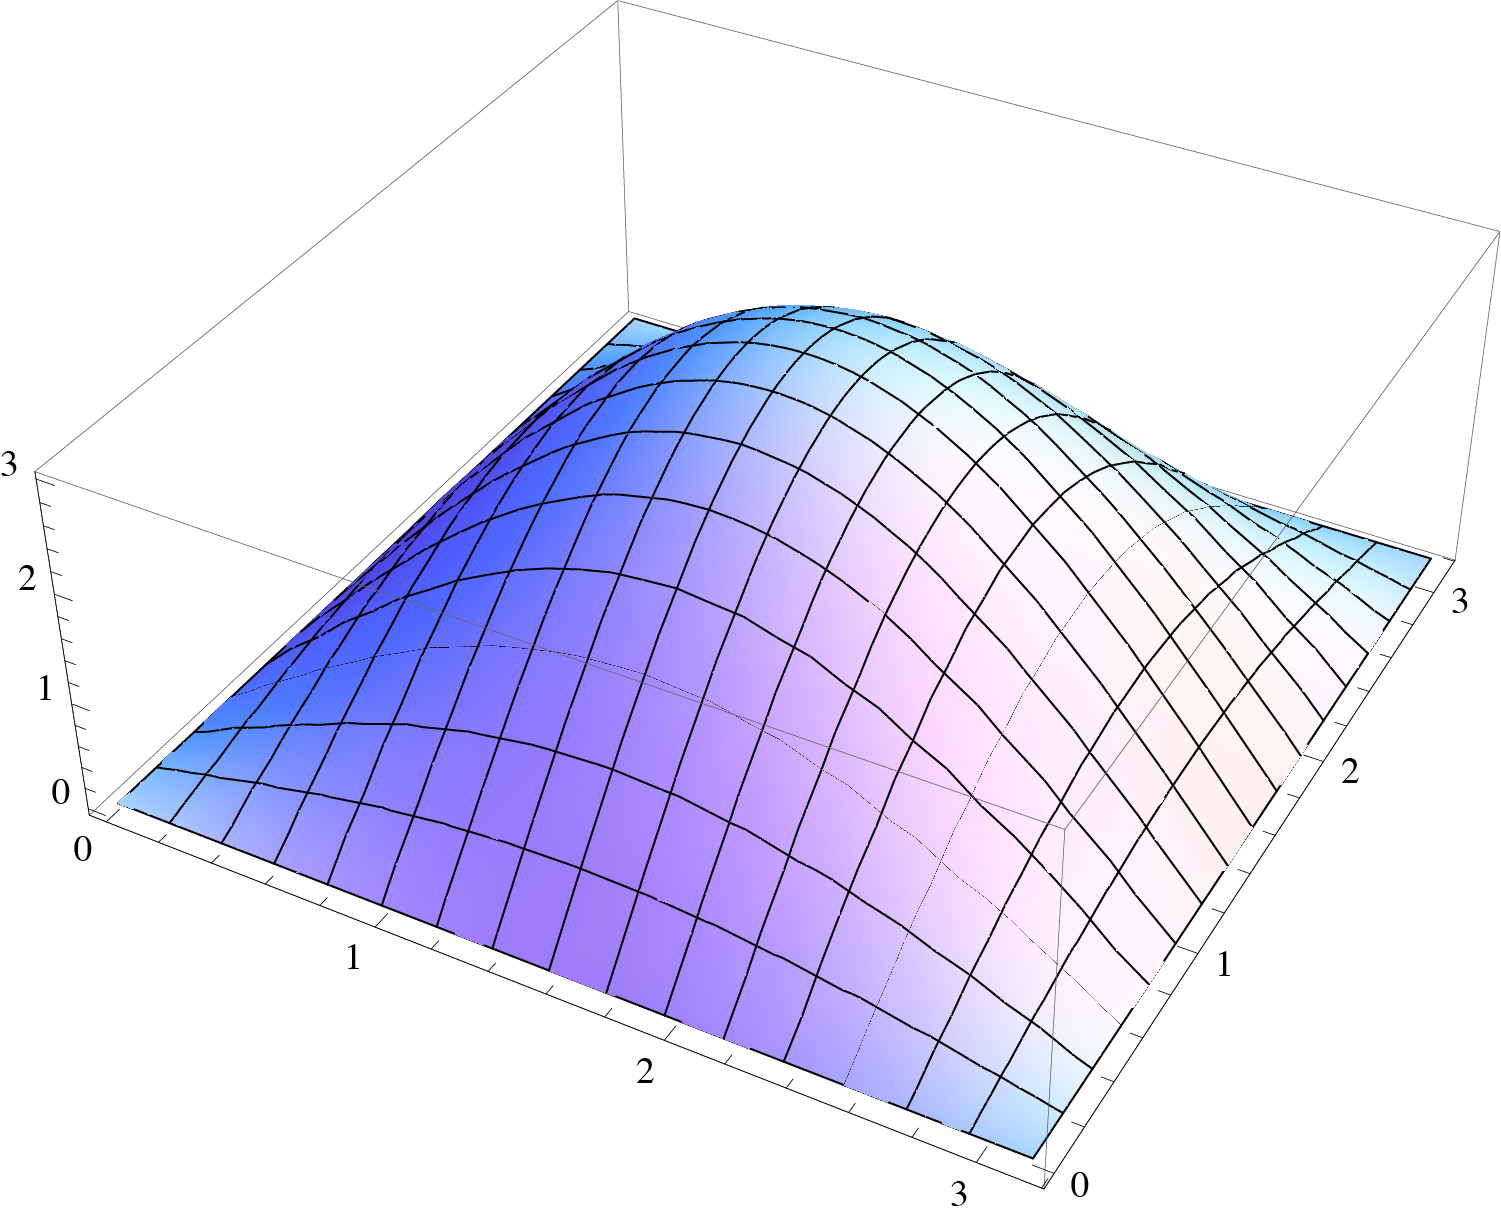
\includegraphics[height=5cm, keepaspectratio]{Bilder/rn_to_r_3d_2x.png} \qquad 
	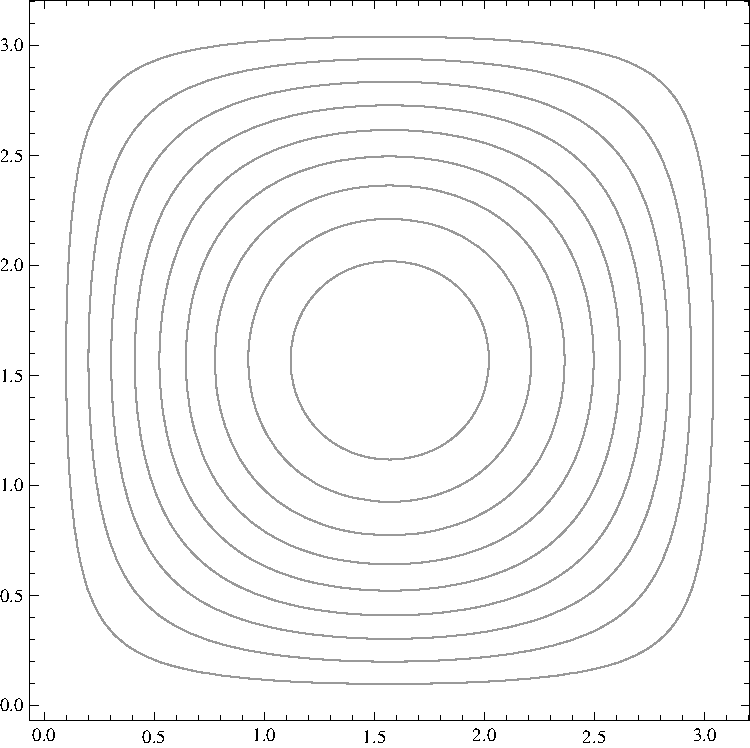
\includegraphics[width=5cm, keepaspectratio]{Bilder/rn_to_r_2d.pdf}
	\caption{Darstellung einer Abbildung $f : U \to \mathds{R}$ mit $U \subset \mathds{R}^2$ als 3D-Plot und als Niveaulinien}
	}
\end{figure}


\subsection[Definition: Partielle Differenzierbarkeit]{Definition} % (fold)
\label{sub:61}
Sei $U \subset \mathds{R}^n$ und $f : U \to \mathds{R}$ eine Abbildung. 
\begin{enumerate}[a)]
	\item Für $\underline{x} \in U $, $i \in \set{1,\ldots,n}$ heißt $f$ \Index{partiell differenzierbar} in $\underline{x} $ bezüglich der $i$-ten Koordinate, falls gilt:
	\begin{enumerate}[(i)]
		\item Es gibt eine Folge $(h_k)_{k \in \mathds{N}} \subset \mathds{R}^*$ mit $\lim_{ k \to \infty} h_k = 0$ und $\underline{x} + h_k \cdot \underline{e}_i \in U $,
		wobei $k \in \mathds{N}$
		\item Der Limes 
		\[
			D_i f(\underline{x}) := \lim_{ \substack{h \to 0, h \not= 0 \\ \underline{x} + h \underline{e}_i \in U  }}  \frac{f( \underline{x} + h \cdot\underline{e}_i) - 
			f(\underline{x} )}{h} \in \mathds{R}
		\]
		existiert. (Dabei ist $\underline{e}_i = ( 0, \ldots , \stackrel{i}{1}, \ldots , 0)$). Wir schreiben auch $\frac{\partial f}{\partial x_i} $ für $D_i f$.
	\end{enumerate}
	\item $f$ heißt partiell differenzierbar, falls $f$ für jedes $\underline{x} \in U $ und jedes $i \in \set{1, \ldots , n} $ partiell differenzierbar in $\underline{x} $
	bezüglich der $i$-ten Koordinate ist.
	
	$f$ heißt stetig partiell differenzierbar, falls außerdem $D_i f : U  \to \mathds{R}$ stetig ist für jedes $i \in \set{1, \ldots , n} $
\end{enumerate}
Der \Index{Gradient} von $f$ in $\underline{x}$ ist 
\[
	\grad f(\underline{x}) = \enbrace*{ D_1 f(\underline{x}), \ldots , D_n f(\underline{x}) } \in \mathds{R}^n 
\]
Wir schreiben auch $\nabla f(\underline{x})$ für $\grad f(\underline{x} )$.
% subsection 61 (end)

\subsection[Bemerkung zur partiellen Differenzierbarkeit]{Bemerkung} % (fold)
\label{sub:62}
\begin{enumerate}[(i)]
	\item Die Bedingung \ref{sub:61} (a)(i) ist automatisch erfüllt, falls $U \subset \mathds{R}^n$ offen ist. \hfill (warum?)
	\item Für $\underline{x}= (x_1, \ldots , x_n) $ definiere $f_i : U_i \to \mathds{R}$ durch $f_i(\xi) = f \enbrace*{ (x_1, \ldots , \xi, \ldots , x_n)} $, wo 
	\[
		U_i := U \cap \underbrace{\set[(x_1, \ldots , \xi, \ldots , x_n)]{\xi \in \mathds{R}}}_{\sim \mathds{R}}  \subset \mathds{R}^n
	\]
	Es gilt
	\[
		D_i f (\underline{x} ) =  \lim_{ h \to 0, h \not= 0} \frac{f_i (x_i +h) - f_i(x_i)}{h}  = f_i' (x_i)
	\]
\end{enumerate}
% subsection 62 (end)

\subsection[Definition: Vektorfeld und Divergenz]{Definition} % (fold)
\label{sub:63}
Ein \Index{Vektorfeld} auf $U \subset \mathds{R}^n$ ist eine Abbildung $\underline{v} : U \to \mathds{R}^n $. $\underline{v} $ heißt partiell differenzierbar, wenn alle
Komponenten $v_1, \ldots , v_n : U \to \mathds{R}$ partiell differenzierbar sind. In diesem Fall heißt 
\[
	\dive \underline{v} := \sum_{i=1}^{n} \frac{\partial v_i}{\partial x_i}   
\]
\Index{Divergenz} von $\underline{v}$ in $\underline{x}$. Wir schreiben auch 
\[
	\dive \underline{v} = \sprod{\nabla}{\underline{v} } =   \sprod{\begin{pmatrix}
		\frac{\partial}{\partial x_1} \\
		\vdots \\
		\frac{\partial}{\partial x_n} 
	\end{pmatrix}}{\begin{pmatrix}
		v_1 \\
		\vdots \\
		v_n
	\end{pmatrix}} 
\]
% subsection 63 (end)

\subsection[Beispiele zum partiellen Differenzieren]{Beispiel} % (fold)
\label{sub:64}
\begin{enumerate}[(i)]
	\item Betrachte $r : \mathds{R}^n \to \mathds{R}$ mit $r(\underline{x}) := \norm[2]{\underline{x}}$. Niveaumengen sind 
$N_r(c) := \set[\underline{x} \in \mathds{R}^n ]{r(\underline{x})= c} $ für $c >0$ also \Index{Sphären} mit Radius $c$. 

$r$ ist auf $\mathds{R}^n \setminus \{0\} := U$ stetig partiell differenzierbar: Für $0 \not= \underline{x} = (x_1, \ldots , x_n)$ definiere $r_i : U_i \to \mathds{R}$
durch $r_i ( \xi) := r((x_1, \ldots , x_{i-1}, \xi, x_{i+1}, \ldots , x_n)) = (x_1^2 + \ldots +  x_{i-1}^2 + \xi^2 + x_{i+1}^2 + \ldots + x_n^2)^{\frac{1}{2}}$ Dann ist
\begin{align*}
	D_i r(\underline{x}) = \frac{\partial r}{\partial x_i} ( \underline{x} ) = r_i' (x_i) 
	= 2 x_i \cdot \frac{1}{2} \cdot  (x_1^2, \ldots , x_{i-1}^2, x_i^2, x_{i+1}^2, \ldots , x_n^2)^{-\frac{1}{2}} = \frac{x_i}{r(\underline{x})} 
\end{align*}
\item Sei $r$ wie oben und $f : \mathds{R}_+^* \to \mathds{R}$ differenzierbar. Dann ist $f \circ r : \mathds{R}^n \setminus \{0\} \to \mathds{R}$ partiell differenzierbar.
Es gilt 
\begin{align*}
	\frac{\partial}{\partial x_i} (f \circ r) ( \underline{x} ) = f'(r(\underline{x})) \frac{\partial r}{\partial x_i} (\underline{x} )  = f'( r(\underline{x} )) \cdot 
	\frac{x_i}{r(\underline{x} )} 
\end{align*}
\item Sei $n \ge 2$. Definiere $g : \mathds{R}^n \to \mathds{R}$ durch 
\[
	g( \underline{x}) := \begin{cases}
		\frac{(x_1 \cdot x_2 \cdot \ldots \cdot x_n)  =: e}{r(\underline{x})^{2n} =: \frac{1}{d} } , &\text{ falls }\underline{x} \not= 0 \\
		0 , &\text{ falls } \underline{x} = 0 
	\end{cases}
\]
$g$ ist auf $\mathds{R}^n \setminus \{0\}$ partiell differenzierbar mit (Produktregel)
\[
	\frac{\partial g}{\partial x_i}( \underline{x} ) =  x_1 \cdot x_2 \cdot \ldots \cdot x_{i-1} \cdot x_{i+1} \cdot \ldots \cdot x_n \cdot r(\underline{x} )^{-2n}
	+ x_1 \cdot x_2 \cdot \ldots \cdot x_n \cdot r(\underline{x} )^{-2n-1} \cdot \frac{x_i}{r(\underline{x} )} \cdot (-2n)
\]
$g$ ist in $0$ partiell differenzierbar:
\[
	\frac{\partial g}{\partial x_i}(0) = \lim_{ h \to 0, h \not= 0} \frac{g(0+ h \cdot \underline{e}_i ) - g(0)}{h}  = 0
\]
D.h. $g$ ist auf $\mathds{R}^n$ partiell differenzierbar. Aber $g$ ist nicht stetig in $0$: Es gilt 
$  \mathds{R}^n \ni\enbrace*{\frac{1}{k}, \ldots , \frac{1}{k}}  \xrightarrow{k \to \infty} 0$ aber 
\[
	g \enbrace*{ \enbrace*{\frac{1}{k}, \ldots , \frac{1}{k}} }  = \frac{\frac{1}{k^n} }{\enbrace*{\enbrace*{n \cdot \frac{1}{k^2}}^{\frac{1}{2}} }^{2n} } 
	= \frac{ \frac{1}{k^n}}{n^n \cdot  \frac{1}{k^{2n}} } = \enbrace*{\frac{k}{n} }^n \xrightarrow{k \to \infty} \infty   
\]
D.h. partielle Differenzierbarkeit impliziert nicht Stetigkeit.
\item \label{64:enum:4} Sei $U \subset \mathds{R}^n$, $f  : U \to \mathds{R}$ partiell differenzierbar, dann ist $\grad f : U \to \mathds{R}^n$ ein Vektorfeld.

Es gilt \marginnote{Jeder Vektor wird also normiert/zu einem Einheitsvektor}
\[
	\grad r(\underline{x}) = \enbrace*{ \frac{\partial r}{ \partial x_1}(\underline{x} ) , \ldots , \frac{\partial r}{ \partial x_n}(\underline{x} )} =
	\enbrace*{ \frac{x_1}{r(\underline{x})} , \ldots , \frac{x_n}{r(\underline{x} )}  } = \frac{1}{r(\underline{x} )} \cdot \underline{x}  
\]
\begin{figure}[ht]
	\centering{
	\begin{tikzpicture}[scale=0.8]
		\draw[->, thick] (-2,0) -- (2,0);
		\draw[->, thick] (0,-2) -- (0,2); 
		\draw[->, ultra thick, Salmon2](20:0.8) -- (20:1.8);
		\draw[->, ultra thick, Salmon2](257:0.4) -- (257:1.4);
		\draw[->, ultra thick, Salmon2](67:0.3) -- (67:1.3);
		\draw[->, ultra thick, Salmon2](110:0.2) -- (110:1.2);
		\draw[->, ultra thick, Salmon2](340:1) -- (340:2);
		\draw[->, ultra thick, Salmon2](160:0.1) -- (160:1.1);
		\draw[->, ultra thick, Salmon2](230:0.3) -- (230:1.3);
		\draw[->, ultra thick, Salmon2](300:1) -- (300:2);
		\draw[->, ultra thick, Salmon2](2001:0.9) -- (200:1.9);
		\draw[->, ultra thick, Salmon2](320:0.2) -- (320:1.2);
		\draw[->, ultra thick, Salmon2](128:1) -- (128:2);
		\draw[->, ultra thick, Salmon2](42:1.1) -- (42:2.1);
	\end{tikzpicture}
	\caption{Vektorfeld aus \ref{sub:64}(\ref{64:enum:4}) (Man beachte, dass alle Vektoren Einheitsvektoren sind)}
	}
\end{figure}
\item 
\begin{align*}
	\dive ( \grad r) (\underline{x}) = \dive \enbrace*{ \frac{1}{r(\underline{x} )} \cdot \underline{x}  } &= \sum_{i=1}^{n} \frac{\partial }{\partial x_i} 
	\enbrace*{\frac{1}{r(\underline{x} )} \cdot x_i }  \\ &=   \sum_{i=1}^{n} \enbrace*{ \enbrace*{\frac{\partial }{\partial x_i} \frac{1}{r(\underline{x})}} \cdot x_i +
	\frac{1}{r (\underline{x} )} \cdot 1  } \tag{Produktregel}\\
	&= \enbrace*{\sum_{i=1}^{n} - \frac{1}{r(\underline{x})^2} \cdot \frac{x_i}{r(\underline{x})} \cdot x_i  } + \frac{n}{r(\underline{x} )} \tag{Kettenregel}\\
	&= - \frac{1}{r(\underline{x} )} \cdot \underbrace{\frac{\sum_{i=1}^{n} x_i^2}{r(\underline{x} )^2}}_{=1}  + \frac{n}{r(\underline{x} )} = (n-1) \cdot \frac{1}{r(\underline{x} )}   
\end{align*}
Formaler (vgl. mit Produktregel): 
\[
	\sprod{\nabla}{ \frac{1}{r(\underline{x} )} \cdot \underline{x}  } = \dive \enbrace*{\frac{1}{r(\underline{x} )} \cdot  \underline{x}} = \sprod{\nabla 
	\frac{1}{r(\underline{x})} }{\underline{x} } + \frac{1}{r(\underline{x})} \cdot \underbrace{\sprod{\nabla}{\underline{x}}}_{=n}
\]
Allgemeiner: $\sprod{\nabla}{f \cdot \underline{v} } = \sprod{\nabla f}{\underline{v} } + f \sprod{\nabla}{\underline{v}}   $
\end{enumerate}
% subsection 64 (end)

\subsection[Definition: $k$-mal partiell differenzierbar]{Definition} % (fold)
\label{sub:65}
Sei $U \subset \mathds{R}^n$ und $f : U \to \mathds{R}$ partiell differenzierbar. $f$ heißt zweimal partiell differenzierbar, falls alle partiellen Ableitungen 
$D_i f : U \to \mathds{R}$ wieder partiell differenzierbar sind. Induktiv definieren wir: $f$ heißt $(k+1)$ mal partiell differenzierbar, falls $f$ $k$-mal partiell
differenzierbar ist und alle partiellen Ableitungen $k$-ter Ordnung 
\[
	D_{i_k} \ldots D_{i_2}D_{i_1} f : U \to \mathds{R}
\]
partiell differenzierbar sind. $f$ heißt $k$-mal stetig partiell differenzierbar, falls $f$ $k$-mal partiell differenzierbar ist und alle partiellen Ableitungen der 
Ordung $\le k$ stetig sind. Wir schreiben auch 
\begin{align*}
	D_{i_k} \ldots D_{i_1} f &= \frac{\partial^k f}{\partial x_{i_k} \cdot \ldots  \cdot \partial x_{i_2} \cdot \partial x_{i_1}}  \\
	D_i D_i f &= D_i^2 f = \frac{\partial^2 f}{\partial x_i^2} 
\end{align*}
% subsection 65 (end)

\subsection[Satz über Reihenfolge des Differenzierens]{Satz} % (fold)
\label{sub:66}
Sei $U \subset \mathds{R}^n$ offen und $f : U \to \mathds{R}$ zweimal stetig partiell differenzierbar. Dann gilt für $\underline{a} \in U $, $i,j \in \{1, \ldots ,n\}$
\[
	D_i D_j f (\underline{a}) =  D_j D_i f(\underline{a})
\]
\minisec{Beweis}
O.E. sei $n=2$, $i=1$ und $j=2$ (warum?). Aus $U \subset \mathds{R}^2$ offen folgt: Es existiert ein $\delta >0$ mit 
$[a_1 - \delta , a_1 + \delta ] \times [a_2 - \delta , a_2 + \delta ] \subset U$. Betrachte $(\overline{x}_1, \overline{x}_2) \in  [a_1 - \delta , a_1 + \delta ] \times 
[a_2 - \delta , a_2 + \delta ] $ mit $\overline{x}_1 \not=a_1 , \overline{x}_2 \not= a_2$. Definiere
\[
	F: [a_1 - \delta , a_1 + \delta ] \to \mathds{R} \enspace \text{ durch } F(x_1) := f \enbrace*{ (x_1, \overline{x}_2 )} - f \enbrace*{(x_1, a_2)}  
\]
$F$ ist stetig differenzierbar, da $f$ stetig differenzierbar ist. Nach dem Mittelwertsatz existiert $\xi$ zwischen $\overline{x}_1 $ und $a_1$ mit 
\[
	 f(\overline{x}_1, \overline{x}_2 ) - f(\overline{x}_1, a_2 ) - \enbrace*{ f(a_1, \overline{x}_2 ) - f (a_1, a_2)} = F(\overline{x}_1 ) - F(a_1) = 
	 (\overline{x}_1 - a_1 ) \cdot F'(\xi) = (\overline{x}_1 - a_1 ) ( D_1 f(\xi, \overline{x}_2 ) - D_1 f(\xi, a_2) )
\]
Definiere $G : [a_2 - \delta , a_2 + \delta ] \to \mathds{R}$ durch $G(x_2) := D_1 f (\xi, x_2)$. $G$ ist stetig differenzierbar. Nach dem Mittelwertsatz existiert
$\eta$ zwischen $\overline{x}_2 $ und $a_2$ mit 
\begin{gather*}
	D_1 f(\xi, \overline{x}_2 ) - D_1 f(\xi, a_2) = G(\overline{x}_2 ) - G(a_2) = (\overline{x}_2 - a_2 ) \cdot G'(\eta) = (\overline{x}_2 - a_2) \cdot D_2 D_1 f(\xi, \eta)
\end{gather*}
Es folgt 
\begin{align*}
	f(\overline{x}_1, \overline{x}_2 ) - f(\overline{x}_1, a_2 ) - f(a_1, \overline{x}_2 ) + f(a_1, a_2) = (\overline{x}_1 - a_1 ) \cdot ( \overline{x}_2 - a_2 ) \cdot  
	D_2 D_1 f(\xi, \eta) \tag{$\star$}
\end{align*}
Definiere nun $\tilde F : [a_2 - \delta , a_2 + \delta ] \to \mathds{R}$ durch $\tilde F (x_2) := f (\overline{x}_1, x_2 ) - f(a_1, x_2)$. Dann ist $\tilde F$ stetig 
differenzierbar. Nach dem Mittelwertsatz existiert ein $\tilde \eta$ zwischen $\overline{x}_2 $ und $a_2$ mit 
\begin{gather*}
	\qquad \qquad \tilde F (\overline{x}_2 ) - \tilde F (a_2) = (\overline{x}_2 -a_2 ) \cdot \tilde F'{\tilde \eta} \\
	f(\overline{x}_1 , \overline{x}_2  ) - f(a_1, \overline{x}_2 ) - \enbrace*{ f(\overline{x}_1 - a_2 ) - f(a_1, a_2)} =\qquad \qquad \qquad 
	= (\overline{x}_2 - a_2 ) (D_2 f(\overline{x}_1, \tilde \eta ) - D_2 f(a_2, \tilde \eta))
\end{gather*}
Definiere $\tilde G : [a_1 - \delta , a_1 + \delta ]\to \mathds{R}$ durch $\tilde G(x_1) := D_2 f(x_1, \tilde \eta)$. $\tilde G$ ist stetig differenzierbar. Nach dem 
Mittelwertsatz existiert $\tilde \xi$ zwischen $a_1$ und $\overline{x}_1 $ mit:
\[
	D_2 f(\overline{x}_1 , \tilde \eta ) - D_2 f(a_1, \tilde \eta)= \tilde G (\overline{x}_1 ) - \tilde G(a_1) = (\overline{x}_1 -a_1 )  \tilde G \left( \tilde \xi \right)
	= (\overline{x}_1 - a_1 ) \cdot D_1 D_2 f \left(\tilde \xi, \tilde \eta \right)
\]
Es folgt 
\[
	f(\overline{x}_1, \overline{x}_2  ) - f (a_1, \overline{x}_2 ) - f(\overline{x}_1, a_2 ) + f(a_1, a_2) = (\overline{x}_1 - a_1 ) ( \overline{x}_2 -a_2 ) D_1 D_2 f
	\enbrace*{\tilde \xi , \tilde \eta} 
\]
$\stackrel{(\star)}{\Longrightarrow}   D_1 D_2 f \enbrace*{\tilde \xi, \tilde \eta} = D_2 D_1 f( \xi, \eta) $
\begin{align*}
	D_1 D_2 f \enbrace*{\tilde \xi, \tilde \eta} &\xrightarrow{\substack{\overline{x}_1 \to a_1 \\ \overline{x}_2  \to a_2  }} D_1 D_2 f(a_1, a_2) \\
	D_2 D_1 f( \xi, \eta) &\xrightarrow{\substack{\overline{x}_1 \to a_1 \\ \overline{x}_2  \to a_2  }} D_2 D_1 f(a_1, a_2)
\end{align*}
wegen Stetigkeit von $D_1 D_2 f$ und $D_2 D_1 f$. \bewende 
% subsection 66 (end)

\subsection{Beispiele} % (fold)
\label{sub:67}
\begin{enumerate}[(i)]
	\item Sei $U \subset \mathds{R}^3$, $\underline{v} : U \to \mathds{R}^3 $ ein partiell differenzierbares Vektorfeld. Wir definieren ein Vektorfeld 
	\[
		\rot \underline{v} := \enbrace*{ \frac{\partial v_3}{\partial x_2} - \frac{\partial v_2}{\partial x_3} , \frac{\partial v_1}{\partial x_3} - 
		\frac{\partial v_3}{\partial x_1} ,  \frac{\partial v_2}{\partial x_1} - \frac{\partial v_1}{\partial x_2}      }  \tag{Rotation von $\underline{v}$}
	\]
	Wir schreiben auch \marginnote{eventuell kennt man das Kreuzprodukt noch aus der Schule}
	\[
		\rot \underline{v} = \nabla \times \underline{v}  = \begin{pmatrix}
			\frac{\partial}{\partial x_1} \\ \frac{\partial}{\partial x_2} \\ \frac{\partial}{\partial x_3}    
		\end{pmatrix} \times \begin{pmatrix}
			v_1 \\ v_2 \\v_3
		\end{pmatrix}
	\]
	Falls $f : U \to \mathds{R}$ zweimal stetig partiell differenzierbar ist, so gilt 
	\[
		 \rot (\grad f) = \nabla \times \nabla f = \begin{pmatrix}
			\frac{\partial}{\partial x_1} \\ \frac{\partial}{\partial x_2} \\ \frac{\partial}{\partial x_3}    
		\end{pmatrix} \times \begin{pmatrix}
			\frac{\partial f}{\partial x_1} \\ \frac{\partial f}{\partial x_2} \\ \frac{\partial f}{\partial x_3}    
		\end{pmatrix} = \enbrace*{\frac{\partial^2 f}{\partial x_2 \partial x_3} - \frac{\partial^2 f}{\partial x_3 \partial x_2}, \, \ldots \, , \, \ldots   } = 0
	\]
	nach Satz \ref{sub:66}
	\item Sei $U \subset \mathds{R}^n$, $f : U \to \mathds{R}$ zweimal stetig partiell differenzierbar. Setze 
	\begin{align*}
		\Delta f := \dive \grad f =  \frac{\partial^2 f}{\partial x_1^2} + \ldots  + \frac{\partial^2 f}{ \partial x_n^2}  
	\end{align*}
	$\Delta =  \frac{\partial^2 }{\partial x_1^2} + \ldots  + \frac{\partial^2 }{ \partial x_n^2}$ heißt \Index{Laplaceoperator}. 
	
	Sei $h : \mathds{R}^n \times \mathds{R}_+ \to \mathds{R}$ eine zeitabhängige Temperaturverteilung, d.h. $h(x_1, \ldots , x_n, t)$ ist Temperatur in 
	$(x_1, \ldots , x_n)$ zum Zeitpunkt $t$. Dann erfüllt $h$ die Wärmeleitungsgleichung
	\[
		\Delta h - \lambda \cdot \frac{\partial h}{\partial t} = 0 
	\]
	mit $\frac{1}{\lambda } $ Wärmeleitfähigkeit.
\end{enumerate}
% subsection 67 (end)
% section 6 (end)
\newpage
\section{Abbildungen von $\mathds{R}^m$ nach $\mathds{R}^n$: Differenzierbarkeit} % (fold)
\label{sec:7}

\subsection[Definition: Differenzierbarkeit, Differential, Jacobimatrix]{Definition} % (fold)
\label{sub:71}
Sei $U  \subset \mathds{R}^m$ offen, $f : U \to \mathds{R}^n$ eine Abbildung.
\begin{enumerate}[(i)]
	\item $f$ heißt differenzierbar in $\underline{x} \in U$, falls gilt: Es gibt $A : \mathds{R}^m \to \mathds{R}^n$ linear und $\varphi : \mathds{R}^m \to \mathds{R}^n$
	mit 
	\[
		\boxed{f(\underline{x} + \underline{\xi}) = f(\underline{x} ) + A (\underline{\xi}) + \varphi (\underline{\xi})} 
	\]
	für alle $\underline{\xi}$ in einer Umgebung von $0$ und mit
	\[
		\lim_{ \underline{\xi} \to 0, \underline{\xi} \not= 0} \frac{1}{\norm[2]{\underline{\xi}} } \varphi (\underline{\xi}) = 0
		 \marginnote{d.h. $\varphi (\underline{\xi})$ geht \glqq schneller\grqq gegen $0$ als $\norm[2]{\underline{\xi}} $}
	\]
	Es genügt, wenn das $\varphi$ in einer Umgebung von $0$ definiert ist. \hfill (warum?)
	\item $f$ heißt differenzierbar , falls $f$ in jedem Punkt $\underline{x} \in U$ differenzierbar ist.
	\item $A (= A(\underline{x}))$ heißt \Index{Ableitung} oder \Index{Differential} von $f$ in $\underline{x}$, oft schreiben wir auch $D f(x)$. 
	
	Wir werden gleich sehen, dass $A$ nicht von der Wahl von $\varphi$ abhängt.
\end{enumerate}
Die zugehörige Matrix $(a_{ij}) \in M_{n \times m}(\mathds{R})$ heißt auch \Index{Jacobimatrix} oder \Index{Funktionalmatrix}.  
% subsection 71 (end)

\subsection[Bemerkung: Vergleich der Differenzierbarkeits-Begriffe]{Bemerkung} % (fold)
\label{sub:72}
Sei $U \subset \mathds{R}$ offen, $f : U \to \mathds{R}$, $\overline{x} \in U$. Nach Analysis \RM{1} 12.2 (iv) gilt: $f$ ist differenzierbar in $\overline{x} \in U$ (im
Sinne von Analysis \RM{1}) $\iff \exists \psi : U  \to \mathds{R}$ stetig in $\overline{x}$ mit 
\[
	f(\overline{x} + \xi) = f(\overline{x} ) + \xi \cdot \psi( \overline{x} + \xi) = f(\overline{x} ) + \underbrace{\psi (\overline{x} )}_{f'(\overline{x} )} \xi + 
	\underbrace{ \big(\psi (\overline{x} + \xi) - \psi (\overline{x} )\big) \xi}_{=: \varphi(\xi)}
\]
\[
	\lim_{ \xi \to 0, \xi \not= 0} \abs*{\frac{1}{\abs*{\xi} } \varphi (\xi) }  = \lim_{ \xi \to 0, \xi \not= 0} \abs*{\psi (\overline{x} + \xi) - \psi (\overline{x} )}
	\stackrel{\text{$\psi$ stetig in $\overline{x} $}}{=} 0
\]
$\Rightarrow f$ ist auch differenzierbar im Sinne von \ref{sub:71}.
\begin{figure}[h]
	\centering{
	\begin{tikzpicture}[scale=0.8]
		\coordinate (x) at (3,0);
		\coordinate (fx) at (0,2);
		\coordinate (xfx) at (3,2);
		\coordinate (xi) at (8,0);
		\coordinate (xxiffxxi) at (8,3.666666);
		\coordinate (ffxxi) at (0,3.6666666);
		\coordinate (fxxi) at (0,5.056);
		\coordinate (xxifxxi) at (8,5.056);
		%\draw[help lines] (0,0) grid (10,6);
		
		\draw[dashed, Ivory3, thick] (fx) -- (xfx);
		\draw[dashed, Ivory3, thick] (ffxxi) -- (xxiffxxi);
		\draw[dashed, Ivory3, thick] (fx) -- (xfx);
		\draw[dashed, Ivory3, thick] (fxxi) -- (xxifxxi);
		\draw[dashed, Ivory3, thick] (fx) -- (xfx);
		\draw[dashed, Ivory3, thick] (xi) -- (xxifxxi);
		\draw[dashed, Ivory3, thick] (x) -- (xfx);
		
		
		\draw[thick, ->] (-0.5,0) -- (10.5,0);
		\draw[thick, ->] (0,-0.5) -- (0,6.2);
		
		
		\draw[fill]  (x) circle[radius=0.05] node[below]{$\overline{x}$};
		\draw[fill]  (xi) circle[radius=0.05] node[below]{$\overline{x} + \xi$};
		\draw[fill]  (fx) circle[radius=0.05] node[left]{$f (\overline{x} )$};
		\draw[fill]  (ffxxi) circle[radius=0.05] node[left]{$f(\overline{x}) + f' (\overline{x})  \xi$};
		\draw[fill]  (fxxi) circle[radius=0.05] node[left]{$f (\overline{x} + \xi )$};
		%\draw[ultra thick, Sienna3] (0.2,2.1) to [out=-5,in=193](xfx) to [out=19, in=240](xxifxxi) to [out=60, in=240](7.5,5.9);
		\draw[ultra thick, domain=0:9, Sienna3] plot(\x , {(1/18)*\x*\x + 1.5});
		\node[below right, Sienna3] at (xxifxxi) {$f$};
		\draw[ultra thick, domain=0.1:10, SeaGreen4] plot(\x, {(1/3)*\x + 1});
		\draw[thick,dashed] (xfx) -- ++(0:5) -- ++ (90:1.6666666);
		\node[SeaGreen4, right, align=center] at (9,3.5) {$(\overline{x}, f(\overline{x} ) ) + (x , D f(\overline{x} ) \cdot x)$ \\ affiner Raum};
		\draw[decorate, decoration={brace,amplitude=5pt, mirror, raise=4pt},yshift=0pt, thick] (ffxxi) -- (fxxi) node[right, midway, xshift=0.25cm]{$\varphi (\xi)$};
		\draw[fill, Firebrick2]  (xfx) circle[radius=0.05];
		\draw[fill, Firebrick2]  (xxifxxi) circle[radius=0.05];
		\draw[fill, Firebrick2]  (xxiffxxi) circle[radius=0.05];
	\end{tikzpicture}
	\caption{Veranschauchlichung von Bemerkung \ref{sub:72}}}
\end{figure}
% subsection 72 (end)

\subsection[Beispiel mit einer symmetrischer Matrix]{Beispiel} % (fold)
\label{sub:73}
Sei $C \in M_{n \times n}(\mathds{R})$ symmetrisch ($C=C^t$). Definiere $f : \mathds{R}^n \to \mathds{R}$ durch 
\[
	f( \underline{x} ) := \sprod{\underline{x} }{C \cdot \underline{x} } 
\]
(quadratische Form). Für $\underline{x}, \underline{\xi} \in \mathds{R}^n  $ gilt 
\begin{align*}
	f(\underline{x} + \underline{\xi}  ) = \sprod{\underline{x}+ \underline{\xi}  }{C \underline{x}+ C \underline{\xi} } &= \sprod{\underline{x} }{C \underline{x} } +
	\sprod{\underline{x} }{C \underline{\xi} } + \sprod{\underline{\xi} }{C \underline{x} } + \sprod{\underline{\xi} }{C \underline{\xi} }  \\
	&=  \sprod{\underline{x} }{C \underline{x} } + 2 \sprod{\underline{x} }{C \underline{\xi} } +   \sprod{\underline{\xi} }{C \underline{\xi} }  
	\marginnote{da $C$ symm. $\Rightarrow C$ Matrix von selbstadjungiertem Endmorphismus}\\
	&= f(\underline{x} ) + A \cdot \underline{\xi} + \varphi ( \underline{\xi} )
\end{align*}
mit $A : \mathds{R}^n \to \mathds{R}$ gegeben durch $\underline{\eta} \mapsto 2 \sprod{\underline{x} }{C \underline{\eta} }  $ und $\varphi : \mathds{R}^n \to R$ 
gegeben durch $\underline{\eta}  \mapsto \sprod{\underline{\eta} }{C \underline{\eta} }  $. Damit ist $A$ linear.
\begin{align*}
	\abs*{\frac{1}{\norm[2]{\underline{\xi}} }\cdot  \varphi( \underline{\xi}) } \le \frac{1}{\norm[2]{\underline{\xi}} } \cdot \norm{C} \cdot \norm[2]{\underline{\xi}}^2  =    \norm{C} \cdot \norm[2]{\underline{\xi}} 
	\xrightarrow{\underline{\xi} \to 0} 0   
\end{align*}
Also ist $f$ differenzierbar.
% subsection 73 (end)

\subsection[Satz: Differenzierbar impliziert stetig und partiell differenzierbare Koordinatenfunktionen]{Satz} % (fold)
\label{sub:74}
Sei $U \subset \mathds{R}^m$ offen, $f : U \to \mathds{R}^n$ differenzierbar in $\underline{x} \in U$. Dann gilt 
\begin{enumerate}[(i)]
	\item $f$ ist stetig in $\underline{x} $
	\item Die Koordinatenfunktionen $f_i : U \to \mathds{R}$ für $i= 1, \ldots , n$ sind partiell differenzierbar und 
	\[
		D f(\underline{x} ) = \enbrace*{\frac{\partial f_i }{\partial x_j} ( \underline{x} ) }_{\substack{1 \le i \le n \\ 1 \le j \le m}} \in M_{n \times m}(\mathds{R})
		\tag{Jacobimatrix}
	\]
	Dabei betrachten wir die kanonische Identifizierung 
	\begin{align*}
		{\color{light_gray}\Hom(\mathds{R}^m, \mathds{R}^n)=} L(\mathds{R}^m, \mathds{R}^n) &\longleftarrow M_{n \times m} (\mathds{R}) \\
		\begin{pmatrix}
			\xi_1 \\ \vdots \\ \xi_m
		\end{pmatrix} \mapsto \enbrace*{\sum_{j=1}^{m} a_{ij} \xi_j}_{1 \le i \le n } &\longmapsfrom (a_{ij})_{\substack{1 \le i \le n \\ 1 \le j \le m}} \\
		A &\longmapsto ?
	\end{align*}
\end{enumerate}
\minisec{Beweis}
\begin{enumerate}[(i)]
	\item Es gilt (für $\xi$ in einer Umgebung von $0$) für ein $\varphi : \mathds{R}^m \to \mathds{R}^n$ mit $\lim_{ \underline{\xi}  \to 0}
	 \frac{1}{\norm[2]{\underline{\xi} } }   \cdot \varphi( \underline{\xi }) = 0 $
	 \begin{align*}
	 	f(\underline{x} + \underline{\xi}  ) = f(\underline{x} ) + D f (\underline{x} ) \underline{\xi} + \varphi(\underline{\xi} )
	 \end{align*}
	 wir erhalten 
	 \[
	 	Df(\underline{x} ) \underline{\xi} \xrightarrow{\underline{\xi}  \to 0} 0 \quad \text{ und } \quad \varphi(\underline{\xi} ) \xrightarrow{\underline{\xi}  \to 0}0 
	 \]
	 also $f(\underline{x} + \underline{\xi}  ) \xrightarrow{\underline{\xi}  \to 0} f(\underline{x} ) + 0 +0 = f(\underline{x} )$ \hfill{(vgl. Folgenkriterium)}
	 \item Sei $A = (a_{ij})_{\substack{1 \le i \le n \\ 1 \le j \le m}} \in M_{n \times m}(\mathds{R})$ die zu $Df(\underline{x} )$ gehörige Matrix, d.h.
	 \begin{align*} Df(\underline{x} ) \underline{\xi} &= \enbrace*{\sum_{j=1}^{m} a_{ij} \xi_j}_{1 \le i\le n}\\
		 \intertext{Sei $\varphi$ wie oben. Dann gilt für die Koordinatenabbildungen}
	 	f_i(\underline{x}+ \underline{\xi}  ) &= f_i (\underline{x} ) + \sum_{j=1}^{m} a_{ij} \xi_i + \varphi_i (\underline{\xi} ) \tag*{$i= 1, \ldots , n$} \\
		\intertext{also} f_i (\underline{x} + h \cdot e_j )&= f_i(\underline{x} ) + a_{ij} \cdot h+ \varphi_i (h \cdot e_j)
	 \end{align*}
	 Daher  \marginnote{siehe auch  \hyperref[sub:61]{Definition \ref{sub:61}}}
	 \begin{align*}
	 	\frac{\partial f_i}{\partial x_j} ( \underline{x} ) = \lim_{ h \to 0, h \not= 0} \frac{f_i ( \underline{x} + h \cdot \underline{e}_j ) - f_i (\underline{x} )}{h} &=
		\lim_{ h \to 0, h \not= 0} \frac{a_{ij} \cdot h + \varphi_i (h \cdot \underline{e}_j)}{h}   \\
		&= a_{ij} + \underbrace{\lim_{ h \to 0, h \not= 0} \frac{\varphi_i( h \cdot \underline{e}_j)}{h}  }_{=0} = a_{ij} \bewende
	 \end{align*}
\end{enumerate}
% subsection 74 (end)

\subsection[Satz: Stetig partiell differenzierbar impliziert differenzierbar und stetig ($\mathds{R}^m \to \mathds{R}$)]{Satz} % (fold)
\label{sub:75}
Sei $U \subset \mathds{R}^m$ offen, $f : U	\to \mathds{R}$ stetig partiell differenzierbar. Dann ist $f$ differenzierbar (insbesondere stetig).
\minisec{Beweis}
Sei $\underline{x} \in U$. $U$ offen $\Rightarrow \exists \delta >0 : B_{\norm[\max]{.} } (x, \delta) \subset U$. Für $\underline{\xi} \in \mathds{R}^m $ mit
$\norm[\max]{\xi} < \delta  $ setze 
\[
	\underline{z}^{(i)} := \underline{x} + \sum_{j=0}^{i} \xi_j \cdot \underline{e}_j \qquad \text{ für } i= 0, \ldots , m 
\]
dann ist $\underline{z}^{(0)} = \underline{x} $, $\underline{z}^{(m)} = \underline{x} + \underline{\xi}$. Definiere $g^{(i)} : [0,1] \to \mathds{R}$ durch
\[
	g^{(i)} (t):= f \enbrace*{z^{(i-1)} + t \cdot \xi_i \cdot \underline{e}_i } \qquad i \in \set{1, \ldots , m} 
\]
dann ist $g^{(i)}$ differenzierbar (warum?) mit $(g^{(i)})'(t) = D_i f (z^{(i-1)} + t \cdot \xi_i \cdot \underline{e}_i ) \cdot \xi_i$. Nach dem Mittelwertsatz existiert $\theta_i \in [0,1]$ mit 
\begin{gather*}
	g^{(i)} (1) - g^{(i)} (0) = (1-0) \cdot  \enbrace*{g^{(i)}}' (\theta_i) \\
	f \enbrace*{z^{(i)}} - f \enbrace*{ z^{(i-1)}} = \qquad \qquad \qquad \qquad  = D_i f ( z^{(i-1)} + \theta_i \cdot \xi_i \cdot \underline{e}_i ) \cdot \xi_i 
\end{gather*}
Wir erhalten
\begin{align*}
	\marginnote{(Teleskopsumme)}
	f (\underline{x} + \underline{\xi} ) - f( \underline{x} ) &= \sum_{i=1}^{m}  \enbrace*{f( z^{(i)} )- f( z^{(i-1)})} = \sum_{i=1}^{m} D_i f 
	\enbrace*{z^{(i-1)} + \theta_i \cdot \xi_i \cdot \underline{e}_i} \cdot \xi_i  \\
	\intertext{also} \marginnote{0 ergänzt}f (\underline{x} + \underline{\xi} ) &= f( \underline{x} ) + \underbrace{\sum_{i=1}^{m} D_i f (\underline{x} ) \xi_i}_{=: A \xi_i} + 
	\underbrace{\sum_{i=1}^{m} \enbrace*{ D_i f \enbrace*{z^{(i-1)} + \theta_i \cdot \xi_i \cdot \underline{e}_i } 
	- D_i f (\underline{x} )} \xi_i}_{=: \varphi( \underline{\xi} )} \\
	&= f(\underline{x} ) + A \underline{\xi} + \varphi( \underline{\xi} ) 
\end{align*}
Definiere $\lambda_i \in \mathds{R}$ durch $\lambda_i := D_i f (\underline{x})$ für $i=1, \ldots , m$ \\
Definiere $A : \mathds{R}^m \to \mathds{R}$ durch 
\[
	\begin{pmatrix}
	\eta_1 \\ \vdots \\ \eta_m
\end{pmatrix} \mapsto \sum_{i=1}^{m} \lambda_i \eta_i = (\lambda_1, \ldots , \lambda_m)\begin{pmatrix}
	\eta_1 \\ \vdots \\ \eta_m
\end{pmatrix} {\color{light_gray} = \sprod{\grad f(\underline{x})}{\underline{\eta}} }
\]
Für $\varphi$ gilt
\begin{align*}
	\frac{1}{\norm[2]{\underline{\xi}}} \cdot \abs*{\varphi (\underline{\xi} )} &\le \frac{1}{\norm[2]{\underline{\xi}}} \cdot m \cdot \max_i 
	\abs*{D_i f \enbrace*{z^{(i-1)} + \theta_i \xi_i \underline{e}_i } - D_i f (\underline{x}) } \cdot \max_i \abs*{\xi_i}\\
	&\le \frac{1}{\norm[2]{\underline{\xi} } } \cdot m \cdot \max_i \abs*{D_i f \enbrace*{z^{(i-1)} + \theta_i \xi_i \underline{e}_i } - D_i f (\underline{x}) } \cdot 
	\norm[2]{\underline{\xi} }   \\
	&= m \cdot \max_i \bigg| D_i f \underbrace{\enbrace*{z^{(i-1)} + \theta_i \xi_i \underline{e}_i }}_{\xrightarrow{\underline{\xi}  \to 0} \underline{x}  } 
	- D_i f (\underline{x}) \bigg| \xrightarrow{\underline{\xi}  \to 0} 0  \tag*{(da $D_i f$ stetig) \enspace $\square$}
\end{align*}
% subsection 75 (end)

\subsection[Satz: Kettenregel]{Satz (Kettenregel)} % (fold)
\label{sub:76}
Seien $U \subset \mathds{R}^m, V \subset \mathds{R}^n$ offen und $g : U \to V$, $f : V \to \mathds{R}^k$ Abbildungen. $g$ sei differenzierbar in $\underline{x} \in U$.
$f$ sei differenzierbar in $\underline{y} := g(\underline{x}) \in V$. Dann ist $f \circ g : U \to \mathds{R}^k$ differenzierbar in $\underline{x}$ mit 
\[
	D( f \circ g) (\underline{x}) = D f \big(g (\underline{x})\big) \cdot D g(\underline{x}) \tag{$R^m \to \mathds{R}^k$ linear}
\] 
\minisec{Beweis}
nach Vorraussetzung existieren $\varphi : \mathds{R}^m \to \mathds{R}^n$, $\psi : \mathds{R}^m \to \mathds{R}^k$ mit 
\begin{gather*}
	\lim_{ \underline{\xi}   \to 0, \underline{\xi} \not= 0} \frac{1}{\norm[2]{\xi} }  \cdot \varphi( \underline{\xi} ) = 0 \tag{*}\\
	\lim_{ \underline{\eta}   \to 0, \underline{\eta} \not= 0} \frac{1}{\norm[2]{\eta} }  \cdot \psi( \underline{\eta} ) = 0 \tag{**}
\end{gather*}
und 
\begin{align*}
	g ( \underline{x} + \underline{\xi}  ) &= g (\underline{x} ) + D_g (\underline{x} )\underline{\xi} + \varphi ( \underline{\xi} ) \\
	f ( \underline{y} + \underline{\eta}  ) &= f (\underline{y} ) + D_f (\underline{y} )\underline{\xi} + \psi ( \underline{\eta} ) 
\end{align*}
Definiere $\chi : \mathds{R}^m \to \mathds{R}^k$ durch
\begin{align*}
	\chi ( \underline{\xi} ) &:= D f (\underline{y} ) \varphi( \underline{\xi} ) + \psi \big( D_g (\underline{x} ) \underline{\xi} + \varphi (\underline{\xi} ) \big) \\
	\intertext{dann gilt} (f \circ g) ( \underline{x} + \underline{\xi} ) &=  f \Big( \underbrace{g (\underline{x} )}_{\underline{y} } + \underbrace{g ( \underline{x} + \underline{\xi}  ) 
	- g (\underline{x} )}_{\underline{\eta} }  \Big) \\
	&= f ( g (\underline{x} )) + D f \big(g(\underline{x} )\big) \Big( g (\underline{x} + \underline{\xi}  ) - g(\underline{x} )  \Big) + 
	\psi  \Big( g (\underline{x} + \underline{\xi}  ) - g( \underline{x} )  \Big) \\
	&= f (g(\underline{x} )) + D f (g (\underline{x} ))  \enbrace*{D g (\underline{x} ) \underline{\xi} + \varphi (\underline{\xi} ) } + 
	\psi \big(  D g (\underline{x} ) \underline{\xi} + \varphi(\underline{x} )   \big) \\
	&= f(g(\underline{x} )) + D f(g(\underline{x} )) D g(\underline{x} ) \underline{\xi} + \underbrace{D f(g(\underline{x} )) \varphi(\underline{\xi} ) + 
	\psi ( D g(\underline{x} ) \underline{\xi} + \varphi(\underline{\xi} )) }_{\chi (\xi)} \\
	&= f \circ g (\underline{x} )  + D f( g(\underline{x} )) \circ D g(\underline{x} ) \underline{\xi} + \chi (\underline{\xi} ) 
\end{align*}
Wegen (*) existieren ein $K >0$ und $\delta >0$ mit $\norm[2]{\varphi (\underline{\xi} )} \le  K \cdot  \norm[2]{\xi} $ für alle $\xi \in B(0, \delta )$ \hfill (warum?)\\
Dann gilt 
\begin{align*}
	\frac{1}{\norm[2]{\xi} } \cdot \norm[2]{ \psi ( D g (\underline{x} ) \xi + \varphi (\underline{\xi} )) } &= 
	\frac{\norm[2]{D g (\underline{x} ) \underline{\xi} + \varphi (\underline{\xi} ) } }{\norm[2]{\xi}  \cdot \norm[2]{D g(\underline{x} ) \underline{\xi} + 
	\varphi (\underline{\xi} ) } } \norm[2]{ \psi ( D g (\underline{x} ) \xi + \varphi (\underline{\xi} )) } \\
	&\le \frac{\norm[2]{D g (\underline{x} ) \underline{\xi} } + \norm[2]{\varphi(\underline{\xi} )}  }{\norm[2]{\xi}  
	\cdot \norm[2]{D g(\underline{x} ) \underline{\xi} + \varphi (\underline{\xi} ) } }  \norm[2]{ \psi ( D g (\underline{x} ) \xi + \varphi (\underline{\xi} )) } \\
	&\le \frac{\enbrace*{\norm[2]{D g(\underline{x} ) \underline{\xi} } + K \norm[2]{\underline{\xi} }  }}{\norm[2]{\xi}  \cdot \norm[2]{D g(\underline{x} ) 
	\underline{\xi} + \varphi (\underline{\xi} ) }} \norm[2]{ \psi ( D g (\underline{x} ) \xi + \varphi (\underline{\xi} )) } \\
	&\le \frac{ \enbrace*{\norm{D g(\underline{x} )} + K } \norm[2]{\underline{\xi} }  }{\norm[2]{\xi}  \cdot \norm[2]{D g(\underline{x} ) \underline{\xi} + \varphi 
	(\underline{\xi} )} } \norm[2]{ \psi ( \underbrace{D g (\underline{x} ) \xi + \varphi (\underline{\xi} ))}_{\xrightarrow{\underline{\xi}  \to 0} 0 } } \\
	&\xrightarrow{\underline{\xi}  \to 0} 0 
\end{align*}
Außerdem gilt 
\begin{align*}
	\frac{1}{\norm[2]{\xi} } \norm[2]{D f ( g(\underline{x} )) \varphi(\underline{\xi} )} \le \norm{D f (g(\underline{x} ))} \cdot  \frac{\norm[2]{\varphi(\underline{\xi} )} }{\norm[2]{\underline{\xi} } }    \xrightarrow{\underline{\xi}  \to 0} 0 
\end{align*}
also
\begin{align*}
	\frac{1}{\norm[2]{\underline{\xi} } }  \norm[2]{\chi (\underline{\xi} )} \le \frac{1}{\norm[2]{\underline{xi} } } \enbrace*{\norm[2]{D f (g(\underline{x} ))  \varphi (\underline{\xi} )}  +  \norm[2]{\psi ( D g (\underline{x} ) \underline{\xi}  + \varphi (\underline{\xi} ))} } \xrightarrow{\underline{\xi}  \to 0} 0 \bewende   
\end{align*}
% subsection 76 (end)
\subsection{Beispiel} % (fold)
\label{sub:77}
$U \subset \mathds{R}^m, V \subset \mathds{R}^n$ offen, $g : U \to V$, $f: V \to \mathds{R}$ differenzierbar. Dann gilt 
\[
	\frac{\partial}{\partial x_i} (f \circ g) (\underline{x} ) = \sum_{j=1}^{n} \frac{\partial f}{\partial y_j} \big( g(\underline{x}) \big) \cdot  \frac{\partial g_j}{\partial x_i}
	(\underline{x} )  
\]
denn 
\begin{align*}
	\nabla (f \circ g)(\underline{x} ) = \enbrace*{ \diff{(f \circ g)}{x_1} (\underline{x} ), \ldots , \diff{(f \circ g)}{x_m} (\underline{x} )} &= D (f \circ g) (\underline{x} ) \\
	&\stackrel{\text{\ref{sub:76}}}{=} D f \big(g(\underline{x} )\big) \cdot D g (\underline{x} ) \\
	&= \enbrace*{ \diff{f}{y_1}\big( g(\underline{x} )\big), \ldots , \diff{f}{y_n} \big(g(\underline{x} )\big)  } \begin{pmatrix}
		\diff{g_1}{x_1}(\underline{x} ) & \cdots & \diff{g_1}{x_m} (\underline{x} ) \\
		\vdots & & \vdots \\
		\diff{g_n}{x_1} (\underline{x} ) & \cdots & \diff{g_n}{x_m} (\underline{x} )
	\end{pmatrix}  
\end{align*}
$\langle \nabla f(\underline{x}), \underline{v}\rangle \leftrightarrow D f(\underline{x}) (\underline{v}) = (\ldots ) \enbrace*{\vdots} $
% subsection 77 (end)

\subsection[Definition: Richtungsableitung]{Definition} % (fold)
\label{sub:78}
Sei $U \subset \mathds{R}^m$ offen, $f : U \to \mathds{R}$, $\underline{x} \in U $, $\underline{v} \in \mathds{R}^m $ mit $\norm[2]{v}=1$. Falls 
\[
	D_{\underline{v} } f(\underline{x}) := \lim_{ \substack{t \to 0 \\ t \not= 0}} \frac{ f( \underline{x} + t \cdot \underline{v}) - f(\underline{x}) }{t}  
\]
existiert, so heißt $D_{\underline{v}} f(\underline{x})$ \Index{Richtungsableitung} von $f$ in $\underline{x}$ in Richtung $\underline{v}$. \\
(Es gilt $D_{\underline{e}_i } f(\underline{x}) = D_i f(\underline{x})$)
% subsection 78 (end)

\subsection[Satz: Richtungsableitung ohne Differentialquotienten]{Satz} % (fold)
\label{sub:79}
Sei $U \subset \mathds{R}^m$ offen, $f : U \to \mathds{R}$ stetig (partiell) differenzierbar. Dann gilt für $\underline{x} \in U $ und $\underline{v} \in \mathds{R}^m$
mit $\norm[2]{v}=1 $
\[
	D_{\underline{v}} f (\underline{x}) = \sprod{\underline{v}}{\grad f (\underline{x})} \enbrace*{ = \norm[2]{\grad f (\underline{x})} \cdot \cos \theta }  
	\tag{$\theta =$ Winkel zwischen $\underline{v}$ und $\grad f (\underline{x})$}
\]
falls $\grad f (\underline{x}) \not= 0$.
\minisec{Beweis}
Definiere $g : \mathds{R} \to \mathds{R}^m$ durch $g(t) := \underline{x} + t \cdot \underline{v}$, dann existiert $\varepsilon >0$ mit 
$g((-\varepsilon, \varepsilon)) \subset U$ (warum?) und $f \circ g : (- \varepsilon, \varepsilon) \to \mathds{R}$ ist definiert. Es gilt
\begin{align*}
	D_{\underline{v}} f(\underline{x}) = \lim_{ t \to 0, t \not= 0} \frac{f(\underline{x} + t \cdot \underline{v}) - f(\underline{x})}{t}  &=
	\lim_{ t \to 0, t\not= 0} \frac{f\big(g(t)\big) - f\big( g(0) \big) }{t} \\ 
	&= \lim_{ t \to 0, t \not=0} \frac{(f \circ g) (t) - (f \circ g) (0)}{t}\\
	&= D(f \circ g)(0) = D f\big( g(0)\big) \circ D g(0) \tag{Kettenregel} \\
	&= \left\langle \grad f \big( g(0)\big) , \underline{v}\right\rangle \bewende
\end{align*}
% subsection 79 (end)

\subsection[{\protect Definition: Integral einer Funktion $[a,b] \to M_{n \times m}(\mathds{R})$}]{Definition} % (fold)
\label{sub:710}
Sei $A : [a,b] \to M_{n \times m}(\mathds{R})$ stetig\footnote{ Zum Beispiel mit Operatornorm: $\norm{B} := \sup \set[{\norm[2]{B \underline{x}}}]{\underline{x} \in \mathds{R}^m, \norm[2]{\underline{x}}=1 }$}. Dann sind $A_{ij} :  [a,b] \to \mathds{R}$, $1 \le i \le n$, $1 \le j \le m$ stetig. Wir setzen 
\[
	\int_{a} ^{b} \! A(t)  \, \mathrm{d}t := \enbrace*{ \int_{a} ^{b} \! A_{ij} (t)  \, \mathrm{d}t}_{\substack{1 \le i \le n \\ 1 \le j \le m}} \in M_{n \times m} (\mathds{R}) 
\]
% subsection 710 (end)

\subsection[Satz: Mittelwertsatz für vektorwertige Funktionen mehrerer Variablen]{Satz} % (fold)
\label{sub:711}
Sei $U \subset \mathds{R}^m$ offen, $f : U \to \mathds{R}^n$ stetig differenzierbar. Sei $\underline{x} \in U$, $\underline{\xi} \in \mathds{R}^m$ so, dass 
$\set[\underline{x} + t \underline{\xi}]{t \in [0,1]} \subset U $. Dann gilt \index{Mittelwertsatz}
\[
	f \enbrace*{\underline{x} + \underline{\xi}} - f(\underline{x}) =  \enbrace*{\int_{0} ^{1} \! D f (\underline{x}+t  \cdot \underline{\xi}) \,\mathrm{d}t} 
	\cdot \underline{\xi}
\]
Außerdem gilt 
\[
	\norm[2]{f( \underline{x} + \underline{\xi}) -f (\underline{x})} \le \sup \set[{\norm{D f( \underline{x} + t \cdot \underline{\xi})}}]{t \in [0,1]} 	\norm[2]{\underline{\xi}}   
\]
\minisec{Beweis}
Für $1 \le i \le n$ definieren $g_i : [0,1] \to \mathds{R}$ durch $g_i(t) := f_i ( \underline{x} + t \cdot \underline{\xi})$, dann gilt 
$g_i '(t) = D f_i ( \underline{x} + t \cdot \underline{\xi}) \cdot \underline{\xi}$ und 
\begin{align*}
	f_i(\underline{x} + \underline{\xi}) - f_i(\underline{x}) = g_i (1) - g_i(0) = \int_{0} ^{1} \! g_i'(t)  \, \mathrm{d}t &= \int_{0} ^{1} \! \enbrace*{D f_i (\underline{x} + t \cdot \underline{\xi}) \underline{\xi}}  \, \mathrm{d}t \\
	&= \int_{0} ^{1} \! \enbrace*{\sum_{j=1}^{m} \diff{f_i}{x_j} ( \underline{x} + t \cdot \underline{\xi}) \cdot \xi_j}  \, \mathrm{d}t \\
	&= \sum_{j=1}^{m} \enbrace*{\int_{0} ^{1} \! \diff{f_i}{x_j} ( \underline{x} + t \cdot \underline{\xi})  \, \mathrm{d}t} \xi_j
\end{align*}
also
\begin{align*}
	f(\underline{x} + \underline{\xi}) - f(\underline{x}) = \enbrace*{\sum_{j=1}^{m} \enbrace*{\int_{0} ^{1} \! \diff{f_i}{x_j} ( \underline{x} + t \cdot \underline{\xi})  \, \mathrm{d}t} \xi_j }_{1 \le i \le n} &= \enbrace*{\int_{0} ^{1} \! \diff{f_i}{x_j} (\underline{x} + t \underline{\xi})  \, \mathrm{d}t}_{\substack{1 \le i \le n \\
	1 \le j \le m}} \underline{\xi} \\
	&= \enbrace*{\int_{0} ^{1} \!  D f( \underline{x} + t \underline{\xi})  \, \mathrm{d}t} \underline{\xi}
\end{align*}
Normabschätzung: 
\begin{align*}
	\norm[2]{f(\underline{x} + \underline{\xi}) - f(\underline{x})} = \norm[2]{\enbrace*{\int_{0} ^{1} \!  D f( \underline{x} + t \underline{\xi})  \, \mathrm{d}t} \underline{\xi}} &= \norm[2]{\int_{0} ^{1} \! \enbrace*{D f( \underline{x} + t \underline{\xi}) \underline{\xi} } \, \mathrm{d}t}\\
	&\le \int_{0} ^{1} \! \norm[2]{D f(\underline{x} + t \underline{\xi}) \underline{\xi} }  \, \mathrm{d}t \\
	&\le \int_{0} ^{1} \!\norm{ D f (\underline{x}+ t \underline{\xi})} \cdot \norm[2]{\underline{\xi}}  \, \mathrm{d}t \\
	&\le \int_{0} ^{1} \! \norm{D f (\underline{x} + t \underline{\xi})}  \, \mathrm{d}t \cdot  \norm[2]{\underline{\xi}} \\
	&\le \sup \set[{\norm{D f(\underline{x} + t \underline{\xi})}}]{t \in [0,1]} \cdot \norm[2]{\underline{\xi}}     
\end{align*}
Für (*) benutzt :
\[
	\norm[2]{\int_{0} ^{1} \!  \underline{v} (t)  \, \mathrm{d}t} \le \int_{0} ^{1} \! \norm[2]{\underline{v}(t)}  \, \mathrm{d}t  
\]
für $\underline{v} : [0,1] \to \mathds{R}^n$ stetig. (Übung) \bewende
% subsection 711 (end)

\subsection[Notation für Multiindizes]{Notation} % (fold)
\label{sub:712}
Für $\alpha = (\alpha_1 , \ldots , \alpha_m) \in \mathds{N}^m$ setzen wir \marginnote{$\alpha$ bezeichnet man auch als Mulitindex}
\begin{align*}
	\abs*{\alpha} &:= \alpha_1 + \ldots + \alpha_m \\ 
	\alpha ! &:= \alpha_1 ! \cdot \ldots \cdot \alpha_m ! \\
\end{align*}
Für $\underline{x} = (x_1, \ldots , x_m) \in \mathds{R}^m$ sei
\[
	\underline{x}^\alpha := x_1^{\alpha_1} \cdot \ldots \cdot x_m^{\alpha_m}
\]
Für $f : U \to 	\mathds{R}$ ($U \subset \mathds{R}^m$ offen): $\abs*{\alpha}$-mal partiell differenzierbar sei
\[
	D^\alpha f := D_1^{\alpha_1} \ldots D_m^{\alpha_m} f = \frac{\partial^{\abs*{\alpha} }f}{\partial x_1^{\alpha_1} \ldots \partial x_m^{\alpha_m}} 
\]
% subsection 712 (end)

\subsection{Proposition} % (fold)
\label{sub:713}
Sei $U \subset \mathds{R}^m$ offen, $f : U \to \mathds{R}$ $k$-mal stetig partiell differenzierbar. Sei $\underline{x} \in U$ und $\underline{\xi} \in \mathds{R}^m$ mit
$\set[\underline{x} + t \underline{\xi}]{t \in [0,1]} \subset U $. Dann ist $g : [0,1] \to \mathds{R}$, $g(t) := f( \underline{x} + t \underline{\xi})$ auch $k$-mal
stetig differenzierbar mit
\[
	\frac{\partial^k g}{\partial t^k} (t) =   \sum_{\alpha \in \mathds{N}^m, \abs*{\alpha}=k } \frac{k!}{\alpha!} D^\alpha f(\underline{x} + t \underline{\xi}) \underline{\xi}^\alpha  
\]
\minisec{Beweis}
Behauptung: 
\[
	 \frac{d^l g}{d t^l} (t) = \sum_{i_1, \ldots i_k \in \set{1, \ldots , m} }  D_{i_l} \ldots D_{i_1} f( \underline{x} + t \underline{\xi}) \xi_{i_1} \ldots \xi_{i_l}  
	 \tag{$\star$}
\]
für $l= 1, \ldots , k$.
\begin{description}
	\item[I.A.] $ \frac{\partial^1 g}{d t} (t) = \frac{\partial g}{\partial t} (t)   = D f \big( \underline{x} + t \underline{\xi} \big) \cdot  \underline{\xi}  = \sum_{i=1}^{m} D_i f ( \underline{x} + t \underline{\xi}) \cdot \xi_i$ 
	\item[I.S.] Es gelte $(\star)$ für $l \in \set{1, \ldots , k-1} $. Dann gilt
	\begin{align*}
		\frac{\partial ^{l+1}}{\partial t^{l+1}} g(t) = \frac{\partial }{ \partial t} \enbrace*{\frac{d^l}{d t^l} g(t) } &=  \frac{d}{dt} \enbrace*{\sum_{i_1, \ldots , i_l 
		\in \set{1, \ldots ,m}} D_{i_l} \ldots D_{i_1} f ( \underline{x} + t \underline{\xi} ) \xi_{i_1} \ldots  \xi_{i_l} }  \\
		&= \sum_{i=1, \ldots , m} D_i \enbrace*{\sum_{i_1, \ldots , i_l 
		\in \set{1, \ldots ,m}} D_{i_l} \ldots D_{i_1} f ( \underline{x} + t \underline{\xi} ) \xi_{i_1} \ldots  \xi_{i_l}   } \xi_i \\
		&=  \sum_{i_{l+1} \in \set{1, \ldots , m} } \sum_{i_1, \ldots , i_l \in \set{1, \ldots , m}  }D_{i_{l+1}} D_{i_l} \ldots  D_{i_1} f( \underline{x} + t \underline{\xi}) \xi_{i_1}
		\ldots \xi_{i_l} \cdot \xi_{i_{l+1}} \\
		&=    \sum_{i_1, \ldots i_{l+1} \in \set{1, \ldots , m} } D_{i_{l+1}} \ldots D_{i_1} f(\underline{x} + t \underline{\xi}) \xi_{i_1} \ldots \xi_{i_{l+1}} 
	\end{align*}
	per Induktion folgt die Behauptung
\end{description}
Falls $(i_1, \ldots , i_k) \in \set{1, \ldots , m}^k $ dem Index $i$ $\alpha_i$-mal enthält (für $i= 1, \ldots ,m$), so gilt nach Satz \ref{sub:66}
\begin{align*}
	D_{i_k} \ldots D_{i_1} f (\underline{x} + t \underline{\xi}) \xi_{i_1} \ldots \xi_{i_k} &= D_1^{\alpha_1} D_2^{\alpha_2} \ldots D_m^{\alpha_m} f (\underline{x} + t 
	\underline{\xi})\xi_1^{\alpha_2} \cdot \xi_2^{\alpha_2} \cdot \ldots \cdot \xi_m^{\alpha_m} \\
	&= D^\alpha f( \underline{x} + t \cdot \underline{\xi}) \underline{\xi}^\alpha \tag{mit $\alpha= (\alpha_1, \ldots , \alpha_m)$}
\end{align*}
dabei ist $\abs*{\alpha} = k $. 

Weiter gilt für $\alpha \in \mathds{N}^m$ mit $\abs*{\alpha})k$
\begin{align*}
	\# \set[(i_1, \ldots , i_k) \in \set{1, \ldots , m}^k ]{\text{Index $i$ kommt $\alpha_i$-mal vor, für }i=1, \ldots , m} =  \frac{k!}{\alpha_1 ! \cdot \ldots \cdot \alpha_m !} = \frac{k!}{\alpha !}   
\end{align*}
Es folgt 
\begin{align*}
	\sum_{(i_1 , \ldots , i_k) \in \set{1, \ldots , m}^k } D_{i_k} \ldots D_{i_1} f( \underline{x} + t \underline{\xi}) \xi_{i_1} \ldots \xi_{i_k}  =
	 \sum_{\alpha \in \mathds{N}^m, \abs*{\alpha} = k } \frac{k!}{\alpha !}  D^\alpha f( \underline{x} +t \underline{\xi}) \underline{\xi}^\alpha \bewende
\end{align*}
% subsection 713 (end)

\subsection{Satz: Taylorformel} % (fold)
\label{sub:714}
Sei $U \subset \mathds{R}^m$ offen, $\underline{x} \in U$ und $\delta >0$ mit $\overline{B}(\underline{x}, \delta ) \subset U$. Sei $f : U  \to \mathds{R}$ $(k+1)$-mal
stetig (partiell) differenzierbar. Dann existiert $R_{k+1} : \mathds{R}^m \to \mathds{R}$ mit \index{Taylorformel}
\begin{align*}
	f( \underline{x} + \underline{\xi}) &= \sum_{\alpha \in \mathds{N}^m, \abs*{\alpha} \le k } \frac{D^\alpha f(\underline{x})}{ \alpha !} \cdot \underline{\xi}^\alpha
	+ R_{k+1}(\underline{\xi}) \tag{für $\norm[2]{\xi} \le \delta  $} \\
	\intertext{und} \lim_{ \underline{\xi} \to 0  , \underline{\xi} \not= 0} &\frac{R_{k+1} (\underline{\xi})}{\norm[2]{\underline{\xi}}^k } = 0  
\end{align*}
(Hierfür genügt es, wenn $f$ nur $k$-mal stetig differenzierbar ist.). Für jedes $\underline{\xi} \in \mathds{R}^m$ mit $\norm[2]{\underline{\xi}} \le \delta  $ existiert
ein $\theta \in [0,1]$ mit
\[
	R_{k+1} (\underline{\xi}) = \sum_{\alpha \in \mathds{N}^m, \abs*{\alpha} = k+1 } \frac{D^\alpha f ( \underline{x} + \theta \cdot \underline{\xi}) }{\alpha !} \cdot \underline{\xi}^\alpha \tag{$\star$}
\]
\minisec{Beweis}
Sei $\underline{\xi} \in \overline{B}(0, \delta)$. Definiere $g : [0,1] \to \mathds{R}$ durch $g(t) := f(\underline{x} + t \cdot \underline{\xi})$. Nach \ref{sub:713} ist
$g$ $(k+1)$-mal stetig differenzierbar; nach \ref{sub:114} existiert ein $\theta \in [0,1]$ mit 
\begin{align*}
	g(1) = g(0+1) &\stackrel{\text{\ref{sub:114}}}{=} \sum_{l=0}^{k} \frac{1}{l!} \frac{d^l}{d t^l} g(0) (1-0)^l + \frac{1}{(k+1)!} \frac{d^{k+1}}{d t^{k+1}} g(\theta) 1^{k+1} \marginnote{$0$ als Entwicklungspunkt in 1.14} \\
	&= \sum_{l=0}^{k}  \frac{1}{l!} \frac{d^l}{d t^l} g(0) + \frac{1}{(k+1)!} \frac{d^{k+1}}{d t^{k+1}} g(\theta)   \\
	&\stackrel{\text{\ref{sub:713}}}{=} \sum_{l=0}^{k} \sum_{\alpha \in \mathds{N}^m, \abs*{\alpha}=l } \frac{l!}{ l! \cdot \alpha !} D^\alpha f( \underline{x} + 0 
	\underline{\xi}) \underline{\xi}^\alpha   + \sum_{\alpha \in \mathds{N}^m, \abs*{\alpha} = k+1 } \frac{(k+1)!}{(k+1)! \cdot \alpha!}  D^\alpha f 
	(\underline{x} + \theta \underline{\xi}) \underline{\xi}^\alpha \\
	&= R_{k+1}(\underline{\xi}) \qquad \Rightarrow (\star)
\end{align*}
Für $\alpha \in \mathds{N}^m$ mit $\abs*{\alpha} = k+1 $ ist $D^\alpha f =  D_1^{\alpha_1} \ldots  D_m^{\alpha_m} f : U \to \mathds{R}$ stetig, also beschränkt auf 
$\overline{B} (x, \delta) \subset U $ (da $\overline{B}(x, \delta ) $ kompakt). Es gilt
\begin{align*}
	\frac{1}{\norm[2]{\underline{\xi}}^k } \cdot \abs*{\underline{\xi}^\alpha} = \frac{1}{\norm[2]{\underline{\xi}}^k } \cdot \abs*{\xi_1}^{\alpha_1} \ldots \abs*{\xi_m}^{\alpha_m} &\le \frac{1}{\norm[2]{\underline{\xi}}^k } \cdot \norm[2]{\underline{\xi}}^{\alpha_1} \cdot \ldots \cdot \norm[2]{\underline{\xi}}^{\alpha_m}\\
	&= \frac{1}{\norm[2]{\underline{\xi}}^k } \norm[2]{\underline{\xi}}^{\abs*{\alpha} } \\
	&= \norm[2]{\underline{\xi}}  \xrightarrow{\underline{\xi} \to 0} 0
\end{align*}
$\Rightarrow \frac{1}{\norm[2]{\underline{\xi}}^k } \cdot R_{k+1} (\underline{\xi}) \xrightarrow{\underline{\xi} \to 0} 0 $. \bewende
% subsection 714 (end)

\subsection[Corollar: Taylorformel bis zum zweiten Summanden]{Corollar} % (fold)
\label{sub:715}
Sei $U \subset \mathds{R}^m$ offen, $\underline{x} \in U$, $f : U  \to \mathds{R}$ zweimal stetig differenzierbar. Dann gilt 
\[
	f (\underline{x}+ \underline{\xi}) = f(\underline{x}) + \sprod{\grad f(\underline{x})}{\underline{\xi}} + \frac{1}{2} 
	\sprod{\underline{\xi}}{\mathrm{Hess} f(\underline{x}) \underline{\xi} } + R_3 (\underline{\xi}) 
\]
für $\xi$ in einer Umgebung von $0$. Dabei ist 
$\mathrm{Hess} f(\underline{x}) := \enbrace*{D_i D_j f(\underline{x})}_{i,j \in \set{1, \ldots , m} } \in M_{m \times m}(\mathds{R}) $ \index{Hesse-Matrix}
\minisec{Beweis}
Nach \ref{sub:714} gilt: 
\[
	f(\underline{x} + \underline{\xi}) = \sum_{\alpha \in \mathds{N}^m, \abs*{\alpha}\le 2 } \frac{D^\alpha f(\underline{x})}{\alpha !} \underline{\xi}^\alpha + R_3 
	(\underline{\xi})
\]
\begin{itemize}
	\item $\boxed{\abs*{\alpha}=0}$ : $\alpha = (0, \ldots ,0)$ und
	\[
		\frac{D^\alpha f(\underline{x})}{ \alpha!} \underline{\xi}^\alpha = \frac{D^0 f(\underline{x})}{\alpha_1 ! \cdot \ldots \cdot \alpha_m !} \xi_1^0 \cdots 
		\xi_m^0 = f(\underline{x})  
	\]
	\item $\boxed{\abs*{\alpha}=1} $ : $\alpha =(0, \ldots , 0, \underset{i}{1},0, \ldots ,0)$, $i \in \set{1, \ldots , m} $
	\[
		\sum_{\alpha \in \mathds{N}^m, \abs*{\alpha}=1 } \frac{D^\alpha f(\underline{x})}{\alpha!} \underline{\xi}^{\alpha} = \sum_{i=1}^{m} \frac{D_i f(\underline{x})}{0! 
		\cdots 1! \cdots 0! } \xi_1^0 \cdots \xi_i^1 \cdots \xi_m^0 = \sum_{i=1}^{m} D_i f(\underline{x}) \xi_i = \sprod{\grad f(\underline{x})}{\underline{\xi}} 
	\]
	\item $\boxed{\abs*{\alpha} = 2}$ : $\alpha = (0, \ldots , \underset{i}{2}, \ldots , 0)$ für $1 \le i \le m$ oder 
	$\alpha =(0, \ldots , \underset{i}{1}, 0 , \ldots , 0, \underset{j}{1}, 0, \ldots , 0)$ für $1 \le i < j \le m$.
	\[
			\frac{D^\alpha f(\underline{x})}{\alpha!} \underline{\xi}^\alpha = \frac{D_i^2 f(\underline{x})}{2} \xi_1^2 \qquad  \Bigg|   
			\qquad  \frac{D^\alpha f(\underline{x})}{\alpha !} \underline{\xi}^{\alpha} = \frac{D_i D_j f(\underline{x})}{1} \xi_i \xi_j
	\]
	\begin{align*}
		\Rightarrow \sum_{\alpha \in \mathds{N}^m, \abs*{\alpha} =2 } \frac{D^\alpha f(\underline{x})}{\alpha!} \underline{\xi}^{\alpha} &= \sum_{i \in \set{1, \ldots ,m} } 
		\frac{D^2 f(\underline{x})}{2} \xi_1^2  + \sum_{1 \le i < j \le m} D_i D_j f(\underline{x}) \xi_i \xi_j \\
		&= \frac{1}{2} \sum_{1 \le i,j \le m, i =j} D_i D_j f(\underline{x}) \xi_i \xi_j + 
		\frac{1}{2} \sum_{1 \le i,j \le m, i\not=j} D_i D_j f(\underline{x}) \xi_i \xi_j \\  
		&= \frac{1}{2} \sum_{1 \le i,j\le m} D_i D_j f(\underline{x}) \xi_i \xi_j = \sprod{\underline{\xi}}{\hess f(\underline{x}) \underline{\xi}} \bewende   
	\end{align*}
\end{itemize}
% subsection 715 (end)

\subsection[Definition: Lokale Extrema, isolierte Extrema]{Definition} % (fold)
\label{sub:716}
Sei $U \subset \mathds{R}^m$, $f : U \to \mathds{R}$, $\underline{x} \in U$. $f$ besitzt in $\underline{x}$ ein \Index{lokales Maximum (Minimum)}, falls 
$\underline{x} \in V \off U$ existiert mit $f(\underline{y}) \le f(\underline{x})$ für alle $\underline{y} \in V$ (bzw. $f(\underline{y}) \ge f(\underline{x})$ für alle
$\underline{y} \in V$). Ein \Index{lokales Extremum} ist ein lokales Maximum oder Minimum. Das Maximum (Minimum) ist \bet{isoliert} \index{lokales Extremum!isoliert}, falls 
$f(\underline{y}) < f(\underline{x})$ (bzw. $f(\underline{y}) > f(\underline{x})$) für $\underline{x} \not= \underline{y} \in V$.
% subsection 716 (end)

\subsection[Proposition: Der Gradient verschwindet in einem Extremum]{Propositon} % (fold)
\label{sub:717}
Sei $U \subset \mathds{R}^m$ offen, $f : U \to \mathds{R}$ partiell differenzierbar. Falls $f$ in $\underline{x} \in U$ ein lokales Extremum besitzt, so gilt 
\[
	\grad f(\underline{x}) = 0
\] 
\minisec{Beweis}
Für $\varepsilon >0$ klein genug und $i \in \set{1, \ldots ,m}$ definiere $g_i : (- \varepsilon, \varepsilon) \to \mathds{R}$ mit 
$g_i(t) := f(\underline{x} + t \cdot \underline{e}_1)$. Dann ist $g_i$ differenzierbar und hat in $0$ ein lokales Extremum (warum?). Es gilt nach Analysis \RM{1}:
$0 = g_i'(0) = D_i f(\underline{x})$, also 
\[
	\grad f(\underline{x}) = \enbrace*{D_1 f(\underline{x}), \ldots , D_m f(\underline{x})} = 0 \bewende
\]
% subsection 717 (end)

\subsection[Erinnerung an lineare Algebra]{Erinnerung} % (fold)
\label{sub:718}
Sei $A \in M_{m \times m}(\mathds{R})$ symmetrisch, dann existiert $T \in M_{m \times m}(\mathds{R})$ unitär (orthogonal) mit 
\[
	T ^{-1} A T  = \begin{pmatrix}
		\lambda_1 & & 0 \\
		& \ddots & \\
		0 & & \lambda_m
	\end{pmatrix}
\]
$\lambda_1, \ldots , \lambda_m \in \mathds{R}$ Eigenwerte (zu Eigenvektoren $T \underline{e}_1, \ldots , T{e}_m$). $A$ heißt positiv definit (negativ definit), falls
alle $\lambda_i$ echt positiv (echt negativ) sind. In diesem Fall gilt $\sprod{\underline{\xi}}{A \underline{\xi}} >0 $ ($<0$) für alle $\underline{\xi} \in \mathds{R}^m$.
% subsection 718 (end)

\subsection[Satz über ein hinreichendes Kriterium für Extrema]{Satz} % (fold)
\label{sub:719}
Sei $U \subset \mathds{R}^m$ offen, $f : U \to \mathds{R}$ zweimal stetig differenzierbar, $\underline{x} \in U$ mit $\grad f(\underline{x}) =0$. 
\begin{enumerate}[(i)]
	\item Wenn $\hess f(\underline{x})$ positiv definit ist, dann hat $f$ in $\underline{x}$ ein isoliertes Minimum.
	\item Wenn $\hess f(\underline{x})$ negativ definit ist, dann hat $f$ in $\underline{x}$ ein isoliertes Maximum.
	\item Falls $\hess f(\underline{x})$ echt positive und echt negative Eigenwerte besitzt, so hat $f$ in $\underline{x}$ kein Extremum.
\end{enumerate}
\minisec{Beweis}
\begin{enumerate}[(i)]
	\item Nach Corollar \ref{sub:715} gilt für $\underline{\xi}$ in einer Umgebung von $0$.
	\begin{align*}
		f(\underline{x} + \underline{\xi}) = f(\underline{x}) + \underbrace{\sprod{\grad f(\underline{x})}{\underline{\xi}}}_{=0} + 
		\frac{1}{2} \sprod{\underline{\xi}}{ \hess f(\underline{x})} + R_3 (\underline{\xi})  
	\end{align*}
	Wegen $\frac{R_3 (\underline{\xi})}{\norm[2]{\underline{\xi}}^2 } \xrightarrow{\underline{\xi} \to 0, \underline{\xi} \not= 0}  0$ existiert zu $\varepsilon >0$ ein 
	$\delta >0$ mit: $\norm[3]{\underline{\xi}} < \delta   \Rightarrow  \abs*{R_3( \underline{\xi})} < \varepsilon \norm[2]{\underline{\xi}} $. Dann ist
	$S^{m-1} := \set[\underline{\eta} \in \mathds{R}^m]{\norm[2]{\underline{\eta}} =1 } \subset \mathds{R}^m$ kompakt und 
	$\underline{\eta} \mapsto \sprod{\underline{\eta}}{ \hess f (\underline{x}) \underline{\eta}} $ ist stetig, nimmt also auf $S^{m-1}$ ihr Minimum an. Dann gilt
	$\sprod{\underline{\eta}}{ \hess f(\underline{x}) \underline{\eta}} >0$ für alle $\underline{\eta} \in S^{m-1}$, gilt 
	\[
		\alpha := \inf \set[\sprod{\underline{\eta}}{\hess f(\underline{x}) \underline{\eta}} ]{\underline{\eta} \in S^{m-1}} >0 
	\]
	Für $\underline{\xi} \in \mathds{R}^m$ gilt nun
	\[
		\sprod{\underline{\xi}}{\hess f(\underline{x} \underline{\xi})} \ge \alpha \norm[2]{\underline{\xi}}^2  
	\]
	Sei nun $\varepsilon := \frac{\alpha}{4}$, wähle $\delta >0$ wie eben. 
	\begin{align*}
		\Rightarrow  f(\underline{x} + \underline{\xi}) &\ge f(\underline{x}) + \frac{1}{2} \sprod{\underline{\xi}}{\hess f(\underline{x}) \underline{\xi}}  - R_3 
		(\underline{\xi}) \\
		&\ge f(\underline{x}) + \frac{\alpha}{2} \norm[2]{\underline{\xi}}^2 - \frac{\alpha}{4} \norm[2]{\xi}^2 \\
		&> f(\underline{x}) \tag{falls $0< \norm[2]{\underline{\xi}}< \delta  $}
	\end{align*}
	\item analog
	\item Übung
\end{enumerate} \bewende
% subsection 719 (end)

\subsection{Beispiel} % (fold)
\label{sub:720}
$f : \mathds{R}^2 \to \mathds{R}$, $f \binom{x}{y} = c+x^2 +y^2$, $c \in \mathds{R}$. Taylorformel:
\begin{align*}
	f \binom{\xi}{\eta} &= f \binom{0}{0} + \sprod{\nabla f \binom{0}{0}}{\binom{\xi}{\eta}} + \frac{1}{2} \sprod{\binom{\xi}{\eta}}{(\hess f) \binom{0}{0} \binom{\xi}{\eta}} + R_3
	\binom{\xi}{\eta}  \\
	\nabla f \binom{x}{y} &= \binom{D_x f \binom{x}{y}}{D_y f \binom{x}{y}} = \binom{2x}{2y} \\
	\hess f \binom{x}{y} &= \begin{pmatrix}
		D_x D_x f \binom{x}{y} & D_x D_y f \binom{x}{y} \\
		D_x D_y f \binom{x}{y} & D_y D_y f \binom{x}{y}
	\end{pmatrix} = \begin{pmatrix}
		2 & 0 \\
		0 & 2
	\end{pmatrix}
\end{align*}
$\hess f \binom{0}{0} = \begin{pmatrix}
		2 & 0 \\
		0 & 2
\end{pmatrix}$ ist positiv definit. Gesamt folgt:
\[
	\Rightarrow f \binom{\xi}{\eta} = c +  \xi^2 +  \eta^2 + R_3 \binom{\xi}{\eta}	
\]
und $f$ hat in $\binom{0}{0}$ ein isoliertes Minimum.
% subsection 720 (end)
% section 7 (end)
\newpage
\section{Implizite Funktionen} % (fold)
\label{sec:8}
\subsection{Motivation} % (fold)
\label{sub:81}
Sei $F : \mathds{R}^2 \to \mathds{R}$ differenzierbar.
\begin{figure}[h]
	\centering{
	
	\caption{Hier kommt noch ein Bild mit Niveaulinien hin}}
\end{figure}
\begin{itemize}[*]
	\item Wann ist $N_f(c)$ lokal von der Form $\set[\binom{x}{g(x)}]{x \in I} $ für ein $g : I \to \mathds{R}$ ?
	\item Was lässt sich über $g$ sagen?
	\item Wo liegen die Extrema von $F|_Z$ ?
\end{itemize}
% subsection 81 (end)

\subsection{Satz} % (fold)
\label{sub:82}
Seien $\underline{a} \in \mathds{R}^k$, $\underline{b},\underline{c} \in \mathds{R}^m$, $r_1, r_2 >0$. $U_1 := B(a,r_1) \subset \mathds{R}^k, U_2 := B(b,r_2) \subset \mathds{R}^m$.
Sei  
\[
	F : U_1 \times U_2 \to \mathds{R}^m \enspace, \enspace\enbrace*{\begin{smallmatrix}
		x_1 \\ \vdots \\ x_k \\ y_1 \\ \vdots \\ y_m
	\end{smallmatrix}} = \begin{pmatrix}
		\underline{x} \\ \underline{y}
	\end{pmatrix} \mapsto F \begin{pmatrix}
		\underline{x} \\ \underline{y}
	\end{pmatrix}
\]
Eine Abbildung mit $F \binom{\underline{a}}{\underline{b}}=\underline{c}$. $F$ sei in $\binom{\underline{a}}{\underline{b}}$ differenzierbar und 
$\frac{\partial F}{\partial \underline{y}} \binom{\underline{a}}{\underline{b}} \in M_{m \times m}(\mathds{R}) $ sei invertierbar. Es sei $g : U_1  \to U_2$ stetig mit
$g(\underline{a})=\underline{b}$ und $F \binom{\underline{x}}{g(\underline{x})}=\underline{c}$ für $\underline{x}\in U_1$. 

Dann ist $g$ in $\underline{a}$ differenzierbar und  
\[
	D g(\underline{a}) = - \enbrace*{\diff{F}{\underline{y}} \binom{\underline{a}}{\underline{b}}} ^{-1} \diff{F}{\underline{x}} \binom{\underline{a}}{\underline{b}}
\]
Dabei ist 
\[
	\diff{F}{\underline{x}} = \begin{pmatrix}
		\diff{F_1}{x_1} & \cdots & \diff{F_1}{x_k} \\
		\vdots & & \vdots \\
		\diff{F_m}{x_1} & \cdots & \diff{F_m}{x_k}
	\end{pmatrix} , \quad \diff{F}{\underline{y}} = \begin{pmatrix}
		\diff{F_1}{y_1} & \cdots & \diff{F_1}{y_m} \\
		\vdots & & \vdots \\
		\diff{F_m}{y_1} & \cdots & \diff{F_m}{x_m}
	\end{pmatrix}
\] 
Also $D F = \enbrace*{\diff{F}{\underline{x}} \enspace \diff{F}{\underline{y}}} $
\minisec{Beweis}
Ohne Einschränkungen: $\binom{\underline{a}}{\underline{b}} = \binom{0}{0}\in\mathds{R}^{k+m}$ (warum?). $F$ ist differenzierbar in $\binom{\underline{a}}{\underline{b}}$,
d.h. für $\binom{\underline{x}}{\underline{y}} \in U_1 \times U_2$ gilt
\begin{align*}
	F \binom{\underline{x}}{\underline{y}} = \underbrace{F \binom{\underline{a}}{\underline{b}}}_{=c} + \underbrace{\enbrace*{D F \binom{\underline{a}}{\underline{b}}} \binom{\underline{x}}{\underline{y}}}_{= \enbrace*{\diff{F}{\underline{x}} \binom{\underline{a}}{\underline{b}}} \underline{x} + \enbrace*{ \diff{F}{\underline{y}} \binom{\underline{a}}{\underline{b}} } \underline{y}  } + \varphi \binom{\underline{x}}{\underline{y}} 
\end{align*}
wo $\varphi : \mathds{R}^{k+m} \to \mathds{R}^m$ ein Abbildung ist mit 
\[
	\lim_{ \binom{\underline{x}}{\underline{y}} \to 0, \binom{\underline{x}}{\underline{y}} \not= 0} \frac{1}{\norm[2]{\binom{\underline{x}}{\underline{y}}} } \cdot \varphi \binom{\underline{x}}{\underline{y}} \tag{*}
\]
Dann gilt für $\underline{x} \in U_1$
\begin{align*}
	\underline{c} &= F \binom{\underline{x}}{g(\underline{x})} = \underline{c} + \diff{F}{\underline{x}} \binom{\underline{a}}{\underline{b}} + \diff{F}{\underline{y}}
	\binom{\underline{a}}{\underline{b}} g(\underline{x}) + \varphi \binom{\underline{x}}{g(\underline{x})} \\
	\intertext{also}
	g(\underline{x}) &= \underbrace{- \enbrace*{\diff{F}{\underline{y}} \binom{0}{0} }^{-1} \diff{F}{\underline{x}} \binom{0}{0}}_{\text{lin. Abb. }\mathds{R}^k \to \mathds{R}^m} \underline{x} - \underbrace{\enbrace*{\diff{F}{\underline{y}} 
	\binom{0}{0} } ^{-1} \varphi \binom{\underline{x}}{g(\underline{x})} }_{=: \psi (\underline{x})} \tag{**}
\end{align*}
Bleibt zu zeigen: 
\[
	\frac{1}{\norm[2]{\underline{x}} } \norm[2]{\psi(\underline{x})} \xrightarrow{\underline{x} \to 0, \underline{x} \not=0} 0  \tag{***}
\]
Sei $0 < \varepsilon<1$. Setze $M:= \norm{\enbrace*{\diff{F}{\underline{y}} \binom{0}{0}}^{-1}}$ und 
$N:= 2 \norm{\enbrace*{\diff{F}{\underline{y}} \binom{0}{0}}^{-1} \diff{F}{\underline{x}} \binom{0}{0}} + 1$.\\
Wegen (*) existieren $0< \delta_1 < r_1$ und $0< \delta_2 < r_2$ sodass für $\binom{\underline{x}}{\underline{y}} \in U_1 \times U_2$ mit 
$\norm[1]{\underline{x}} < \delta_1  $, $\norm[2]{\underline{y}} < \delta_2 $ gilt
\begin{align*}
	\norm[2]{\varphi \binom{\underline{x}}{\underline{y}}} \le \norm[2]{\binom{\underline{x}}{\underline{y}}} \cdot \frac{1}{2 M} \frac{\varepsilon}{1+N}   \le
	\frac{\norm[2]{\underline{x}} + \norm[2]{\underline{y}}  }{2 M} \cdot \frac{\varepsilon}{1+N}  
\end{align*}
Da $g$ stetig ist, gilt $g(0) = 0 \Rightarrow \exists 0 < \delta < \delta_1$ sodass für $\underline{x} \in U_1$ mit $\norm[2]{\underline{x}} < \delta  $ gilt
$\norm[2]{g(\underline{x})} < \delta_2 $. Für $\underline{x} \in U_1$ mit $\norm[2]{\underline{x}} < \delta  $ gilt daher 
\[
	\norm[2]{\varphi \binom{\underline{x}}{g(\underline{x})}} \le \frac{\norm[2]{\underline{x}} + \norm[2]{g(\underline{x})}  }{2 M} \cdot \frac{\varepsilon}{1+N}
	\le  \frac{\norm[2]{\underline{x}} + \norm[2]{g(\underline{x})}  }{2M} \tag{****} 
\]
Also
\begin{align*}
	\norm[2]{g(\underline{x})} &\stackrel{(**)}{\le} \norm{ \enbrace*{ \diff{F}{\underline{y}} \binom{0}{0}  }^{-1}  \diff{F}{\underline{x}} \binom{0}{0} } \norm[2]{\underline{x}} +
	M \cdot \norm[2]{\varphi \binom{\underline{x}}{g(\underline{x})}} \\  &\stackrel{(****)}{\le}  
	\norm{ \enbrace*{ \diff{F}{\underline{y}} \binom{0}{0}  }^{-1}  \diff{F}{\underline{x}} \binom{0}{0} } \norm[2]{\underline{x}} + M \cdot \frac{\norm[2]{\underline{x}} + \norm[2]{g(\underline{x})}  }{2M}  \\
	&=  \norm{ \enbrace*{ \diff{F}{\underline{y}} \binom{0}{0}  }^{-1}  \diff{F}{\underline{x}} \binom{0}{0} } \norm[2]{\underline{x}} + \frac{\norm[2]{\underline{x}} }{2}
	+ \frac{\norm[2]{g(\underline{x})} }{2}  \\
	\intertext{also}
	\frac{\norm[2]{g(\underline{x})} }{2} &\le\enbrace*{\norm{ \enbrace*{ \diff{F}{\underline{y}} \binom{0}{0}  }^{-1}  \diff{F}{\underline{x}} \binom{0}{0} } + \frac{1}{2}}
	\norm[2]{\underline{x}}  \\
	&\Longrightarrow \norm[2]{g(\underline{x})} \le N \norm[2]{\underline{x}} \enspace  \text{ für $\norm[2]{\underline{x}} < \delta  $} \tag{*****}
\end{align*}
Wir erhalten für $0 < \norm[2]{\underline{x}} < \delta  $
\begin{align*}
	\frac{1}{\norm[2]{\underline{x}} } \cdot  \norm[2]{\psi (\underline{x})} \stackrel{(**)}{\le } \frac{M}{\norm[2]{\underline{x}} } \cdot \norm[2]{\varphi
	\binom{\underline{x}}{g(\underline{x})}} \stackrel{(****)\&(*****)}{\le} \frac{M}{\norm[2]{\underline{x}} } \cdot \frac{\norm[2]{\underline{x}} (1+N) }{2M} \cdot \frac{\varepsilon}{1+N}     < \varepsilon  
\end{align*}
$\Rightarrow (***)$ \bewende
% subsection 82 (end)

\subsection[Satz über implizit definierte Funktionen]{Satz} % (fold)
\label{sub:83}
Seien $\underline{a} \in U_1 \off \mathds{R}^k$, $\underline{b} \in U_2 \off \mathds{R}^m$, $\underline{c} \in \mathds{R}^m$. $F : U_1 \times U_2 \to \mathds{R}^m$ stetig
differenzierbar, sodass $F \binom{\underline{a}}{\underline{b}}= \underline{c}$ und 
$\diff{F}{\underline{y}} \binom{\underline{a}}{\underline{b}} \in M_{m \times m}(\mathds{R}) $ invertierbar ist. Dann existieren $\underline{a} \in V_1 \off U_1$, 
$\underline{b} \in V_2 \off U_2$ und $g : V_1 \to V_2$ stetig differenzierbar mit 
\[
	D g (\underline{a}) = - \enbrace*{\diff{F}{\underline{y}} \binom{\underline{a}}{\underline{b}} } ^{-1} \diff{F}{\underline{x}} \binom{\underline{a}}{\underline{b}}  
\]
und $N_F(\underline{c}) \cap (V_1 \times V_2) = \set[\binom{\underline{x}}{g(\underline{x})} ]{\underline{x} \in V_1} $, wo 
$N_F(\underline{c}) = \set[\binom{\underline{x}}{\underline{y}} \in U_1 \times U_2]{F \binom{\underline{x}}{\underline{y}} = \underline{c} } $.
Insbesondere gilt $F \binom{\underline{x}}{g(\underline{x})} = \underline{c} $ für $\underline{x} \in V_1$ und $\underline{b}=g(\underline{a})$.
\minisec{Beweis}
OhneEinschränkungen: $\binom{\underline{a}}{\underline{b}} = \binom{0}{0} \in \mathds{R}^{k+m}$. Definiere $G : U_1 \times U_2 \to \mathds{R}^m$ durch
\[
	G \binom{\underline{x}}{\underline{y}} := \underline{y} - \enbrace*{\diff{F}{\underline{y}} \binom{0}{0}} ^{-1} \enbrace*{F \binom{\underline{x}}{\underline{y}}  - 
	\underline{c}}  \marginnote{verschwindet, wenn hinterer Vektor 0} \tag{$\star$}
\]  
dann ist $G$ stetig differenzierbar und 
\begin{align*}
	\diff{G}{\underline{y}}  \binom{\underline{x}}{\underline{y}} &= \underset{\text{\color{light_gray}{Einheitsmatrix}}}{1_m} - \enbrace*{\diff{F}{\underline{y}} 
	\binom{0}{0}}^{-1} \diff{F}{\underline{y}} \binom{\underline{x}}{\underline{y}}  \tag{warum?} \\
	\intertext{also} \diff{G}{\underline{y}} \binom{0}{0} &= 1_m -  \underbrace{\enbrace*{\diff{F}{\underline{y}} 
	\binom{0}{0}}^{-1} \diff{F}{\underline{y}} \binom{0}{0}}_{=1_m} = 0
\end{align*}
$\diff{G}{\underline{y}} $ ist stetig, daher existieren $0 \in W_1 \off U_1$, $0 \in W_2 \off U_2$, sodass für $\binom{\underline{x}}{\underline{y}} \in W_1 \times W_2 $
gilt
\[
	\norm{\diff{G}{\underline{y}} \binom{\underline{x}}{\underline{y}} } \le \frac{1}{2} \tag{$\star \star$} 
\]
$0 \in W_2 \off \mathds{R}^m \Rightarrow \exists r >0 : V_2 := B(0,r) \subset W_2 \subset \mathds{R}^m$. Wegen $G \binom{0}{0} = 0$ existiert $0 \in V_1 \off W_1$ mit
\[
	\alpha := \sup \set[{\protect \norm[2]{G \binom{\underline{x}}{0} } }]{\underline{x} \in V_1} < \frac{r}{2}  
\]
Wir definieren induktiv stetige Abbildungen $g_j : V_1 \to V_2 \quad , n \in \mathds{N}$ mit
\begin{enumerate}[(i)]
	\item \label{83:enum1}$g_0 (\underline{x}) = 0$, $\underline{x} \in V_1$
	\item \label{83:enum2}$\sup \set[{\protect \norm[2]{g_{j+1}(\underline{x}) = g_j (\underline{x})}}]{\underline{x} \in V_1} \le 2^{-j} \cdot \alpha $ \quad $j \in \mathds{N}$
	\item \label{83:enum3}$g_{j+1}(\underline{x}) = G \binom{\underline{x}}{g_j (\underline{x})} $, $\underline{x} \in V_1$
\end{enumerate}
\begin{description}
	\item[I.A.:] $g_0 \equiv 0 $ gegeben durch (\ref{83:enum1})
	\item[I.S.:] Seien $g_0, \ldots , g_l : V_1 \to V_2$ stetig bereits definiert, sodass (\ref{83:enum2}) und (\ref{83:enum3}) für $j \in \set{0, \ldots , l-1} $ gelten. Für 
	$\underline{x} \in V_1$ haben wir 
	\begin{align*}
		\norm[2]{g_l (\underline{x})} = \norm{\sum_{j=0}^{l-1} g_{j+1} (\underline{x}) - g_j(\underline{x})}  &\le \sum_{j=0}^{l-1} \norm{g_{j+1}{ (\underline{x}) - g_j(\underline{x})} } \\
		&\le \sum_{j=0}^{l-1} 2^{-j} \alpha  \\ &\le 2 \alpha \\ &< r
	\end{align*}
	$\Rightarrow g_l(\underline{x}) \in V_2$. Also ist $g_l (V_1) \subset V_2$ und wir können $g_{l+1} : V_1  \to \mathds{R}^m$ durch (\ref{83:enum3}) definieren. Müssen
	noch zeigen: 
	\begin{itemize}
		\item $g_{l+1}(V_1) \subset V_2$
		\item (\ref{83:enum2}) mit $l$ anstelle von $j$
		\item $g_{l+1}$ ist stetig
	\end{itemize}
	
	Nach Satz \ref{sub:711}(Mittelwertsatz) gilt für $\underline{x} \in V_1$, $\underline{y}', \underline{y}'' \in V_2 $
	\begin{align*}
		\norm[2]{G \binom{\underline{x}}{\underline{y}'} - G \binom{\underline{x}}{\underline{y}''}} \le \sup_{\underline{y} \in V_2} 
		\norm{\diff{G}{\underline{y}} \binom{\underline{x}}{\underline{y}}  } \cdot \norm[2]{\underline{y}' - \underline{y}''} \tag{$\star \star \star$}
	\end{align*}
	also
	\begin{align*}
		\norm[2]{g_{l+1} (\underline{x}) - g_l (\underline{x})}  \stackrel{\text{(\ref{83:enum3})}}{=} 
		\norm[2]{G \binom{\underline{x}}{g_l(\underline{x})}   - G \binom{\underline{x}}{g_{l-1} (\underline{x})} } &\stackrel{(\star\star\star),(\star\star)}{\le}
		\frac{1}{2}  \cdot \norm[2]{g_l (\underline{x}) - g_{l-1} (\underline{x})} \\
		&\stackrel{\text{(\ref{83:enum2})}}{\le} \frac{1}{2} 2^{-(l-1)} \alpha = 2^{-l} \alpha 
	\end{align*}
	und es gilt (\ref{83:enum2}) mit $j=l$. 
	
	Weiter gilt für $\underline{x} \in V_1$
	\begin{align*}
		\norm[2]{g_{l+1} (\underline{x})} \le \sum_{j=0}^{l} \norm[2]{g_{j+1} (\underline{x}) - g_j(\underline{x})} \stackrel{\text{(\ref{83:enum2})}}{\le} 
		\sum_{j=0}^{l} 2^{-j} \cdot \alpha = 2 \alpha< r    
	\end{align*}
	also $g_{l+1}(V_1) \subset V_2$.
	
	$g_{l+1}$ ist stetig wegen (\ref{83:enum3}) und Stetigkeit von $g_l$ und $G$. Die Induktion liefert $g_j, j \in \mathds{N}$ wie gewünscht.
	\marginnote{Hier ist die Induktion beendet}
\end{description}
Nach Satz \ref{sub:15} konvergiert $\sum_{j=0}^{\infty} g_{j+1} - g_j $ absolut und gleichmäßig gegen eine Abbildung $g : V_1 \to \mathds{R}^m$. (Wende \ref{sub:15}
auf jede Koordinaten einzeln an). Nach Satz \ref{sub:14} ist $g$ stetig (in jeder Koordinate gleichmäßiger Limes stetiger Funktionen). Es gilt für $\underline{x} \in V_1$
\[
	\norm[2]{g(\underline{x})} \le \sum_{j=0}^{\infty} \norm[2]{g_{j+1}(\underline{x}) - g_j (\underline{x})} \stackrel{\text{(\ref{83:enum2})}}{\le}
	\sum_{j=0}^{\infty} 2^{-j} \alpha = 2 \alpha < r    
\]
$\Rightarrow g(V_1) \subset V_2$.

Wegen (\ref{83:enum3}) und Stetigkeit von $g, g_j, G$ gilt für $\underline{x} \in V_1$ gilt: 
\[
	g(\underline{x}) \lim_{ j \to \infty} g_{j+1} (\underline{x}) = \lim_{ j \to \infty} G \binom{\underline{x}}{g_j (\underline{x})} = 
	G \binom{\underline{x}}{\lim_{ j \to \infty} g(\underline{x})} = G \binom{\underline{x}}{g(\underline{x})}   
\]
und wegen $(\star)$ gilt $F \binom{\underline{x}}{g(\underline{x})} = \underline{c} $, also 
\[
	\set[{\protect \binom{\underline{x}}{g(\underline{x})} }]{\underline{x} V_1} \subset N_F(\underline{c}) \cap (V_1 \times V_2) 
\]

Sei nun $\binom{\underline{x}}{\underline{y}}  \in N_F(\underline{c}) \cap (V_1 \times V_2)$. Dann gilt nach ($\star$) 
$G \binom{\underline{x}}{\underline{y}} = \underline{y} $ und 
\begin{align*}
	\norm[2]{\underline{y} - g(\underline{x})} = \norm[2]{G \binom{\underline{x}}{\underline{y}} - G \binom{\underline{x}}{g(\underline{x})}  }
	\stackrel{(\star\star\star),(\star\star)}{\le} \frac{1}{2} \cdot \norm[2]{\underline{y} - g(\underline{x})}   
\end{align*}
$\Rightarrow \norm[2]{\underline{y} - g(\underline{x})} = 0 \Rightarrow \underline{y} = g(\underline{x}) $. \\
Nach Satz \ref{sub:82} $\Rightarrow $ $g$ ist differenzierbar in $\underline{a} \in \mathds{R}^k$ mit 
\[
	D g(\underline{a}) = \enbrace*{\diff{F}{\underline{y}} \binom{\underline{a}}{\underline{b}}  } ^{-1} \diff{F}{\underline{x}} \binom{\underline{a}}{\underline{b}}   
\]
$g$ ist stetig differenzierbar: Verkleinere $V_1, V_2$ so dass $\diff{F}{\underline{y}} \binom{ \widetilde{\underline{a}}}{ \widetilde{\underline{b}}}  $ invertierbar ist für 
$\binom{ \widetilde{\underline{a}}}{ \widetilde{\underline{b}}} \in V_1 \times V_2 $. Variiere $\widetilde{ \underline{a}}, \widetilde{\underline{b}}$
% subsection 83 (end)

\subsection{Corollar (Satz von der Umkehrabbildung)} % (fold)
\label{sub:84}
Sei $U \subset \mathds{R}^n$ offen, $f : U \to \mathds{R}^n$ stetig differenzierbar. Sei $\underline{b} \in U$, sodass \marginnote{(vgl. Analysis I, Satz 12.6)}
$D f(\underline{b})$ invertierbar ist. Dann existiert $\underline{b} \in V \off U$ und $f(\underline{b}) \in W \off \mathds{R}^n$, sodass $f\big|_V : V \to W$ bijektiv ist
und die \Index{Umkehrabbildung} $f ^{-1} : W \to V$ stetig differenzierbar ist mit 
\[
	D (f ^{-1}) \big(f(\underline{b})\big) = \big(D f(\underline{b})\big) ^{-1}
\]

\minisec{Beweis}
Definiere $F : \mathds{R}^m \times U \to \mathds{R}^n$ durch $F \binom{\underline{x}}{\underline{y}} := \underline{x} - f(\underline{y}) $. Dann gilt 
$F \binom{f(\underline{b})}{\underline{b}}= 0 $ und $F$ ist stetig differenzierbar mit 
\[
	\diff{F}{\underline{y}} \binom{\underline{x}}{\underline{y}} = - D f(\underline{y}) \quad , \underline{y} \in  
\]
und $-D f(\underline{b}) = \diff{F}{\underline{y}} \binom{f(\underline{b})}{\underline{b}}$ ist invertierbar. Nach Satz \ref{sub:83} (mit $\underline{a}= f(\underline{b})$,
$\underline{c}=0$) existieren $f(\underline{b}) \in W \subset \mathds{R}^n$, $\underline{b} \in V' \off U$ und $g : W \to V'$ stetig differenzierbar mit 
\begin{align*}
	D g \big(f(\underline{b})\big) &= \enbrace*{\diff{F}{\underline{y}} \binom{f(\underline{b})}{\underline{b}}} ^{-1}   \diff{F}{\underline{x}}  \binom{f(\underline{b})}{\underline{b}} = \enbrace*{- D f(\underline{b})}^{-1} \cdot 1_n = - D f(\underline{b})^{-1} \\
	\intertext{und} \set[\binom{\underline{x}}{g(\underline{x})} ]{\underline{x} \in W} &=  N_F(0)\cap (W \times V') = \set[\binom{\underline{x}}{\underline{y}} \in W \times V' ]{\underline{x} = f(\underline{y})} 
\end{align*}
Aus \glqq$\subset$\grqq folgt $\forall \underline{x} \in W : \underline{x}= f\big(g(\underline{x})\big)$. \marginnote{Urbild}Setze 
\[
	V:= \underbrace{V' \cap f ^{-1}(W)}_{= \set[\underline{y} \in V']{f(\underline{y}) \in W} } \off V' \subset U
\]
Dann ist $f(V) \subset W$ und $g(W) \subset V$. Begründung: $\forall \underline{x} \in W : g(\underline{x}) \in V', \underline{x} = f(g(\underline{x})) \Rightarrow g(\underline{x}) \in f ^{-1}(W)$. Für $\underline{y} \in V$ gilt $\binom{f(\underline{y})}{\underline{y}} \in W \times V' $, also wegen \glqq$\supset$\grqq
\[
	\binom{f(\underline{x})}{\underline{y}} = \binom{f(\underline{x})}{g(f(\underline{y}))} , \enspace\text{ also } \underline{y} = g\big(f(\underline{y})\big)  
	\Rightarrow  f \circ g = \id_W \wedge \, g \circ f = \id_V \bewende
\]
% subsection 84 (end)

\subsection{Corollar (Lagrangemultiplikator)} % (fold)
\label{sub:85}
Sei $U \subset \mathds{R}^n$ offen, $f : U \to \mathds{R}$ stetig differenzierbar und $\underline{d} \in M := \set[\underline{x} \in U]{f(\underline{x})=0} $ mit 
$\grad f (\underline{d}) \not=0$. Sei $h : U\to \mathds{R}$ stetig differenzierbar, sodass $h\big|_M : M  \to \mathds{R}$ in $\underline{d}$ ein lokales Extremum hat. 
Dann existiert $\lambda \in \mathds{R}$ mit
\[
	\grad h (\underline{d}) = \lambda \cdot \grad f (\underline{d})
\]
\begin{figure}[h]
	\centering{\begin{tikzpicture}
		
	\end{tikzpicture}
	\caption{Hier kommt noch ein Bild hin}}
\end{figure}
\minisec{Beweis}
O.E. sei $\diff{f}{x_n} (\underline{d}) \not=0$. Setze $\underline{a} := \enbrace*{\begin{smallmatrix}d_1 \\ \vdots \\ d_{n-1}\end{smallmatrix}} \in \mathds{R}^{n-1}$, 
$\underline{b} := d_n \in \mathds{R}^1$. Dann existieren $\underline{a}\in U_1 \off \mathds{R}^{n-1}$, $\underline{b} \in U_2 \off \mathds{R}$ mit 
$U_1 \times U_2 \subset U$. Nach Satz \ref{sub:83} mit $F := f\big|_{U_1 \times U_2} : U_1 \times U_2 \to \mathds{R}$
(es ist $\diff{F}{\underline{y}} \binom{\underline{a}}{\underline{b}} = \diff{\mathds{f}}{x_n}(\underline{d}) \not= 0   $, also invertierbar) existieren 
$\underline{a} \in V_1 \off U_1 $, $\underline{b} \in V_2 \off U_2$ und $g: V_1 \to V_2$ stetig differenzierbar mit 
\begin{align*}
	f \begin{pmatrix}
		x_1 \\ \vdots \\ x_{n-1} \\ g(x_1, \ldots , x_{n-1}) 
	\end{pmatrix} = 0 \quad \text{ für } \begin{pmatrix}
			x_1 \\ \vdots \\ x_{n-1} 
		\end{pmatrix} \in V_1
		\text{,d.h. } \set[{\begin{pmatrix}
		x_1 \\ \vdots \\ x_{n-1} \\ g(x_1, \ldots , x_{n-1}) 
	\end{pmatrix}}]{\begin{pmatrix}
			x_1 \\ \vdots \\ x_{n-1} 
		\end{pmatrix} \in V_1} \subset M \text{ sowie } \underline{b} = g(\underline{a}) 
\end{align*}
Dann gilt für $i \in \set{1, \ldots , n-1} $
\begin{align*}
	0 = \diff{f}{x_i} \binom{\underline{a}}{\underline{b}} \cdot 1 + \diff{f}{x_n} \binom{\underline{a}}{\underline{b}} \cdot \diff{g}{x_i} (\underline{a})   
	\tag*{(*) (warum?)}
\end{align*}
Definiere $H : V_1 \to \mathds{R}$ durch $H \enbrace*{\begin{smallmatrix}x_1 \\ \vdots \\ x_{n-1}\end{smallmatrix}} := h \enbrace*{\begin{smallmatrix}x_1 \\ \vdots \\ x_{n-1} \\ g(x_1, \ldots , x_{n-1})\end{smallmatrix}} $. $h\big|_M$ besitzt in 
$\underline{d} = \binom{\underline{a}}{\underline{b}} = \binom{\underline{a}}{g(\underline{a})}  $ ein lokales Extremum, also auch $H$ in $\underline{a}$. Für 
$i\in \set{1, \ldots , n-1} $ folgt 
\[
	0=\diff{H}{x_i} (\underline{a}) = \diff{h}{x_i} \binom{\underline{a}}{g(\underline{a})} \cdot 1 + \diff{h}{x_i} \binom{\underline{a}}{g(\underline{a})} \cdot 
	\diff{g}{x_i} (\underline{a}) \tag{**} 
\]
Setze 
\[
	\lambda := \diff{h}{x_n} \binom{\underline{a}}{g(\underline{a})} \enbrace*{\diff{f}{x_n} \binom{\underline{a}}{g(\underline{a})}  }^{-1}   \tag{***}
\]
dann folgt mit (*),(**),(***)
\[
	\diff{h}{x_i} \binom{\underline{a}}{g(\underline{a})} = \lambda \cdot \diff{f}{x_i} \binom{\underline{a}}{g(\underline{a})} \qquad i=1, \ldots , n-1,n \bewende  
\]
% subsection 85 (end)

\subsection{Beispiel} % (fold)
\label{sub:86}
\begin{enumerate}[(i)]
	\item Sei $f : \mathds{R}_+^* \times \mathds{R} \to \mathds{R}^2$ mit $\binom{r}{\varphi} \mapsto \binom{r \cos \varphi}{r \sin \varphi}  $. Dann ist
	\[
		D f \binom{r}{\varphi} = \begin{pmatrix}
			\diff{f_1}{r} \binom{r}{\varphi}  & \diff{f_1}{\varphi} \binom{r}{\varphi} \\
			\diff{f_2}{r} \binom{r}{\varphi} & \diff{f_2}{\varphi} \binom{r}{\varphi}     
		\end{pmatrix} = \begin{pmatrix}
			\cos \varphi & - r \sin \varphi \\
			\sin \varphi & r \cos \varphi
		\end{pmatrix}
	\]
	$\det (D f \binom{r}{\varphi} ) = r \not= 0$, also ist $D f \binom{r}{\varphi} $ invertierbar und $f$ ist lokal invertierbar. Für 
	$r>0, - \frac{\pi}{2} < \varphi < \frac{\pi}{2}$ gilt $f ^{-1} \binom{x}{y} = \binom{\sqrt{x^2+ y^2}}{\arctan \frac{y}{x} }    $
	\item Sei $A= (a_{ij})_{i,j \in \set{1, \ldots , n}}  \in M_{n\times n}(\mathds{R})$ symmetrisch. $h : \mathds{R}^n \to \mathds{R}$ gegeben durch
	\[
		h(\underline{x}) := \sprod{\underline{x}}{A \underline{x}} = \sum_{i,j =1}^{n} a_{ij} x_i x_j 
	\]
	$M:= S^{n-1} = \set[\underline{x} \in \mathds{R}^n]{ \norm[2]{\underline{x}} = 1 } = \set[\underline{x} \in \mathds{R}^n]{f(\underline{x})=0}  $ wo 
	$f(\underline{x}) = 1- \sprod{\underline{x}}{\underline{x}} $. $M$ ist kompakt $\Rightarrow h|_{M}$ nimmt in $\xi_{\max}$ ihr Maximum an; in $\xi_{\min}$ ihr Minimum.
	Es ist $\diff{f}{x_l} (\underline{x})= - 2x_l $, also 
	\[
		\grad f(\underline{x}) = -2 \underline{x} \not= 0 \quad \text{ für } \underline{x} \in M
	\]
	also
	\begin{align*}
		\diff{h}{x_l}(\underline{x}) = \diff{}{x_l} \enbrace*{ \sum_{i,j}^{n} a_{ij} x_i x_j } = \sum_{i,j}^{n} a_{ij} \diff{x_i}{x_l} x_j + \sum_{i,j}^{n} a_{ij} x_i \diff{x_j}{x_l}  
		&= \sum_{j=1}^{n} a_{lj} \cdot x_j + \sum_{i=1}^{n} a_{il} \cdot x_i \\
		&= 2 \cdot \sum_{j=1}^{n} a_{lj}\cdot  x_j = 2 (A \underline{x})_l
	\end{align*}  
	also $\grad h (\underline{x}) = 2 A \underline{x}$. Mit Corollar \ref{sub:85} folgt: 
	\[
		\exists  \lambda_{\substack{\max \\ (\min)}} \in \mathds{R} : -2 \cdot \lambda_{\substack{\max \\ (\min)}} \cdot \underline{\xi}_{\substack{\max \\ (\min)}} = 2 A 
		\underline{\xi}_{\substack{\max \\ (\min)}}
	\]
	Es folgt: $\underline{\xi}_{\substack{\max \\ (\min)}}$ ist ein Eigenvektor von $A$ mit Eigenwert $- \lambda_{\substack{\max \\ (\min)}}$ \\
	Also besitzt $A$ mindestens einen reellen Eigenwert und $A$ ist diagonalisierbar.
	
	Es gilt 
	\[
		- \lambda_{\max} = - \lambda_{\max} \cdot \sprod{\underline{\xi}_{\max}}{\underline{\xi}_{\max}} = \sprod{\underline{\xi}_{\max}}{A \cdot \underline{\xi}_{\max}} 
		= h(\underline{\xi}_{\max})
	\]
\end{enumerate}
% subsection 86 (end)
% section 8 (end)
\newpage

\section{Parameterabhängige Integrale} % (fold)
\label{sec:9}

\subsection[Proposition: Gleichmäßige Konvergenz durch Folge in $R^m$]{Proposition} % (fold)
\label{sub:91}
Seien $[a,b] \subset \mathds{R}$, $U \subset \mathds{R}^m$, $f : [a,b] \times U \to \mathds{R}$ stetig. Sei $(\underline{y}_k)_{k \in \mathds{N}}\subset U$ konvergent mit
$\overline{\underline{y}} := \lim_{ k \to \infty} \underline{y}_k \in U$. Definiere $F_k, F : [a,b] \to \mathds{R}$ gegeben durch
\[
	F_k (x) := f \binom{x}{\underline{y}_k} \quad F(x) := f \binom{x}{\overline{\underline{y}} }  
\]
Dann gilt $F_k \xrightarrow{k \to \infty} F$ gleichmäßig.
\minisec{Beweis}
Setze $M := \set[\underline{y}_k]{k \in \mathds{N}} \cup \set{\overline{\underline{y}} }  $. Dann ist $M$ kompakt nach \ref{sub:43} (i); 
$[a,b] \times M \subseteq \mathds{R} \times \mathds{R}^n$ ist beschränkt und abgeschlossen, also auch kompakt. Nach \ref{sub:413} ist 
$f|_{[a,b] \times M} : [a,b] \times M \to \mathds{R}$ gleichmäßig stetig. Sei $\varepsilon >0$. Dann existiert ein $\delta >0$, sodass für 
$\binom{x}{\underline{y}}, \binom{x'}{\underline{y}'}  \in [a,b] \times M$ mit $\norm[2]{\binom{x}{\underline{y}} - \binom{x'}{\underline{y}'}  } < \delta  $ gilt
$\abs*{f \binom{x}{\underline{y}} - f \binom{x'}{\underline{y}'}  } < \varepsilon $. Wegen $\underline{y}_k  \to \overline{\underline{y}} $ existiert ein $K \in \mathds{N}$
mit $\norm[2]{\overline{\underline{y}} - \underline{y}_k } < \delta  $ falls $k \ge K$. Für $x \in [a,b], k \ge K$ gilt 
\[
	\norm[2]{\binom{x}{\underline{y}_k} - \binom{x}{\overline{\underline{y}} }  } = \norm[2]{\underline{y}_k - \overline{\underline{y}} } < \delta   
\]
also
\begin{align*}
	\abs*{F_k (x) - F(x)} = \abs*{ f \binom{x}{\underline{y}_k} - f \binom{x}{\overline{\underline{y}} } }  < \varepsilon \bewende
\end{align*}
% subsection 91 (end) 

\subsection[Satz: Stetigkeit einer per Integral definierten Funktion]{Satz} % (fold)
\label{sub:92}
Sei $[a,b] \subset \mathds{R}$, $U  \subset \mathds{R}^m$, $f : [a,b] \times U \to \mathds{R}$ stetig. Definiere $g : U  \to \mathds{R}$ durch 
\[
	g (\underline{y}) = \int_{a} ^{b} \! f \binom{x}{\underline{y}}  \, \mathrm{d}x  
\]
Dann ist $g$ stetig.
\minisec{Beweis}
Sei $(\underline{y}_k)_{k \in \mathds{N}} \subset U$ mit $\underline{y}_k \xrightarrow{k \to \infty} \overline{\underline{y}} \in U $. Dann ist (mit $F_k, F$ wie in
\ref{sub:91}) 
\[
	  g(\underline{y}_k) = \int_{a} ^{b} \! f \binom{x}{\underline{y}_k}  \, \mathrm{d}x  = \int_{a} ^{b} \! F_k(x)  \, \mathrm{d}x  
	\quad  \text{ und } \quad g(\overline{\underline{y}} ) =  \int_{a} ^{b} \! F(x)  \, \mathrm{d}x 
\]
Nach \ref{sub:91} gilt $F_k \xrightarrow{k \to \infty} F$ gleichmäßig und nach \ref{sub:17} gilt 
\begin{align*}
	\lim_{ k \to \infty} g(\underline{y}_k) = \lim_{ k \to \infty} \int_{a} ^{b} \! F_k (x)  \, \mathrm{d}x  \stackrel{\text{\ref{sub:17}}}{=} \int_{a} ^{b} \! 
	(\lim_{ k \to \infty} F_k (x))  \, \mathrm{d}x = \int_{a} ^{b} \! F(x)  \, \mathrm{d}x  = g(\overline{\underline{y}} )
\end{align*}
Nach \ref{sub:32} (Folgenkriterium) ist $g$ also stetig. \bewende
% subsection 92 (end)

\subsection[Proposition: Differentialquotient und partielle Ableitung]{Proposition} % (fold)
\label{sub:93}
Seien $[a,b], [c,d] \subset \mathds{R}$, $f : [a,b] \times [c,d] \to \mathds{R}$ stetig. $f$ sei stetig partiell differenzierbar nach der zweiten Variablen, d.h.
$\diff{f}{y} \binom{x}{y} $ existiert und ist stetig in $\binom{x}{y}$ für alle $\binom{x}{y} $. Sei $(y_k)_{k \in \mathds{N}} \subset [c,d]$ mit $y_k \to \overline{y} \in [c,d]$ und 
$y_k  \not= \overline{y}$, für $k \in \mathds{N} $. Definiere $F_k, F : [a,b] \to \mathds{R}$ durch 
\[
	F_k(x) := \frac{f \binom{x}{y_k} - f \binom{x}{\overline{y} }  }{y_k -\overline{y} }, \qquad F(x) := \diff{f}{y} \binom{x}{\overline{y} }   
\]
Dann gilt $F_k \xrightarrow{k \to \infty}  F$ gleichmäßig.
\minisec{Beweis}
Sei $\varepsilon >0$. $\diff{f}{y} : [a,b] \times [c,d] \to \mathds{R}$ ist stetig, also gleichmäßig stetig nach \ref{sub:413}; daher existiert ein $\delta  >0$, sodass
für $y,y' \in [c,d]$ mit $\abs*{y-y'}< \delta$ gilt $\abs*{\diff{f}{y} \binom{x}{y} - \diff{f}{y} \binom{x}{y'}} < \varepsilon $ für $x \in [a,b]$. Nach dem Mittelwertsatz
exisitert für $x \in [a,b], k \in \mathds{N}$ ein $\theta_{k,x}$ zwischen $\overline{y}$ und $y_k$ mit 
\begin{align*}
	F_k(x) = \frac{f \binom{x}{y_k} - f \binom{x}{\overline{y} }  }{y_k - \overline{y} } = \diff{f}{y} \binom{x}{\theta_{k,x}} 
\end{align*}
Wegen $y_k \xrightarrow{k \to \infty} \overline{y} $ existiert ein $N \in \mathds{N}$, sodass $\abs*{\overline{y} - y_k } < \delta  $ falls $k \ge N$. Für $k \ge N$ gilt
dann $\abs*{\overline{y} - \theta_{k,x} } < \delta  $ also 
\begin{align*}
	\abs*{ F(x) - F_k (x)} = \abs*{ \diff{f}{y}  \binom{x}{\overline{y} } - \diff{f}{y} \binom{x}{\theta_{k,x}}  }  < \varepsilon
\end{align*}
für alle $x \in [a,b]$. \bewende
% subsection 93 (end)

\subsection[Satz: Funktion $\mathds{R} \to \mathds{R}$ definiert über das Integral einer Abbildung $\mathds{R}^2 \to \mathds{R}$]{Satz} % (fold)
\label{sub:94}
Seien $[a,b], [c,d] \subset \mathds{R}$, $f : [a,b] \times [c,d] \to \mathds{R}$ stetig. $f$ sei stetig partiell differenzierbar nach der zweiten Variablen. Definiere
$g : [c,d] \to \mathds{R}$ durch $g(y) := \int_{a} ^{b} \! f \binom{x}{y}  \, \mathrm{d}x  $. Dann ist $g$ stetig differenzierbar mit 
\[
	\diffd{g}{y} (y) = \int_{a} ^{b} \! \diff{f}{y} \binom{x}{y}  \, \mathrm{d}x    
\]
\minisec{Beweis}
Sei $\overline{y} \in [c,d], (y_k)_{k \in \mathds{N}} \subset [c,d] $ mit $y_k \xrightarrow{k \to \infty} \overline{y}, y_k \not= \overline{y}\,\forall k \in \mathds{N}  $.
Definiere $F_k, F : [a,b] \to \mathds{R}$ wie in Proposition \ref{sub:93}, sodass $F_k  \xrightarrow{k \to \infty} F$ gleichmäßig. Dann gilt
\begin{align*}
	\lim_{ k \to \infty} \frac{g(y_k) - g(\overline{x} )}{y_k - \overline{y} } = \lim_{ k \to \infty} \frac{\int_{a} ^{b} \!  \enbrace*{f \binom{x}{y_k} - f \binom{x}{\overline{y} }  }  \, \mathrm{d}x  }{y_k - \overline{y} }  = \lim_{ k \to \infty} \int_{a} ^{b} \! F_k (x)  \, \mathrm{d}x &= \int_{a} ^{b} \! F(x)  \, \mathrm{d}x \\
	&= \int_{a} ^{b} \! \diff{f}{\overline{y} }  \, \mathrm{d}x \bewende 
\end{align*}
% subsection 94 (end)

\subsection{Satz von Fubini} % (fold)
\label{sub:95}
Seien $[a,b], [c,d] \subset \mathds{R}$, $f: [a,b] \times [c,d] \to \mathds{R}$ stetig. Dann gilt:
\[
	\int_{c} ^{d} \! \enbrace*{ \int_{a} ^{b} \! f \binom{x}{y}  \, \mathrm{d}x  }   \mathrm{d}y = \int_{a} ^{b} \! \enbrace*{\int_{c} ^{d} \!  f \binom{x}{y}  \, 
	\mathrm{d}y }   \mathrm{d}x   
\]
(Die Funktion $y \mapsto \int_{a} ^{b} \! f \binom{x}{y}  \, \mathrm{d}x $ und $x \mapsto \int_{c} ^{d} \! f \binom{x}{y}  \, \mathrm{d}y $ sind stetig nach \ref{sub:92},
daher existieren beide Seiten)
\minisec{Beweis}
Definiere $g : [c,d] \to \mathds{R}$ durch
\[
	g(y) := \int_{a} ^{b} \! \underbrace{\enbrace*{\int_{c} ^{y} \!  f \binom{x}{s}  \, \mathrm{d}s }}_{\substack{\text{stetig bezüglich $x$ nach \ref{sub:92}} \\
	\text{stetig diffbar. bzgl. $y$}}}   \mathrm{d}x
\]
Nach Satz \ref{sub:94} gilt
\[
	\diffd{g}{y}(y) = \int_{a} ^{b} \! \diff{}{y} \enbrace*{ \int_{c} ^{y} \! f \binom{x}{s}  \, \mathrm{d}s } \mathrm{d}x   = \int_{a} ^{b} \! f \binom{x}{y}  \, \mathrm{d}x  
\]
Wir erhalten:
\begin{align*}
	\int_{c} ^{d} \! \enbrace*{ \int_{a} ^{b} \! f \binom{x}{y}  \, \mathrm{d}x  }  \, \mathrm{d}y = \int_{c} ^{d} \! \diff{g}{y}(y)  \, \mathrm{d}y = 
	g(d) - \underbrace{g(c)}_{=0} = g(d) = \int_{a} ^{b} \! \enbrace*{ \int_{c} ^{d} \! f \binom{x}{y}  \, \mathrm{d}y  }  \, \mathrm{d}x \bewende 
\end{align*}
% subsection 95 (end)
% section 9 (end)
\newpage

\section{Anwendungen} % (fold)
\label{sec:10}

\subsection{Physikalische (mechanische) Systeme} % (fold)
\label{sub:101}
Zu einem physikalischen (mechanischen) System assoziiert man eine sogenannte \Index{Lagrangefunktion}  
\[
	L : [a,b] \times \mathds{R} \times \mathds{R} \to \mathds{R} \qquad \begin{pmatrix}
		t \\ q\\ p
	\end{pmatrix} \mapsto L \begin{pmatrix}
		t \\ q\\ p
	\end{pmatrix}
\]
Dabei ist zB. $t$ die Zeit, $q$ der Ort (eines Teilchens) und $p$ seine Geschwindigkeit (bzw. sein Impuls). Für $q(a), q(b)$ sind oft Randbedingungen vorgegeben.
Das \Index{Prinzip der kleinsten Wirkung} besagt, dass für einen physikalischen Zustand die Größe 
\[
	S(q) :=  \int_{a} ^{b} \! L \begin{pmatrix}
		t \\ q(t) \\ \dot q(t)
	\end{pmatrix}  \mathrm{d}t
\]
minimal wird.
\minisec{Problem:} Finde Bedingungen an $q$ dafür, dass $S(q)$ minimal ist.
% subsection 101 (end)

\subsection{Satz (Euler-Lagrange-Gleichungen)} % (fold)
\label{sub:102}
Sei $L : [a,b] \times \mathds{R} \times \mathds{R} \to \mathds{R}$ zweimal stetig differenzierbar. Seien $\alpha, \beta \in \mathds{R}$ und $q : [a,b] \to \mathds{R}$
zweimal stetig differenzierbar mit $q(a)=\alpha, q(b)=\beta$ und $S(q) = \inf \set[S(g)]{g \in C^2([a,b]) , g(a)=\alpha, g(b)=\beta} $. Dann gilt 
\[
	  \frac{\mathrm{d}}{\mathrm{d} t} \enbrace*{\diff{L}{p} \begin{pmatrix}
		t \\ q(t) \\ \dot q(t)
	\end{pmatrix}} = \diff{L}{q}  \begin{pmatrix}
		t \\ q(t) \\ \dot q(t)
	\end{pmatrix}
\]
\minisec{Beweis}
Für jedes $h \in C^2([a,b])$ mit $h(a)=h(b)=0 \enspace(\star)$ gilt für $r \in \mathds{R}$
\[
	S(q) \le S(q + r \cdot h) = \int_{a} ^{b} \! L \begin{pmatrix}
		t \\ q(t) + r \cdot h(t) \\ \dot q(t) + r \cdot \dot h(t)
	\end{pmatrix}
\]
Definiere $F : \mathds{R} \to \mathds{R}$ durch $F(r) := S(q + r \cdot h)$. $F$ hat in $0$ ein Minimum, also $\frac{\mathrm{d}F}{\mathrm{d} r}(0)=0  \enspace(\star \star)$
Nach Satz \ref{sub:94} gilt 
\begin{align*}
	\frac{\mathrm{d} F}{\mathrm{d} r} (r) &= \int_{a} ^{b} \!  \diff{}{r} \enbrace*{L \begin{pmatrix}
		t \\ q(t) + r \cdot h(t) \\ \dot q(t) + r \cdot \dot h(t)
	\end{pmatrix}} \mathrm{d}t \\ &= \int_{a} ^{b} \! \enbrace*{\diff{L}{q}  \begin{pmatrix}
		t \\ q(t) + r \cdot h(t) \\ \dot q(t) + r \cdot \dot h(t)
	\end{pmatrix} \cdot h(t) + \diff{L}{p} \begin{pmatrix}
		t \\ q(t) + r \cdot h(t) \\ \dot q(t) + r \cdot \dot h(t)
	\end{pmatrix} \cdot  \dot h (t) }  \mathrm{d}t \tag{$\star\star\star$}
\end{align*}
Partielle Integration liefert:
\begin{align*}
	\int_{a} ^{b} \! \diff{L}{p} \begin{pmatrix}
		t \\ q(t) + r \cdot h(t) \\ \dot q(t) + r \cdot \dot h(t)
	\end{pmatrix} \cdot  \dot h (t)  \, \mathrm{d}t = \underbrace{\diff{L}{p} (\ldots ) h(t)\Bigg|_a^b}_{=0 \text{ nach }(\star)} - \int_{a} ^{b} \! \frac{\mathrm{d}}{\mathrm{d}t} 
	\enbrace*{\diff{L}{p} (\ldots ) }  h(t)   \mathrm{d}t \tag{$\star\star\star\star$}
\end{align*}
Dann gilt
\[
	0 \stackrel{(\star\star)}{=} \frac{\mathrm{d} F}{\mathrm{d}r} (0) = \int_{a} ^{b} \! \enbrace*{\diff{L}{q} \begin{pmatrix}
		t \\ q(t) \\ \dot q(t)
	\end{pmatrix}  - \frac{\mathrm{d}}{\mathrm{d}t} \enbrace*{ \diff{L}{p} \begin{pmatrix}
		t \\ q(t) \\ \dot q(t)
	\end{pmatrix} } }  h(t) \, \mathrm{d}t
\]
da $h\in C^2([a,b])$ mit ($\star$) beliebig folgt: 
\[
	\diff{L}{q} \begin{pmatrix}
		t \\ q(t) \\ \dot q(t)
	\end{pmatrix} - \frac{\mathrm{d}}{\mathrm{d} t} \enbrace*{ \diff{L}{p} \begin{pmatrix}
		t \\ q(t) \\ \dot q(t)
	\end{pmatrix}} =0 
\]  
Dabei bemutzt: $f \in C[a,b]$ mit $\int_{a} ^{b} \! f(t) h(t)  \, \mathrm{d}t =0$ für jedes $h \in C^2([a,b])$ mit $h(a)=h(b)=0$ $\Rightarrow $ $f(t)=0$ für alle 
$t \in[a,b]$ \bewende
% subsection 102 (end)

\subsection{Ebenes Pendel} % (fold)
\label{sub:103}
\begin{figure}[h]
	\centering{
	\caption{hier kommt ein Bild von einem ebenen Pendel hin \ldots }}
\end{figure}
Potentielle Energie: $E_{pot} = m \cdot g \cdot z(t) = m \cdot g \cdot l \cdot (1-\cos \varphi(t))$ \marginnote{$m$ Masse, $g$ Erdbeschleunigung} \\
Kinetische Energie: $E_{kin} = \frac{m}{2} \cdot  \big( \dot z(t)^2 + \dot x(t)^2 \big) = \frac{m}{2} l^2 \cdot \dot \varphi(t)^2$
\[
	L \begin{pmatrix}
		t \\ \varphi(t) \\ \dot \varphi(t)
	\end{pmatrix} = E_{kin} - E_{pot} = \frac{m}{2} l^2 \dot \varphi(t)^2 + m \cdot g \cdot l \cos \varphi(t) - m \cdot g \cdot l
\]
Ist die Lagrangefunktion und 
\begin{align*}
	\diffd{}{t}  \enbrace*{ \diff{L}{p} } \begin{pmatrix}
		t \\ \varphi(t) \\ \dot \varphi(t)
	\end{pmatrix} &= \diffd{}{t} \enbrace*{m \cdot l ^2 \dot \varphi(t)} = m \cdot l^2 \cdot  \ddot \varphi(t) \\
	\diff{L}{q} \begin{pmatrix}
		t \\ \varphi(t) \\ \dot \varphi(t)
	\end{pmatrix} &= - m \cdot g \cdot l \cdot \sin \varphi(t)
\end{align*}
$\Rightarrow $ Für eine Pendelbewegung gilt 
\begin{align*}
	m \cdot l^2 \ddot \varphi (t) &= - m g l \sin \varphi(t) \\
	\Leftrightarrow \qquad \ddot \varphi(t) &= - \frac{g}{l} \sin \varphi(t) 
\end{align*}
Für ein kleines $\varphi$ ist $\sin \varphi(t) \approx \varphi(t)$ (Taylor). Wir erhalten:
\[
	\ddot \varphi(t) = - \frac{g}{l} \varphi(t) 
\]
Lösung: $\varphi(t) = \lambda \cdot \cos \enbrace*{\sqrt{\frac{g}{l} }\cdot t  } + \mu \cdot  \sin \enbrace*{\sqrt{\frac{g}{l} } \cdot t }  $. Eindeutigkeit? $\leadsto$
Analysis \RM{3}
% subsection 103 (end)

\subsection{Kettenlinie} % (fold)
\label{sub:104}
\begin{figure}[ht]
	\centering{
	\begin{tikzpicture}
		\draw[help lines] (-4,0) grid (4,3);
		\coordinate (a) at (-4,0);
		\coordinate (b) at (4,0);
		\coordinate (alpha) at (0,3);
		\draw[->, thick] (a) node[below]{$a$} -- (b) node[below]{$b$};
		\draw[->, thick] (0,-0.4) -- (0,3.2);
		\node[below left] at (alpha) {$\alpha$};
	\end{tikzpicture}\qquad 
	\begin{tikzpicture}
		\coordinate (lu) at (0,0);
		\coordinate (ru) at (3,0);
		\coordinate (ro) at (3,2);
		\draw[very thick, SeaGreen3] (lu) to[out=23, in=240] (ro);
		\draw[ultra thick] (lu) -- (ru)  node[midway, below]{$\mathrm{d}x$ }-- (ro) node[midway, right]{$\mathrm{d}y$}  -- (lu) node[midway, above left]{$\mathrm{d}s$ };
	\end{tikzpicture}
	\caption{hier kommt eine Zeichnung der Kettenlinie hin, irgendwann \ldots }}
\end{figure}
Gesucht: Kurve des Seils mit Länge $l$ in der Gleichgewichtslage: $E_{kin}=0$ (Seil beliebig biegsam mit homogener Massengewichtung) (Masse/Länge)

$\mathrm{d}m = \rho \cdot \mathrm{d}s$
\begin{align*}
	  \mathrm{d}s = \sqrt{ \mathrm{d}x ^2 + \mathrm{d}y^2}   &= \sqrt{1+ \enbrace*{\diffd{y}{x} }^2 }  \mathrm{d}x   \\
	  &= \sqrt{1+ y'(x)^2} \mathrm{d}x   
\end{align*}
potentielle Energie von $ \mathrm{d}m$ ist $y \cdot  g \cdot  \, \mathrm{d}m = \rho \cdot g \cdot  y(x)$. Länge:
\[
	l = \int_{a} ^{b} \! \underbrace{\sqrt{1+ y'(x)^2}}_{=: H \begin{pmatrix}
		x \\ y(x) \\ y'(x)
	\end{pmatrix}}  \mathrm{d}x   
\]
Wir müssen 
\[
	S(y) = \int_{a} ^{b} \! L \begin{pmatrix}
		x \\ y(x) \\y'(x)
	\end{pmatrix}  \, \mathrm{d}x  = \rho \cdot g \cdot  \int_{a} ^{b} \! y(x) \cdot \sqrt{1+ y'(x)^2}  \, \mathrm{d}x   
\]
mit $y(a) = y(b) = \alpha$ minimal unter den Nebenbedingungen $l = \int_{a} ^{b} \! \sqrt{1+ y'(x)^2}  \, \mathrm{d}x   $. Sei nun $\overline{y} \in C^2([a,b])$ eine 
Lösung. Seien $h_1, h_2 \in C^2([a,b])$ mit $h_i (a) = h_i (b) = 0$. Definiere $\overline{S}, \overline{K} : \mathds{R}\times \mathds{R} \to \mathds{R}  $ durch 
\begin{align*}
	\overline{S} \binom{r_1}{r_2} &:= S(\overline{y} + r_1 h_1 + r_2 h_2 )  \\
	\overline{K} \binom{r_1}{r_2} &:= K(\overline{y} + r_1 h_1 + r_2 h_2)  
\end{align*} 
$K(y) = \int_{a} ^{b} \! \sqrt{1+ y'(x)^2}  \, \mathrm{d}x = \int_{a} ^{b} \! H \begin{pmatrix}
	x \\y(x) \\ y'(x) 
\end{pmatrix}   \, \mathrm{d}x $. Dann hat $\overline{S}$ ein lokales Minimum in $\binom{0}{0} $ unter den Nebenbedingungen $\overline{K} - l = 0 $. Nach Corollar \ref{sub:85} exisiter $\lambda \in \mathds{R}$ mit 
\[
	0 =\grad \overline{S} \binom{0}{0} - \lambda \grad \overline{K} \binom{0}{0} = \grad \enbrace*{\overline{S} - \lambda \overline{K}  } \binom{0}{0}  
\]
Man kann zeigen: Falls $h_1, h_2$ linear unabhängig sind, ist dieses Minimum isoliert und gegeben als lokales isoliertes Minimum von 
$\overline{S} - \lambda \cdot \overline{K}$ (jetzt ohne Nebenbedingung). Mit der modifizierten Lagrangefunktion 
\[
	\tilde L \begin{pmatrix}
		x \\ y(x) \\ y'(x)
	\end{pmatrix} = L \begin{pmatrix}
		x \\ y(x) \\ y'(x)
	\end{pmatrix} - \lambda  H \begin{pmatrix}
		x \\ y(x) \\ y'(x)
	\end{pmatrix}
\]
minimiere jetzt $\tilde S (y) = \int_{a} ^{b} \! \tilde L \begin{pmatrix}
		x \\ y(x) \\ y'(x)
	\end{pmatrix}  \mathrm{d}x  = (y(x) - \lambda ) \cdot  \sqrt{1+ y'(x)^2}  $. Satz \ref{sub:102} liefert die Bedingung 
\[
	\diffd{}{x} \enbrace*{\diff{\tilde L}{p} }  \begin{pmatrix}
		x \\ y(x) \\ y'(x)
	\end{pmatrix} = \diff{\tilde L}{q} \begin{pmatrix}
		x \\ y(x) \\ y'(x)
	\end{pmatrix} \tag{$\star$} 
\]
Trick: 
\[
	 \diffd{}{x} \enbrace*{\tilde L \begin{pmatrix}
		x \\ y(x) \\ y'(x)
	\end{pmatrix} - \diff{\tilde L}{p} \begin{pmatrix}
		x \\ y(x) \\ y'(x)
	\end{pmatrix} \cdot y'(x)} = \overset{\text{kleine Rechnung}}{\ldots } = \underbrace{\enbrace*{\diff{\tilde L}{q} \begin{pmatrix}
		x \\ y(x) \\ y'(x)
	\end{pmatrix} - \diffd{}{x} \enbrace*{\diff{\tilde L}{p} } \begin{pmatrix}
		x \\ y(x) \\ y'(x)
	\end{pmatrix}}}_{\text{mit }(\star) \enspace=0} \cdot y'(x)  
\]
\(
	\Rightarrow \tilde L \begin{pmatrix}
		x \\ y(x) \\ y'(x)
	\end{pmatrix} - \diff{\tilde L}{p} \begin{pmatrix}
		x \\ y(x) \\ y'(x)
	\end{pmatrix} \cdot y'(x) \equiv C
\) ist konstant. Nach einer kleinen Rechnung erhält man 
\[
	= \frac{y(x) - \lambda }{\sqrt{1+ y'(x)^2}  } 
\]
$\Rightarrow $ $\boxed{y'(x)^2 = \frac{1}{c^2} (y(x) - \lambda )^2 -1} \qquad $ Eine Lösung ist $y(x) = \lambda + c \cdot \cosh \enbrace*{\frac{x}{c} } $ wo
$\cosh(t) = \frac{e^t + e^{-t}}{2} $
% subsection 104 (end)
% section 10 (end)

\cleardoubleoddemptypage
\pagenumbering{Alph}
\setcounter{page}{1}
\printindex
\listoffigures
\end{document}
